% !TeX program = lualatex -synctex=1 -interaction=nonstopmode --shell-escape %.tex

\documentclass[12pt, table, a4paper,twoside]{exam}
\usepackage[top=2.5cm, bottom=2.5cm, outer=2.5cm, inner=3.5cm, 
headsep=14pt]{geometry}

\usepackage[rus]{borochkin}

\usepackage{borochkin_exam}

%%%%%%%%%%%%%%%%%%%%%%%%%%%%%%%%%%%%%%%%%
\professor
\iftagged{professor}{ \printanswers }
%%%%%%%%%%%%%%%%%%%%%%%%%%%%%%%%%%%%%%%%%

\title{Практикум}
\author{Александр Борочкин}
\date{\the\year}


\begin{document}

\maketitle

\tableofcontents


\pagebreak
\setcounter{section}{0\relax}%
\section{Темы для докладов}
\begin{multicols}{2}
\setlength{\columnsep}{1cm}
\subsection{Деньги}
\subsubsection{Деньги и финансовые рынки (рынки денег)}
\begin{easylist}[enumerate]
&	Основная модель кругооборота продуктов и доходов.
&&	Рассмотреть понятия:
&&&	Национальный продукт;
&&&	Готовые товары и услуги;
&&&	Промежуточные товары;
&&&	Национальный доход;
&&	Указать роль денег в кругообороте доходов и продуктов.
&	Сбережения, инвестиции и финансовые рынки в модели кругооборота.
&&	Рассмотреть понятия:
&&&	Сбережения;
&&&	Инвестиции в основной капитал;
&&&	Инвестиции в товарно-материальные запасы;
&&&	Финансовые рынки.
&&	Применительно к финансовым рынкам указать возможные каналы финансирования.
&	Государственный сектор в модели кругооборота продуктов и доходов.
&&	Понятия:
&&&	Трансфертные платежи;
&&&	Чистые налоги;
&&	Рассмотреть влияние правительства на кругооборот, в частности фискальную (налогово-бюджетную) политику и денежно-кредитную политику.
&	Модель кругооборота с учетом воздействия иностранного сектора экономики.
&&	Понятия:
&&&	Замкнутая экономическая система;
&&&	Открытая экономическая система;
&&&	Приток капитала;
&&&	Отток капитала.
&	Определение подлинности денежных знаков:
&&	Доллар США.
&&	Евро.
&&	Рубль.
\end{easylist}

\subsubsection{Денежные системы}
\begin{easylist}[enumerate]
& Биметаллизм:
&& система параллельной валюты;
&& система двойной валюты;
&& система хромающей валюты.
& Монометаллизм:
&& золотомонетный стандарт;
&& золотослитковый стандарт;
&& золотодевизный стандарт.
& Выпуск в обращение наличных денег.
& Выпуск в обращение кредитных денег.
\end{easylist}
\subsubsection{Инфляция и антиинфляционные меры}

\begin{easylist}[enumerate]
&	Определение инфляции и ее виды.
&	Факторы возникновения инфляции спроса. Скрытая и подавленная инфляция спроса.
&	Факторы возникновения инфляции издержек.
&	Локальная и мировая инфляция. Внутренняя и импортируемая инфляция, сбалансированная и несбалансированная инфляция, ожидаемая и неожиданная инфляция, виды инфляции по темпу роста цен.
&	Методы стабилизации денежного обращения: политика доходов.
&	Методы стабилизации денежного обращения: денежные реформы (девальвация, ревальвация, деноминация, нуллификация).
&	Социально-экономические последствия инфляции.
&	Особенности инфляционных процессов в России.
\end{easylist}

\subsubsection{Денежное обращение в России}
\begin{easylist}[enumerate]
&	Налично-денежный оборот в России.
&	Расчеты платежными поручениями.
&	Расчеты платежными требованиями.
&	Аккредитивная форма расчетов (покрытые, непокрытые, отзывные и безотзывные аккредитивы).
&	Чековая форма расчетов.
&	Инкассовая форма расчетов.
&	Вексельная форма расчетов:
&&	Расчеты простыми векселями;
&&	Расчеты переводными векселями;
&&	Классификация векселей;
&&	Термины: аллонж, индоссамент, аваль, домицилляция, инкассирование векселей.
&	Расчеты по открытому счету (плановые платежи).
&	Дорожные чеки.
&	 Клиринговые расчеты.
\end{easylist}

Литература

"Положение о правилах осуществления перевода денежных средств" (утв. Банком России 19.06.2012 N 383-П) (ред. от 06.11.2015) .

"Положение о порядке ведения кассовых операций и правилах хранения, перевозки и инкассации банкнот и монеты Банка России в кредитных организациях на территории Российской Федерации" (утв. Банком России 24.04.2008 N 318-П) (ред. от 16.02.2015).

Федеральный закон от 11.03.1997 N 48-ФЗ "О переводном и простом векселе"

"Конвенция о Единообразном Законе о переводном и простом векселе" (Заключена в Женеве 07.06.1930)

\subsubsection{Денежные системы отдельных стран}
\begin{easylist}[enumerate]
&	Денежная система США.
&	Денежная система Франции.
&	Денежная система Великобритании.
&	Денежная система Германии.
&	Денежная система Японии.
&	Денежная система Канады.
&	Денежная система Италии.
&	Денежная система Китая.
\end{easylist}

Литература

Деньги. Кредит. Банки. Учебник, 4-е издание / Под ред. В. Ф. Жукова. М.: ЮНИТИ, 2010. 782 с.

\subsubsection{ЦБ РФ}
\begin{easylist}[enumerate]
&	Задачи и функции Центрального Банка РФ.
&	Инструменты денежно-кредитной политики Центрального Банка РФ.
&	Регулирование денежного обращения в России: причины экономического кризиса в:
&&	 1998 г.
&&	2008 г.
&&	2014-по наст. время.
&	Современная денежно-кредитная политика Центрального Банка РФ.
&	Центральный Банк России: основные органы управления и их полномочия.
&	Территориальные учреждения ЦБ РФ, в т.ч. военно-полевые.
&	История возникновения ЦБ РФ (начиная с монетной канцелярии).
\end{easylist}

Источники:

http://www.banki.ru/ - информационные портал

http://www.bankir.ru/ - информационные портал

http://www.cbr.ru/ - официальный сайт ЦБ РФ

\subsubsection{Криптовалюты: Bitcoin, Litecoin}
\begin{easylist}[enumerate]
& Понятие криптовалюты.
& История возникновения криптовалют.
& Правовой режим криптовалют:
&& Российская Федерация;
&& Евросоюз;
&& Таиланд;
&& Китай;
&& США;
&& Сингапур.
& Виды криптовалют: 
&& Bitcoin;
&& Bitcoin Cash;
&& Ethereum;
&& XRP (Ripple);
&& Stellar;
&& Litecoin;
&& IOTA;
&& NEO;
&& Monero. 
& Онлайн-сервисы обмена цифровых валют
&& Способы обмена криптовалют на традиционные деньги;
&& BTC-E;
&& Китайская тройка OKCoin, BTC China и Huobi; 
&& Bitstamp (Великобритания);
&& Bittrex, Coinbase, Poloniex (США);
&& Binance 	(Мальта);
&& Bleutrade (Бразилия);
&& ItBit (Сингапур).
& Обмен, ввод, вывод криптовалют в России:
&& 60cek.org;
&& 365cash;
&& Blue.cash;
&& Netex24;
&& A1change;
&& Ручные сервисы обмена криптовалют: Makoli, 1wm.kz;
&& Смешанные сервисы: MegaChange.is;
&& BestChange – российский сайт-агрегатор данных об обменных пунктах и курсах обмена электронных денег.
& Эмиссия криптовалют, майнинг, ``форк``:
&& Основы майнинга биткойнов, пулы, эмиссия, форжинг (ковка), минтинг (чеканка);
&& ICO, Initial coin offering (первичное размещение монет), связь с краудфандингом;
&& Скрытый майнинг;
&& Государственные программы майнинга;
&& Майнинг на видеокартах;
&& Энергетическая эффективность майнинга, производственные аварии.
& Онлайн-кошельки для Bitcoin и других криптовалют:
&& Blockchain, \url{https://www.blockchain.com/};
&& Coinkite, \url{https://coinkite.com/}; 
&& Coinbase, \url{https://www.coinbase.com/};
&& BitGo, \url{https://www.bitgo.com/};
&& Xapo, \url{https://xapo.com/}.
& Создание фермы для майнинга:
&& стандартная майнинг ферма;
&& райзеры, видеокарты для майнинга, блоки питания для майнинг фермы;
&& Настройка программного обеспечения и пула для майнинга, разгон видеокарт.
\end{easylist}
\vfill\null
\columnbreak

\pagebreak
\subsection{Кредит}
\subsubsection{Формы кредита}
\begin{easylist}[enumerate]
&	Банковский кредит.
&	Государственный кредит и его роль в макроэкономическом регулировании.
&	Классификация государственных займов.
&	Управление государственным долгом.
&	Потребительский кредит.
&	Ипотечный кредит.
&	Лизинговый кредит.
&	Коммерческий кредит.
\end{easylist}

\subsection{Банки}
\subsubsection{Виды банков в современной рыночной экономике}
\begin{easylist}[enumerate]
&	Сберегательные банки (характеристика сберегательной системы, О чем молчит Сбербанк) (банкир.ру // Банковская деятельность )
&	Инвестиционные банки
&	Ипотечные банки
&	Кредитные банки 
&	Трастовые банки.
&	Интернет-банкинг.
&	Обзор банковского сектора России 
\end{easylist}

Литература:

1)	Деньги. Кредит. Банки. Учебник, 4-е издание / Под ред. В. Ф. Жукова. М.: ЮНИТИ, 2010. 782 с.

Законы:

1.	Федеральный закон «О Центральном банке Российское Федерации (Банке России)» от 26 апреля 1995 г.

2.	Федеральный закон «О банках и банковской деятельности» от 3 февраля 1996 г.

Журналы: «Деньги и кредит», «Финансы», «Банковское дело», «Банкир», «Банковские услуги», «Бизнес и банки», «Рынок Ценных Бумаг», «Вестник Банка России», «Бюллетень банковской статистики».

Газеты: «Ведомости», «Экономика и жизнь», «Финансовые известия».

http://www.bankir.ru


\subsubsection{Платежные системы}
\begin{easylist}[enumerate]
&	Операторы платежных систем в России:
&&	Юнистрим (http://unistream.ru/) 
&&	Вестерн Юнион  
&&	Юнион Кард (http://www.ncc-uc.ru/) 
&&	Anelik (http://www.anelik.ru/index.php/ru/) 
&&	ОБЪЕДИНЕННАЯ РАСЧЕТНАЯ СИСТЕМА (http://www.ors.ru) 
&&	Виза (http://www.visa.com.ru/ru/ru-ru/index.shtml) 
&&	Золотая Корона 
&&	НКО ЗАО Национальный расчётный депозитарий (НРД) (www.nsd.ru) 
&&	Международные Денежные Переводы ЛИДЕР (leadermt.ru) 
&&	МастерКард (www.mastercard.com) 
&&	Универсальная электронная карта (про100.рф) 
&&	Мультисервисная платежная система (www.payhd.ru) 
&&	Америкэн Экспресс 
&&	China UnionPay (unionpay.com) 
&&	БЭСТ (www.bestmt.ru) 
&&	Contact (contact-sys.com) 
&&	Джей Си Би (Япония) (www.jcbcorporate.com) 
\end{easylist}

\subsubsection{Электронные деньги}
\begin{easylist}[enumerate]
&	Теоретические основы электронных денег.
&&	Природа электронных денег.
&&	Эмиссия электронных денег.
&&	Анонимность и криптографическая защита электронных денег.
&&	Преимущества и недостатки электронных денег.
&&	Проблемы внедрения электронных денег.
&	Электронные деньги в России.
&&	PayPal.
&&	M-Pesa.
&&	Яндекс.Деньги.
&&	Visa Cash.
&&	Mondex.
&&	Гонконгская карточная система «Октопус».
&&	Голландская система Chipkniр.
&&	EasyPay
&&	    OKPAY
&&	    QIWI
&&	    RBK Money
&&	    WebMoney
&&	    Единый кошелёк
&&	    Элекснет
&&	    PayQR
&&	iMoney
&&	iDealer (приобретена компанией Альтер-И)
&&	MOBI.Деньги
&&	MonetaExpress
&&	Деньги Mail.Ru
&&	Wirex
&&	КиберПлат
&&	IntellectMoney
&&	Z-Payment
&	Международные системы электронных денег.
&&	Perfect Money
&&	Gate2Shop
&&	Elios Gold
&&	Authorize.Net
&&	e-gold
&&	Moneybookers
&&	Liberty Reserve
&&	Pecunix
&&	e-Bullion
&&	PayCashEuro
&&	CypherMint
&	Российские процессинговые центры.
&&	    Рукард
&&	    Assist
&&	    ChronoPay
&&	    CyberPlat
&&	    First Data
&&	    Payonline
&&	    Uniteller
&	Международные системы он-лайн платежей.
&&	Alipay (China)
&&	Amazon Payments
&&	Atos (France)
&&	Authorize.Net 		
&&	BIPS bitcoin (Denmark)
&&	BitPay bitcoin (United States)
&&	BlueSnap (United States, United Kingdom, Israel)
&&	Fortumo
&&	Instamojo Payment Gateway (India)
&&	MultiSafepay (Amsterdam, Netherlands)
&&	PagSeguro (Brazil)
\end{easylist}

\subsubsection{Специализированные кредитно-финансовые организации}
\begin{easylist}[enumerate]
&	Лизинговые компании
&	Факторинговые компании
&	Инвестиционные фонды
&	Финансовые компании
&	Специфические кредитно-финансовые организации.
\end{easylist}

Источники:

1.	Алпатов Г. Е., Базулин Ю. В. Деньги. Кредит. Банки: Учебник. М.: ТК Велби, 2003. 624 с.

2.	Деньги, кредит, банки: Учебник / Под ред. О.И. Лаврушина. – 2-е изд. М.: Финансы и Статистика, 2002.

3.	Кравцова Г. И., Кузьменко Г. С. Деньги, кредит, банки: учебник. Мн.: БГЭУ, 2003. 527 с.

4.	Леонтьев В. Е., Радковская Н. П. Финансы, деньги, кредит и банки: Учебное пособие. СПб.: Знание, 2003. 384 с.

5.	Свиридов О. Ю. Деньги, кредит, банки: учебное пособие. М.: ИКЦ «МарТ», 2004. 480 с.

\subsubsection{Небанковские профессиональные кредиторы}
\begin{easylist}[enumerate]
& 	Микрофинансовые организации:
&& О микрофинансовой деятельности и микрофинансовых организациях: Федеральный закон от 02.07.2010 N 151-ФЗ (ред. от 29.06.2015).
&& Об утверждении числовых значений и порядка расчета экономических нормативов достаточности собственных средств и ликвидности для микрофинансовых организаций, привлекающих денежные средства физических лиц и юридических лиц в виде займов: Приказ Минфина России от 30.03.2012 N 42н 
&& О потребительском кредите (займе): Федеральный закон от 21.12.2013 N 353-ФЗ (ред. от 21.07.2014).
&& О саморегулируемых организациях: Федеральный закон от 01.12.2007 N 315-ФЗ (ред. от 24.11.2014).
&& О противодействии легализации (отмыванию) доходов, полученных преступным путем, и финансированию терроризма: Федеральный закон от 07.08.2001 N 115-ФЗ (ред. от 29.06.2015).
&& О табличной форме индивидуальных условий договора потребительского кредита (займа): Указание Банка России от 23.04.2014 N 3240-У.  
&& О порядке определения Банком России категорий потребительских кредитов (займов) и о порядке ежеквартального расчета и опубликования среднерыночного значения полной стоимости потребительского кредита (займа): Указание Банка России от 29.04.2014 N 3249-У. 
&& О порядке формирования микрофинансовыми организациями резервов на возможные потери по займам: Указание Банка России от 14.07.2014 N 3321-У. 
&& Журкова Л., Заболотских С. Бухгалтерский учет и аудит в микрофинансовой некоммерческой организации на примере сельского кредитного кооператива. М.: Техносфера, 2006. 144 с.
&& Шестопёров О. Микрофинансовые организации в России и их роль для МП. LAP Lambert Academic Publishing, 2011. 164 с.
&& Гриб Р. Сектор микрофинансирования в Российской Федерации. LAP Lambert Academic Publishing, 2010. 216 с.
& 	Кредитные потребительские кооперативы:
&& О кредитной кооперации: Федеральный закон от 18.07.2009 N 190-ФЗ (ред. от 29.06.2015).
&& О потребительском кредите (займе): Федеральный закон от 21.12.2013 N 353-ФЗ (ред. от 21.07.2014).
&& О саморегулируемых организациях: Федеральный закон от 01.12.2007 N 315-ФЗ (ред. от 24.11.2014).
&& О противодействии легализации (отмыванию) доходов, полученных преступным путем, и финансированию терроризма: Федеральный закон от 07.08.2001 N 115-ФЗ (ред. от 29.06.2015).
&& Об утверждении Порядка ведения государственного реестра саморегулируемых организаций кредитных потребительских кооперативов: Приказ Минфина России от 19.04.2011 N 44н (ред. от 23.11.2012). 
&& О порядке определения Банком России категорий потребительских кредитов (займов) и о порядке ежеквартального расчета и опубликования среднерыночного значения полной стоимости потребительского кредита (займа): Указание Банка России от 29.04.2014 N 3249-У. 
&& О порядке формирования кредитными потребительскими кооперативами резервов на возможные потери по займам: Указание Банка России от 14.07.2014 N 3322-У 
&& О представлении в Банк России данных о средневзвешенных значениях полной стоимости потребительских кредитов (займов) по состоянию на 1 октября 2014 года: Письмо Банка России от 22.08.2014 N 143-Т. 
&& Масленников Р., Брандуков М., Казначеева А. Кредитный потребительский кооператив: старый новый способ приумножить капитал. Цифровая книга, 2013.
&& Парфирьев Д. Потребительский кооператив в российском законодательстве, LAP Lambert Academic Publishing, 2011. 188 с.
& 	Сельскохозяйственные кредитные потребительские кооперативы:
&& О сельскохозяйственной кооперации: Федеральный закон от 08.12.1995 N 193-ФЗ (ред. от 20.04.2015). 
&& О потребительском кредите (займе): Федеральный закон от 21.12.2013 N 353-ФЗ (ред. от 21.07.2014).
&& О саморегулируемых организациях: Федеральный закон от 01.12.2007 N 315-ФЗ (ред. от 24.11.2014).
&& О противодействии легализации (отмыванию) доходов, полученных преступным путем, и финансированию терроризма: Федеральный закон от 07.08.2001 N 115-ФЗ (ред. от 29.06.2015).
&& О порядке определения Банком России категорий потребительских кредитов (займов) и о порядке ежеквартального расчета и опубликования среднерыночного значения полной стоимости потребительского кредита (займа): Указание Банка России от 29.04.2014 N 3249-У. 
&& О представлении в Банк России данных о средневзвешенных значениях полной стоимости потребительских кредитов (займов) по состоянию на 1 октября 2014 года: Письмо Банка России от 22.08.2014 N 143-Т. 
&& Акжигитова А. Н. Сельскохозяйственная кооперация в России, LAP Lambert Academic Publishing, 2012. 180 с.
&& Моисеева О. Сельские кооперативы на Дону, Кубани и Ставрополье, LAP Lambert Academic Publishing, 2012. 320 с.

& Ломбарды:
&& О ломбардах: Федеральный закон от 19.07.2007 N 196-ФЗ (ред. от 13.07.2015). 
&& О потребительском кредите (займе): Федеральный закон от 21.12.2013 N 353-ФЗ (ред. от 21.07.2014).
&& О противодействии легализации (отмыванию) доходов, полученных преступным путем, и финансированию терроризма: Федеральный закон от 07.08.2001 N 115-ФЗ (ред. от 29.06.2015).
&& О формах, сроках и порядке составления и представления в Банк России документов, содержащих отчет о деятельности ломбарда и отчет о персональном составе руководящих органов ломбарда: Указание Банка России от 05.08.2014 N 3355-У. 
&& О порядке определения Банком России категорий потребительских кредитов (займов) и о порядке ежеквартального расчета и опубликования среднерыночного значения полной стоимости потребительского кредита (займа): Указание Банка России от 29.04.2014 N 3249-У. 
&& О представлении в Банк России данных о средневзвешенных значениях полной стоимости потребительских кредитов (займов) по состоянию на 1 октября 2014 года: Письмо Банка России от 22.08.2014 N 143-Т. 

& 	Жилищные накопительные кооперативы:
&& О жилищных накопительных кооперативах: Федеральный закон от 30.12.2004 N 215-ФЗ (ред. от 13.07.2015)
&& О саморегулируемых организациях: Федеральный закон от 01.12.2007 N 315-ФЗ (ред. от 24.11.2014)
&& Коршунов П. Жилищный накопительный кооператив. Проблемы правового статуса и защиты прав его членов. М.: Юнити-Дана, Закон и право, 2010. 216 с.
&& Семенихин В.В. Жилищно-коммунальное хозяйство, риелторская деятельность. М.: ГроссМедиа, "РОСБУХ", 2014.
\end{easylist}





\subsubsection{Исламский банкинг}
\begin{easylist}[enumerate]
	& Понятие исламского банкинга.
	& История развития исламского банкинга.
	& Основные принципы исламского банкинга.
	& Основные понятия исламского банкинга: Мудараба, Мурабаха, Мушарака, 	Риба, Шариат, Такафул, Сукук, Вакал.
	& Общие сведения об исламских контрактах.
	& Контракты с разделением прибыли и убытков. Мудараба.
	& Мушарака (договор партнерства).
	& Такафул: организация, продукты и инвестиционное управление.
	& Виды исламских банковских продуктов и инструменты.
	& Исламский банкинг: основные отличия и инструменты.
	& Исламский банкинг в России.
	& Исламский банк развития.
	& Кувейтский финансовый дом.
\end{easylist}

Источники: 

Информационно-аналитический портал «Islamic-Finance.Ru», \url{http://islamic-finance.ru}.
\vfill\null
\columnbreak

\pagebreak
\subsection{Финансовые рынки}
\subsubsection{Инфраструктурные организации и профессиональные участники рынка ценных бумаг}
\begin{easylist}[enumerate]
	& 	Брокеры.
	& 	Дилеры.
	& 	Доверительные управляющие.
	& 	Депозитарии:
	&& Депозитарно-клиринговая компания \url{www.dcc.ru};
	&& Депозитарно-расчетный союз \url{www.drs.ru};
	&& Национальный депозитарный центр \url{www.ndc.ru};
	&& Центральный московский депозитарий \url{www.depo.mcd.ru}.
	& 	Регистраторы.
	& 	Организаторы торговли.
	& 	Клиринговые организации.
	& 	Российские профессиональные ассоциации:
	&& Ассоциация Российских Банков \url{www.arb.ru};
	&& Ассоциация Участников Вексельного Рынка \url{www.auver.ru};
	&& Ассоциация Защиты Информационных Прав Инвесторов \url{www.azipi.ru};
	&& Гильдия инвестиционных и финансовых аналитиков \url{www.gifa.ru};
	&& Национальная Ассоциация Участников Фондового Рынка \url{www.naufor.ru};
	&& Профессиональная Ассоциация Регистраторов, Трансфер-агентов и Депозитариев \url{www.partad.ru}.
\end{easylist}
\subsubsection{Субъекты рынка коллективных инвестиций}
\begin{easylist}[enumerate]
	& 	Негосударственные пенсионные фонды.
	& 	Инвестиционные фонды:
	&&	Открытые паевые инвестиционные фонды;
	&&	Закрытые паевые инвестиционные фонды;
	&&	Биржевые паевые инвестиционные фонды.
	& Фонды денежного рынка.	
\end{easylist}
\subsubsection{Инновационные модели секьюритизации активов}
\begin{easylist}[enumerate]
&	Секьюритизация будущих денежных требований.   
&	Секьюритизация диверсифицированных платежных прав.  
&	Секьюритизация проектного финансирования и жилищного строительства.
&	Секьюритизация экзотических или фокусных активов.
&	Секьюритизация бизнеса или корпоративная секьюритизация.
&	Секьюритизация страховых обязательств.
&	Секьюритизация факторинговых платежей.  
&	Секьюритизация государственного сектора.
&	Секьюритизация малого и среднего бизнеса.
&	Ресекьюритизация.
&	Синтетическая секьюритизация.
\end{easylist}

\subsubsection{Секьюритизация лизинговых активов}
\begin{easylist}[enumerate]
&	Лизинговый рынок России и его финансирование.   
&	Сущность и экономические предпосылки секьюритизации.   
&	Эффективность секьюритизации лизинговых активов.   
&	Ценообразование секьюритизации лизинговых активов.    
&	Развитие мирового и отечественного рынка секьюритизации лизинговых активов.    
&	Опыт секьюритизации лизинговых активов в России.    
\end{easylist}
\vfill\null
\columnbreak


\pagebreak
\subsection{МВКО}
\subsubsection{Стабилизационный фонд и рынок золота}
\begin{easylist}[enumerate]
&	Международная ликвидность и диверсификация официальных резервных активов.
&	Оптимизация структуры золотовалютных резервов на международном финансовом рынке.
&	Стабилизации финансовых поступлений в федеральные бюджеты стран мира.
&	Стабилизационные фонды как особая категория участников рынка ценных бумаг.
&	Стабилизационный фонд как инструмент экономической политики государства.
&	Золотой запас против ``золотовалютных резервов``.
&	Развитие ``золотых`` финансовых инструментов.
&	Ценообразующие факторы международного золотого рынка.
\end{easylist}

\subsubsection{Государственный долг, вывоз капитала, политика валютного курса}
\begin{easylist}[enumerate]
&	Инициативы МВФ и Всемирного банка в отношении стран с высоким уровнем задолженности.
&	Модели управления государственным долгом. 
&	Банковский мониторинг операций связанных с легализацией преступных доходов.
&	Импорт и продовольственная безопасность России.
&	Теоретические и методологические основы функционирования офшорных юрисдикций.
&	Вывоз капитала и рост валютных резервов влияние на экономику России.
&	Проблемы перехода от формальной к свободной конвертируемости рубля. 
&	Системные взаимосвязи либерализации валютного рынка и движения капитала.
\end{easylist}

\subsubsection{Глобализация банковских операций}
\begin{easylist}[enumerate]
&	Возможные сценарии развития валютно-финансовой интеграции в странах СНГ. 
&	Вхождение банковской системы России в международный валютный рынок проблемы и решения. 
&	Глобализация банковского сектора мировой экономики. 
&	Иностранный банковский капитал в странах с переходной экономикой. 
&	Коллективные инвесторы роль в трансграничных слияниях и приобретениях. 
&	Проблемы глобализации.
&	Развитие региональных рынков банковских услуг в 2005-2009 годах. 
&	Трансграничная экспансия банков на развивающиеся рынки. 
&	Финансовая глобализация. 
\end{easylist}

\end{multicols}

\vfill\null\cleardoublepage
\begin{questions}
\section{Деньги и кредит}
\subsection{История денег}
\subsubsection{Бартер}
\question[10] Рассмотрите бартерную экономику, в которой производятся и продаются десять видов товаров и услуг. Сколько обменных курсов существует в такой экономике?
\begin{solution}[12em]
	
	10 * (10-1) / 2 = 45
	
	Ответ: 45 обменных курсов.
\end{solution}

\question[10] Предположим, что в некоторой гипотетической экономике производится и продается семь различных товаров. Сколько вариантов выражения цены каждого конкретного товара существует при бартерном обмене? Поскольку цена каждого конкретного товара может быть выражена через остальные товары, то может показаться, что в данный момент времени общее число цен всех товаров будет в семь раз больше. Часть этих цен, однако, окажется лишней. Каково фактическое число различных цен?


\begin{solution}[12em]
	
	7 * 7 = 49 – это кажущееся количество цен.
	
	7 * (7 – 1)  = 42 – это фактическое число различных цен.
	
	Ответ: фактическое число цен 42.
	
\end{solution}

\subsubsection{Товарные деньги}
\question[10] В системе товарных денег, основанной на золоте, покупательная способность денег в некоторый момент упала с двух товарных единиц до одной товарной единицы в расчете на единицу массы золота. 

Как изменилась цена золота?
Как изменился уровень цен на товары и услуги?

\begin{solution}[12em]

Ответ: Цена золота уменьшилась в два раза; уровень цен на товары и услуги повысился в два раза.

\end{solution}

\question[10] Идет сентябрь 2248 г. по межзвездному календарю. Капитан Кирк и команда звездолета Enterprise как обычно заняты глубокой разведкой космоса по заданию руководящего органа Объединенной федерации планет. Федерация использует золото как товарные деньги на свободном рынке, в частности, потому что золото оказалось довольно редким металлом во всей галактике. Однако недавно группа ученых во главе с мистером Споком обнаружила мощные золотоносные породы в одном из необитаемых секторов космоса. Что может предсказать мистер Спок относительно покупательной способности денег в Федерации? Что можно предсказать относительно цен на товары и услуги в галактике? Объясните ваш ответ.

\begin{solution}[12em]

Ответ: покупательная способность денег уменьшится, цены на товары и услуги в галактике повысятся.

\end{solution}


\question[10] В некоторой стране с рыночной экономикой в качестве денег используются конфеты ``Вишня в шоколаде``, несмотря на некоторое неудобство такой системы. Недавно всех граждан этой страны охватило повальное увлечение диетическими продуктами, и они резко сократили употребление ``Вишни в шоколаде`` в качестве конфет. Тем не менее они продолжают использовать их в качестве денег. Как изменится покупательная способность этих денег в результате увлечения граждан страны диетическими продуктами? Как изменится уровень цен на другие товары и услуги?

\begin{solution}[12em]
	
Ответ: поскольку уменьшился спрос на конфеты, используемые в неденежных целях, общий спрос на конфеты понизится, цена на конфеты уменьшится, уровень цен на товары и услуги возрастет.
	
\end{solution}



\subsubsection{Золотой стандарт}
\question[10] Некая королева монопольно выпускает деньги и монополизирует доход от их эмиссии. Если предельные издержки выпуска денег для королевы составляют 0,25 товарной единицы на одну денежную единицу и если выпускается 100 млн. денежных единиц, какую цену на них королева должна установить, если хочет получить 5 млн. товарных единиц в виде дохода от эмиссии денег при указанном объеме их выпуска? Объясните ваш ответ и сделайте необходимые расчеты.

\begin{solution}[12em]

Общие издержки = 0,25 * 100 млн. = 25 млн.

Необходимая выручка = 25 млн. + 5 млн. = 30 млн.

Цена одной золотой монеты = 30 млн. / 100 млн. = 0, 3 товарной единицы.

Ответ: 0,3 товарной единицы.

\end{solution}

\question[10] А теперь пусть некий король выпускает золотые монеты и намерен максимизировать доход от эмиссии денег, возникающий благодаря тому, что он единственный поставщик денег в государстве. В настоящее время общий доход от выпуска золотых монет равен 150 млн. товарных единиц. Предельные издержки выпуска золотой монеты постоянны, а объем выпуска монет, максимизирующий прибыль, равен 50 млн. Если король решил установить цену на золото, оптимальную для своих подданных — граждан королевства, то какую цену он установит? Объясните ваш ответ и сделайте необходимые расчеты.

\begin{solution}[12em]
	
	150 / 50 = 3
	
	При данной цене предельные издержки равны средним, а прибыль максимальна. Это минимально возможная цена на деньги при данных экономических условиях. Дешевле король будет нести убытки.
	
\end{solution}

\question[10] Вскоре королева, которая желает максимизировать доход от выпуска денег, обнаружила, что если она продает 10 млн. золотых монет, то общий доход от выпуска золотых монет равен 300 млн. товарных единиц, а чистый доход от выпуска денег составляет 200 млн. товарных единиц. Предельные издержки выпуска золотых монет постоянны, а продажа 10-миллионной золотой монеты увеличила доход королевы на 7 товарных единиц.

\noaddpoints

\begin{subparts}
	\subpart[5] Должна ли королева увеличить, уменьшить или оставить неизменным объем выпуска золотых монет, если ее цель — максимизировать свой эмиссионный доход?
		
	\begin{solution}[12em]
	
	Предельные издержки = (300 млн. тов. ед. – 200 млн. тов. ед.) / 10 млн. монет. = 10 тов. ед. за монету.
	
	Предельный доход = 7 тов. ед. 
	
	Ответ: 7 < 10, т.е. предельный доход меньше предельных издержек по выпуску денег. Королева выпускает деньги себе в убыток. Необходимо сократить выпуск денег.
		
	\end{solution}
	
	\subpart[5] Каковы общие средние издержки выпуска золотых монет?
	\begin{solution}[12em]
		
	Общие средние издержки = 100 млн. тов. ед.
	
	\end{solution}
	
\end{subparts}
\addpoints

\question[15] Авария двигателя на звездолете Enterprise привела к тому, что капитан Пикард, старший помощник Рикер, майор Дейта и другие члены нового экипажа Star Trek оказались на необитаемой планете. Устав космической службы предписывает в этой ситуации офицерам звездолета учредить монопольный товарный стандарт в качестве денежной системы экономики звездолета, используя в качестве денег монеты, отчеканенные из кристаллического дилития. Майор Дейта проводит полный анализ потребностей команды и сообщает капитану Пикарду следующее. Если капитан Пикард израсходует весь дилитий для чеканки монет, которые будут единственными законными деньгами, то их цена в 10 товарных единиц приведет к тому, что экипаж не будет пользоваться этими деньгами. Если капитан Пикард хочет установить цену, максимизирующую доход от эмиссии денег, получаемый офицерами корабля, то подходящей будет цена в 6 товарных единиц за одну монету, а экипаж будет использовать 200 монет. Майор Дейта определил также, что предельные издержки выпуска монет постоянны и равны двум товарным единицам на одну монету. Наконец, сложный компьютерный анализ показал, что спрос экипажа на дилитиевые монеты графически представлен прямой линией. 
\noaddpoints

\begin{subparts}
	\subpart[5] Графически представьте рынок дилитиевых монет. Каков максимальный доход от эмиссии денег, который может получить капитан Пикард и другие офицеры?
		
	\begin{solution}[12em]
	\begin{align*}
	\text{Максимальный доход} &= (6\text{ тов. ед.} – 2 \text{ тов. ед.}) \cdot 200 \text{ монет} \\
	&= 800 \text{ тов. ед.}
	\end{align*}
		
	\end{solution}
	
	\subpart[10] Какова общественно оптимальная цена дилитиевых монет? Каково будет количество дилитиевых монет, проданных по общественно оптимальной цене? Каков будет размер эмиссионного дохода, полученного офицерами звездолета Enterprise при общественно оптимальной цене монет?
	
	\begin{solution}[12em]
		
	Общественно оптимальная цена монет равна предельным издержкам их выпуска, т.е. 2 тов. ед.
	
	Количество монет, проданных по общественно оптимальной цене, определяется пересечением графика спроса на монеты и предельных издержек их выпуска:
	
	\begin{align*}
		P_{GC} &= -0,02 \cdot GC + 10\\
		MC &= 2\\
		GC^* &= 400. 
	\end{align*}
	
	Эмиссионный доход при цене 2 тов. ед. равен нулю.
		
	\end{solution}
	
\end{subparts}
\addpoints

\subsection{Инфляция}
\subsubsection{Номинальная и реальная процентные ставки}
\question[10] ДКБ.К1.З5.В1,2. Предположим, что и реальная и номинальная процентные ставки по однолетним контрактам равны 4\% (без учета инфляционных ожиданий).
\noaddpoints

\begin{subparts}
	\subpart[5] Определите новую ожидаемую номинальную процентную ставку, если предполагается, что в течение следующего года цены вырастут на 6\%.

	\begin{solution}[12em]
	\begin{align}
	r_n&=r_r+\tau + r_r \cdot \tau\\
	&=10.24\%.\nonumber
	\end{align}
	где
	
	$r_n$ - номинальная ставка процента;
	
	$r_r$ - реальная ставка процента;
	
	$\tau$ - ожидаемые темпы инфляции.
	\end{solution}
		
	\subpart[5] Определите новую ожидаемую номинальную процентную ставку, если предполагается, что цены понизятся на 6\%.
		
	\begin{solution}[12em]
	
		\raggedright
		Ответ: - 2,24\%.
	\end{solution}
	
\end{subparts}

\subsubsection{Формула Фишера. Номинальная ставка по кредиту}
\question[10] Банк выдает кредит предприятию на 2 года под фиксированную процентную ставку. Требуемая реальная доходность операции составляет 10\% годовых. Прогноз инфляции 11\% в первом году, 8\% во втором году. Определите процентную ставку по кредиту.
\begin{solution}[20em]
	\begin{align*}
	i_{n1}&=i_r+\tau_1 + i_r \cdot \tau_1\\
	i_{n2}&=i_r+\tau_2 + i_r \cdot \tau_2\\
	i_n&=\left(\sqrt{(1+i_{n1}) \cdot (1+i_{n2})}-1 \right) \cdot 100\%\\
	&= 20.44\%,
	\end{align*}

	где

	$i_r$, $i_n$ - реальная и номинальная ставки по кредиту;
	

	$i_{n1}$, $i_{n2}$ - номинальные ставки по кредиту в 1-ый и 2-ой год;

	$\tau_1$ $\tau_2$ - ожидаемые темпы инфляции в 1-ый и 2-ой год.	
\end{solution}

\subsubsection{Формула Фишера. Реальная ставка по вкладу}
\question[10] Банк предлагает вклад на 2 года под 14\% годовых начисляемых ежегодно. Ожидаемый уровень инфляции в первый год составляет 10\% во второй год 11\%. Определите среднегодовую реальную ставку процента по данному вкладу.

\begin{solution}[20em]
	\begin{align*}
	i_n&=i_r+\tau + i_r \cdot \tau\\
	i_r&=\frac{i_n - \tau}{1+\tau} \\
	i_r&=\left(\sqrt{(1+i_{r1}) \cdot (1+i_{r2})}-1\right) \cdot 100\%\\
	i_r&= 20.44\%,
	\end{align*}
	
	где
	
	$i_r$, $i_n$ - реальная и номинальная ставки по депозиту;
	
	
	$i_{n1}$, $i_{n2}$ - номинальные ставки по депозиту в 1-ый и 2-ой год;
	
	$\tau_1$ $\tau_2$ - ожидаемые темпы инфляции в 1-ый и 2-ой год.	
\end{solution}

\subsubsection{Индекс цен производителей}
\question[10] В стране X производятся два вида товаров: нефть и сталь. Определить темпы экономического роста во втором году, если 1-ый год - базисный. Исходные данные приведены в таблице.

\begin{tabularx}{\linewidth}[b]{@{}>{\raggedright\arraybackslash}Xrrrr@{}}
\toprule
	& Нефть, м.т. & Сталь, м.т. & Нефть, т.д.ед./т & Сталь, т.д.ед./т \\
	\midrule
	1     & 478   & 59,3  & 5,8   & 8,8 \\
	2     & 491   & 72,4  & 6,15  & 10,66 \\
	\bottomrule
\end{tabularx}%

\begin{solution}[12em]
	\begin{align}
	PPI &=\left( \frac{\sum p_0 \cdot q_1}{\sum p_0 \cdot q_0} - 1 \right) \cdot 100\%\\
	&=5.79\%.\nonumber
	\end{align}
\end{solution}

\subsubsection{Индекс цен потребителей}
\question[10] В стране X потребляются три вида благ: продовольствие, непродовольственные товары и услуги. Определить индекс потребительских цен во втором году, если 1-ый год - базисный. Исходные данные приведены в таблице.

\begin{tabularx}{\linewidth}[b]{@{}>{\raggedright\arraybackslash}Xrrrr@{}}
	\toprule
	& Цена, д.ед. & Кол-во, ед. & Цена, д.ед. & Кол-во, ед. \\
	\midrule
	Продовольствие & 15    & 550   & 17    & 600 \\
	Непродовольственные товары & 23    & 700   & 30    & 800 \\
	Услуги & 15    & 150   & 25    & 100 \\
	\bottomrule
\end{tabularx}%

\begin{solution}[12em]
	\begin{align}
	CPI &=\left( \frac{\sum p_1 \cdot q_1}{\sum p_0 \cdot q_0} - 1 \right) \cdot 100\%\\
	&=28.2\%.\nonumber
	\end{align}
\end{solution}

\subsubsection{Форвардный индекс инфляции}
\question[10] Уровень инфляции в 1 месяце составил 2\% по отношению к предыдущему месяцу, во 2 месяце по отношению к предыдущему 2\%, а общая инфляция за три месяца 8\%. Какова инфляция в 3 месяце по отношению ко второму?

\begin{solution}[12em]
	\begin{align*}
	\left( \frac{1+0,08}{(1 + 0,02) \cdot (1 + 0,02)} - 1 \right) \cdot 100\%= 3.8\%.
	\end{align*}
\end{solution}

\vfill\null
\pagebreak
\subsection{Денежная масса}
\subsubsection{Баланс ЦБ РФ}
\question[10] ДКБ.К2.З1.В1,2. Составьте баланс Центрального Банка РФ, используя статьи из финансовой отчетности Банка России, приведенные в таблице. Суммы в млрд. руб.
\begin{table}[h]
	\begin{tabularx}{\linewidth}[b]{@{}>{\raggedright\arraybackslash}Xr@{}}		& млрд. руб.\\
		\toprule
		Средства на счетах в Банке России &             10 311    \\
		Ценные бумаги &                  519    \\
		Обязательства перед МВФ &               1 554    \\
		Кредиты и депозиты &               3 776    \\
		Драгоценные металлы &               4 315    \\
		Долговые обязательства Правительства РФ &                  328    \\
		Прочие пассивы &                  584    \\
		Средства Правительства РФ на счетах ЦБ РФ &               6 530    \\
		Средства, размещенные у нерезидентов, и ценные бумаги иностранных эмитентов &             20 279    \\
		Прочие активы &               2 683    \\
		Наличные деньги в обращении &               8 283    \\
		Требования к МВФ &               1 678    \\
		Средтсва кредитных организаций - резидентов на счетах ЦБ РФ &               2 657    \\
		Средства в расчетах &                      4    \\
		Капитал Банка России &             12 512    \\
		\bottomrule
	\end{tabularx}%
	\label{tab:addlabel}%
\end{table}%

\vfill\null\pagebreak
\begin{solution}[12em] В результате перегруппировки балансовых статей получаем:
	
	\begin{tabularx}{\linewidth}[b]{@{}>{\raggedright\arraybackslash}Xr@{}}		& млрд. руб.\\
		\toprule
		Драгоценные металлы &               4 315    \\
		Средства, размещенные у нерезидентов, и ценные бумаги иностранных эмитентов &             20 279    \\
		Кредиты и депозиты &               3 776    \\
		Ценные бумаги &                  519    \\
		из них: & \multicolumn{1}{r}{                   -     } \\
		Долговые обязательства Правительства РФ &                  328    \\
		Требования к МВФ &               1 678    \\
		Прочие активы &               2 683    \\
		\midrule
		Итого по активу &             33 249    \\
		\midrule
		Наличные деньги в обращении &               8 283    \\
		Средства на счетах в Банке России &             10 311    \\
		из них: &                    -      \\
		Средства Правительства РФ на счетах ЦБ РФ &               6 530    \\
		Средтсва кредитных организаций - резидентов на счетах ЦБ РФ &               2 657    \\
		Средства в расчетах &                      4    \\
		Обязательства перед МВФ &               1 554    \\
		Прочие пассивы &                  584    \\
		Капитал Банка России &             12 512    \\
		\midrule
		Итого по пассиву &             33 249    \\
		\bottomrule
	\end{tabularx}%
	
\end{solution}

\vfill\null\pagebreak
\subsubsection{Денежная масса и денежная база}
\question[10] ДКБ.К1.З1.В1,2. Рассчитайте размер денежной базы, основные агрегаты денежной массы (M0, M1, M2) и величину денежного мультипликатора, исходя из приведенных в таблице показателей.
\begin{table}[h]
	\begin{tabularx}{\linewidth}[b]{@{}>{\raggedright\arraybackslash}Xr@{}}		& млрд. руб.\\
		\toprule
		Срочные депозиты нефинансовых и финансовых (кроме кредитных) организаций & 6291 \\
		Срочные депозиты & 21377 \\
		Наличные деньги в обращении & 7775 \\
		Срочные депозиты населения & 15086 \\
		Остатки средств в кассах кредитных организаций & 855 \\
		Обязательные резервы & 508 \\
		Корреспондентские счета кредитных организаций в Банке России & 1785 \\
		Депозиты банков в Банке России & 647 \\
		Депозиты населения & 3587 \\
		Депозиты нефинансовых и финансовых (кроме кредитных) организаций & 5925 \\
		Переводные депозиты & 9512 \\
		\bottomrule
	\end{tabularx}%
\end{table}
\begin{solution}[12em] В результате перегруппировки балансовых статей получаем:
	
	\begin{tabularx}{\linewidth}[b]{@{}>{\raggedright\arraybackslash}Xr@{}}				& млрд. руб.\\
		\toprule
		\small
		Наличные деньги в обращении & 7775 \\
		Остатки средств в кассах кредитных организаций & 855 \\
		Корреспондентские счета кредитных организаций в Банке России & 1785 \\
		Обязательные резервы & 508 \\
		Депозиты банков в Банке России & 647 \\
		Переводные депозиты & 9512 \\
		Депозиты населения & 3587 \\
		Депозиты нефинансовых и финансовых (кроме кредитных) организаций & 5925 \\
		Срочные депозиты & 21377 \\
		Срочные депозиты населения & 15086 \\
		Срочные депозиты нефинансовых и финансовых (кроме кредитных) организаций & 6291 \\
		\midrule
		Денежная база & 11570 \\
		М0    & 7775 \\
		М1    & 17288 \\
		М2    & 38665 \\
		Денежный мультипликатор	&3,34\\		
		\bottomrule
	\end{tabularx}%
	
\end{solution}

\subsubsection{Консолидированный баланс банковской системы}
\question[15] БД.К1.З1.В1,2. На основе приведенных в таблице макроэкономические показателей рассчитайте размер чистых иностранных активов в банковской системе, размер требований банковской системы к внутреннему сектору, объем широкой денежной массы. Составьте консолидированный баланс банковской системы, так чтобы сальдо входящих статей было равно нулю. Справочно: консолидированный баланс банковской системы включает в себя баланс Центрального Банка РФ и консолидированный баланс кредитных организаций, за вычетом взаимных требований между ними.

\begin{tabularx}{\linewidth}[b]{@{}>{\raggedright\arraybackslash}Xr@{}}				& млрд. руб.\\
	\toprule
	Монетарное золото и СДР &                 3 057    \\
	Требования к другим секторам &               48 512    \\
	Прочие статьи (нетто) &                 5 049    \\
	Наличная иностранная валюта &                 1 060    \\
	Чистые требования к государству & -              8 378    \\
	Долговые ценные бумаги, размещенные у нерезидентов &               18 199    \\
	Прочие требования к нерезидентам &                 5 042    \\
	Срочные депозиты в рублях &               16 274    \\
	Акции и другие формы участия в капитале &               17 210    \\
	Наличная валюта вне банковской системы &                 7 171    \\
	Переводные депозиты в рублях &                 8 170    \\
	Депозиты в банках нерезидентах &                 7 810    \\
	Срочные депозиты в иностранной валюте &               10 827    \\
	Обязательства перед нерезидентами &               10 132    \\
	Депозитные и сберегательные сертификаты &                   467    \\
	Сальдо (всегда равно нулю) &                      -      \\
	\bottomrule
\end{tabularx}%

\vfill\null\pagebreak
\begin{solution}[12em] В результате перегруппировки балансовых статей получаем:
	
	\begin{tabularx}{\linewidth}[b]{@{}>{\raggedright\arraybackslash}Xr@{}}				& млрд. руб.\\
		\toprule
		Чистые иностранные активы &               25 035    \\
		\midrule
		Требования к нерезидентам &               35 167    \\
		Монетарное золото и СДР &                 3 057    \\
		Наличная иностранная валюта &                 1 060    \\
		Депозиты в банках нерезидентах &                 7 810    \\
		Долговые ценные бумаги размещенные у нерезидентов &               18 199    \\
		Прочие требования к нерезидентам &                 5 042    \\
		Обязательства перед нерезидентами &               10 132    \\
		\midrule
		Внутренние требования &               40 134    \\
		Чистые требования к государству & -              8 378    \\
		Требования к другим секторам &               48 512    \\
		\midrule
		Широкая денежная масса &               42 910    \\
		Наличная валюта вне банковской системы &                 7 171    \\
		Переводные депозиты в рублях &                 8 170    \\
		Срочные депозиты в рублях &               16 274    \\
		Срочные депозиты в иностранной валюте &               10 827    \\
		Депозитные и сберегательные сертификаты &                   467    \\
		\midrule
		Акции и другие формы участия в капитале &               17 210    \\
		\midrule
		Прочие статьи (нетто) &                 5 049    \\
		\midrule
		Сальдо (всегда равно нулю) &                      -      \\
		\midrule
		Чистые иностранные активы &               25 035    \\
		Требования к нерезидентам &               35 167    \\
		Обязательства перед нерезидентами &               10 132    \\
		Внутренние требования &               40 134    \\
		Широкая денежная масса &               42 910    \\
		Акции и другие формы участия в капитале &               17 210    \\
		Прочие статьи (нетто) &                 5 049    \\
		\midrule
		Сальдо (всегда равно нулю) & -                     0    \\
		\bottomrule
	\end{tabularx}%
	
\end{solution}

\subsubsection{Консолидированный баланс финансового сектора}
\question[10] На основе приведенных в таблице макроэкономические показателей рассчитайте:

- объем широкой денежной массы,

- размер чистых иностранных активов в банковской системе, 

- размер требований банковской системы к внутреннему сектору. 

Составьте консолидированный баланс финансовой системы, так чтобы сальдо входящих статей было равно нулю. 

Справочно: консолидированный баланс финансовой системы включает в себя консолидированный баланс банковской системы и консолидированный баланс других финансовых организаций, за вычетом всех взаимных требований и взаимных обязательств между организациями банковской системы и государственными финансовыми корпорациями, страховщиками и негосударственными пенсионными фондами и суммирования их требований и обязательств перед другими секторами экономики и нерезидентами.


\begin{tabularx}{\linewidth}[b]{@{}>{\raggedright\arraybackslash}Xr@{}}				& млрд. руб.\\
	\toprule
	Требования к нефинансовым организациям & 4 958 \\
	Прочие статьи (нетто) & 210 \\
	Акции и другие формы участия в капитале & 1 641 \\
	Требования к органам государственного управления & 989 \\
	Требования к нерезидентам & 6 682 \\
	Кредиты и займы & 3 \\
	Требования к финансовым организациям & 163 \\
	Ценные бумаги, кроме акций & 448 \\
	Депозиты & 5 099 \\
	Требования к населению & 1 181 \\
	Наличная валюта вне финансового сектора & 1 995 \\
	Обязательства перед нерезидентами & 1 826 \\
	Страховые технические резервы & 404 \\
	Обязательства перед органами государственного управления & 2 347 \\
	Сальдо (всегда равно нулю) &                   -      \\
	\bottomrule
\end{tabularx}%

\vfill\null\pagebreak
\begin{solution}[12em] В результате перегруппировки балансовых статей получаем:
	
	\begin{tabularx}{\linewidth}[b]{@{}>{\raggedright\arraybackslash}Xr@{}}				& млрд. руб.\\
		\toprule
		Чистые иностранные активы &            4 856    \\
		\midrule
		Требования к нерезидентам &            6 682    \\
		Обязательства перед нерезидентами &            1 826    \\
		\midrule
		Внутренние требования &            4 944    \\
		Требования к органам государственного управления &                989    \\
		Обязательства перед органами государственного управления &            2 347    \\
		Требования к финансовым организациям &                163    \\
		Требования к нефинансовым организациям &            4 958    \\
		Требования к населению &            1 181    \\
		\midrule
		Наличная валюта вне финансового сектора &            1 995    \\
		Депозиты &            5 099    \\
		Ценные бумаги, кроме акций &                448    \\
		\midrule
		Кредиты и займы &                    3    \\
		Страховые технические резервы &                404    \\
		Акции и другие формы участия в капитале &            1 641    \\
		Прочие статьи (нетто) &                210    \\
		\midrule
		Чистые иностранные активы &            4 856    \\
		Внутренние требования &            4 944    \\
		Денежная масса &            7 542    \\
		Кредиты и займы &                    3    \\
		Страховые технические резервы &                404    \\
		Акции и другие формы участия в капитале &            1 641    \\
		Прочие статьи (нетто) &                210    \\
		\midrule
		Сальдо (всегда равно нулю) &                    0    \\
		\bottomrule
	\end{tabularx}%
\end{solution}

\vfill\null\pagebreak
\subsubsection{Скорость обращения денег}
Предположим, мы хотим построить денежный агрегат, учитывающий различную оборачиваемость его составляющих (взвешенный агрегат). Для этого надо рассчитать весовые коэффициенты, характеризующие оборачиваемость различных компонентов агрегата. Каждый коэффициент должен быть умножен на компонент, к которому он относится, и все произведения весов на компоненты суммируются. Пусть мы рассчитываем агрегат, который назовем $D_1$. Его компоненты — наличные деньги 100р., депозиты до востребования и другие чековые депозиты 200р. и дорожные чеки 10р. Оборачиваемость наличных денег — 0.6, депозитов — 0.4, дорожных чеков — 1.0. Какова величина показателя $D_1$ в долларах?
\question[10] 

\begin{solution}[12em]
	\begin{align*}
	D_1 &= 200 \cdot 0,6 + 100 \cdot 0,4 + 10 \cdot 1,0 \\
	&= 120 + 40 + 1 \\
	&= 161р. 
	\end{align*}
\end{solution}




\vfill\null\pagebreak
\subsection{Спрос и предложение капитала}
\subsubsection{Изменение системных рисков в экономике}
\question[20] На рынке ссудных капиталов график спроса на банковский кредит задан уравнением:
$C = 10 – 15 \cdot r$,
а график предложения банковского кредита на рынке задан в виде:
$C = 5 + 35 \cdot r$.

\noaddpoints

\begin{subparts}
	\subpart[5] Постройте графики этих уравнений и определите равновесную процентную ставку и объем банковского кредитования.
	
	\begin{solution}[12em]
	\begin{align*}
	10 – 15 \cdot r &= 5 + 35 \cdot r\\
	r_0 &= 10\%\\
	C_0 &= 8,5
	\end{align*}
	\end{solution}
	
	\subpart[5] Предположим, что кривая предложения не учитывает системные риски для общества, связанные с выдачей банковских ссуд. Если соответственно учесть эти риски, то она будет задана уравнением $C = 35r$. Рассчитайте процентную ставку, которая будет установлена на рынке, если системные риски будут соответственно приниматься в расчет. Опираясь на полученный ответ, подсчитайте, насколько процентная ставка, соответствующая графику, построенному при решении части этой задачи, ниже той, которая необходима для покрытия всех видов системных рисков?

	\begin{solution}[12em]
	\begin{align*}
	35r &= 10 – 15r\\
	r_1 &= 20\%
	\end{align*}
		
	\end{solution}

	\vfill\null\pagebreak
	\subpart[10] Предположим, что ЦБ намерен с помощью системы правил (распоряжений) побудить банковскую систему уменьшить предложение кредита, чтобы покрыть системные риски, возникающие при выдаче ссуд. Насколько ЦБ захочет сократить общий объем банковского кредитования по сравнению с равновесным объемом кредитования, не учитывающим системные риски?
	
	\begin{solution}[12em]
		
	\centering
	\includegraphics[scale=1
	% trim={<left> <lower> <right> <upper>}				
	,trim={0cm 5cm 6cm 0cm},clip]
	{tikz/credit_systemic_risk}
	
	\raggedright
	\begin{align*}
	C_1 &= 7\\
	\Delta&=8.5-7\\
	&=1.5.
	\end{align*}		
	\end{solution}
	
\end{subparts}
\addpoints

\subsubsection{Законы против ростовщичества}
\question[10] ДКБ.К1.З2.В2. Предположим, что спрос и предложение капитала (без учета инфляционных ожиданий) заданы функциями 	
$r^d=15 - q^d$, $r^s= 5 + q^s$, где 	
$r$ – процентная ставка, 	
$q$ – объем капитала.	
\noaddpoints
\begin{subparts}
	\subpart[3] Определите равновесные значения $q^*$ и $r^*$.
	
\begin{solution}[12em]
	Пусть уравнения спроса и предложения на капитал задаются, соответственно, функциями: $r^d=k^d\cdot q^d +c^d$ и $r^s=k^s\cdot q^s +c^s$, тогда точка пересечения прямых определяется по формулам:
	\begin{align*}
	q^*&=\frac{c^d-c^s}{k^s-k^d}=5\\
	r^*&=c^d + k^d \cdot q^* =10.
	\end{align*}
	\end{solution}
	
	\subpart[4] Что произойдет, если законы против ростовщичества ограничат размер процентной ставки 8\%? Нарисуйте график. 
	\begin{solution}[12em]
		Спрос на капитал, $q^d$,  и предложение капитала, $q^s$, при искусственном занижении процентных ставок:
		\centering
		\includegraphics[scale=1
		% trim={<left> <lower> <right> <upper>}				
		,trim={0cm 3cm 4cm 0cm},clip]
		{tikz/credit_excessive_demand}
		
		\raggedright
	\end{solution}
	
	\subpart[4] Какова будет величина избыточного спроса на капитал?
	\begin{solution}[12em]

		\begin{align*}
		q^d&=\frac{r^{max}-c^d}{k^d}=7\\
		q^s&=\frac{r^{max}-c^s}{k^s}=3\\
		\end{align*}

		Избыточный спрос на капитал:
		\begin{align*}
		q^d- q^s=4.
		\end{align*}
	\end{solution}
	
\end{subparts}
\addpoints


\subsubsection{Нарушение равновесия из-за роста краткосрочных процентных ставок}
\question[10] ДКБ.К1.З2.В1. Предположим, что спрос и предложение капитала (без учета инфляционных ожиданий) заданы функциями 	
$r^d=5-1.5 \cdot q^d$, $r^s=1 + 2.5 \cdot q^s$, где 	
$r$ – процентная ставка, 	
$q$ – объем капитала.	
\noaddpoints
\begin{subparts}
	\subpart[3] Определите равновесные значения $q^*$ и $r^*$.
	Пусть уравнения спроса и предложения на капитал задаются, соответственно, функциями: $r^d=k^d\cdot q^d +c^d$ и $r^s=k^s\cdot q^s +c^s$, тогда точка пересечения прямых определяется по формулам:
	\begin{align*}
	q^*&=\frac{c^d-c^s}{k^s-k^d}=1\\
	r^*&=c^d + k^d \cdot q^* =3.5.
	\end{align*}
	\begin{solution}[12em]
	\end{solution}
	
	\subpart[4] Что произойдет, если доходность государственных краткосрочных облигаций на финансовом рынке внезапно повысится до 4.4\%? Нарисуйте график. Определите избыточный спрос (предложение) капитала.
	\begin{solution}[12em]
		Спрос на капитал, $q^d$,  и предложение капитала, $q^s$, при искусственном завышении процентных ставок:
		\centering
		\includegraphics[scale=1
		% trim={<left> <lower> <right> <upper>}				
		,trim={0cm 3cm 4cm 0cm},clip]
		{tikz/credit_excessive_supply}
		
		\raggedright
	\end{solution}
	
	\subpart[4] Какова будет величина избыточного предложения капитала?
	\begin{solution}[12em]

		\begin{align*}
		q^d&=\frac{r^{max}-c^d}{k^d}=0.4\\
		q^s&=\frac{r^{max}-c^s}{k^s}=1.36.
		\end{align*}

		Избыточное предложение капитала:
		\begin{align*}
		q^s-q^d=0.96.
		\end{align*}
	\end{solution}
	
\end{subparts}
\addpoints


\vfill\null\pagebreak
\subsubsection{Процентная маржа банковской системы}
\question[15] ДКБ.К2.З2.В1,2. Предположим, что кривая спроса на депозиты задается как 
$D^d = 50 - 500 \cdot r_D$, кривая предложения депозитов задается как 
$D^s = 10 + 300 \cdot r_D$, кривая спроса на кредит задается как 
$L^d = 43 - 200 \cdot r_L $, а кривая предложения кредита задается как 
$L^s= 16 + 100 \cdot r_L$.
\noaddpoints

\begin{subparts}
	\subpart[5] Постройте примерный график рыночного спроса и предложения депозитов и определите равновесный объем депозитов и процентную ставку по депозитам на данном рынке.
	
	\begin{solution}[12em]
		
		Пусть уравнение кривой задается формулой $D=c+k \cdot r_D$, где $D$ это объем депозитов, $r_D$ процентная ставка по депозитам. Спрос и предложение будем обозначать индексами $d$ и $s$ соответственно.
		
		Тогда равновесный объем и процентную ставку определяем по формулам:
		
		\begin{align*}
		r_D^*&=\frac{c_D^d-c_D^s}{k_D^s-k_D^d}=5\%\\
		D^*&= c_D^d + r_D^* \cdot k_D^d = 25.
		\end{align*}
		
	\end{solution}
	
	\subpart[5] Постройте примерный график рыночного спроса и предложения кредита и найдите равновесный объем депозитов и процентную ставку по ссудам на данном рынке.
	
	\begin{solution}[12em]
		
		Пусть уравнение кривой задается формулой $L=c+k \cdot r_L$, где $L$ это объем депозитов, $r_L$ процентная ставка по кредитам. Спрос и предложение будем обозначать индексами $d$ и $s$ соответственно.
		
		Тогда равновесный объем и процентную ставку определяем по формулам:
		
		\begin{align*}
		r_L^*&=\frac{c_L^d-c_L^s}{k_L^s-k_L^d}=9\%\\
		L^*&= c_L^d + r_L^* \cdot k_L^d = 25.
		\end{align*}
		
		\centering
		\includegraphics[scale=1
		% trim={<left> <lower> <right> <upper>}				
		,trim={0cm .5cm 2cm 0cm},clip]
		{tikz/banking_system_marge}

		\raggedright
		
	\end{solution}

	\subpart[5] Каков объем маржи в процентах и в абсолютном выражении получает банковская система в целом на разнице доходов от кредитования и расходов по привлечению средств.

	\begin{solution}[12em]
		
		Процентная маржа определяется как разница процентных ставок по кредитам и депозитам:
		
		\begin{align*}
		marge=r_L^*-r_D^*=4\%
		\end{align*}
		Прибыль банковской системы равна:
		\begin{align*}
		L^* \cdot marge = 1.
		\end{align*}
		
	\end{solution}
	
\end{subparts}
\addpoints

\vfill\null\pagebreak
\subsection{Банковский мультипликатор}
\subsubsection{Баланс ювелира}
\question[10] Рассмотрите следующий баланс ювелира:

	\begin{tabularx}{\linewidth}[b]{@{}>{\raggedright\arraybackslash}XrXr@{}}
	\toprule
		Активы &       & \multicolumn{1}{l}{Пассивы} &  \\
		\midrule
		Золото & 500 долл. & \multicolumn{1}{l}{Депозиты} & \multicolumn{1}{l}{500 долл.} \\
		Ссуды & 0 долл. &       &  \\
		\bottomrule
	\end{tabularx}%


Допустим, что ювелир обычно использует 20\% депозитов в виде золота для обеспечения краткосрочных изъятий и выплат другим клиентам, которые затем вновь депонируются. Хотя этот объем колеблется, предположим, что ювелиру никогда не понадобится более 25\% золота в качестве резервов. Определите максимальный объем ссуд, из которого можно делать изъятия и перечисление сумм с гарантией того, что любое краткосрочное изъятие или перечисление будет обеспечено. И составьте новый баланс ювелира.

\begin{solution}[12em]
	
	Золото / 0,2 = 500 / 0,2 =2500
	
	Размер остальных активов (ссуды) = Золото /0,25 = 500 / 0,25 = 2000
	
	\begin{tabularx}{\linewidth}[b]{@{}>{\raggedright\arraybackslash}XrXr@{}}
		\toprule
		Активы &       & Пассивы &  \\
		\midrule
		Золото & 500 долл. & Депозиты & 2500 долл. \\
		Ссуды & 2000 долл. &       &  \\
		\bottomrule
	\end{tabularx}%

\end{solution}

\subsubsection{Простейший мультипликатор}
\question[10] Предположим, что консолидированный баланс коммерческих банков имеет следующий вид:

	\begin{tabularx}{\linewidth}[b]{@{}>{\raggedright\arraybackslash}XrXr@{}}
	\toprule
	Активы &       & Пассивы &  \\
	\midrule
		Резервы & 500   & Депозиты & 2000 \\
		Ссуды & 1500  &       &  \\
	\midrule
		Итого  & 2000  & Итого & 2000 \\
		\bottomrule
	\end{tabularx}%
	
	Составьте новый баланс, если органы финансового контроля потребуют, чтобы резервы составляли 40\% от депозитов.


\begin{solution}[12em]
	
	500 / 0,4 = 1250

	\begin{tabularx}{\linewidth}[b]{@{}>{\raggedright\arraybackslash}XrXr@{}}
		\toprule
		Активы &       & Пассивы &  \\
		\midrule
		Резервы & 500   & Депозиты & 1250 \\
		Ссуды & 750  &       &  \\
		\midrule
		Итого  & 1250  & Итого & 1250 \\
		\bottomrule
	\end{tabularx}%
	
\end{solution}

\subsubsection{Выполнение банком резервных требований}
\question[10] Рассмотрите следующий баланс коммерческого банка в условиях, когда законодательство требует, чтобы резервы составляли 10\% депозитных обязательств.

	\begin{tabularx}{\linewidth}[b]{@{}>{\raggedright\arraybackslash}XrXr@{}}
	\toprule
	Активы &       & Пассивы &  \\
	\midrule
		Кассовая наличность & 100   & Депозиты & 4000 \\
		Корреспондентские счета в коммерческих банках & 100   &       &  \\
		Резервы в ЦБ & 200   &       &  \\
		Ссуды & 3600  &       &  \\
		\midrule
		Итого & 4000  & Итого & 4000 \\
		\bottomrule
	\end{tabularx}%

Выполняет ли этот банк резервные требования? Объясните почему.


\begin{solution}[12em]
	
	4000 * 0,1 = 400.
	
	Ответ: 400 > 200 => не выполняет.	
\end{solution}


\subsubsection{Выполнение банком норматива достаточности капитала}
\question[10] Рассмотрите следующий баланс коммерческого банка:

	\begin{tabularx}{\linewidth}[b]{@{}>{\raggedright\arraybackslash}XrXr@{}}
	\toprule
	Активы &       & Пассивы &  \\
	\midrule
		Денежные активы & 250   & Депозиты & 4500 \\
		Ценные бумаги & 750   & Субординированные долговые обязательства & 300 \\
		Ссуды & 4000  & Собственный капитал & 200 \\
		\midrule
		Итого & 5000  & Итого & 5000 \\
		\bottomrule
	\end{tabularx}%

\noaddpoints

\begin{subparts} 
	\subpart[5] Предположим, что органы финансового контроля требуют, чтобы отношение собственного капитала к ссудам было не менее 6\%, а отношение собственного капитала к сумме активов — не менее 4\%. Выполняет ли банк эти требования в настоящий момент?
	
	\begin{solution}[12em]
		
		\raggedright
		
		200 / 4000 = 5\% < 6\% не выполняет;
		
		200 / 5000 = 4\% = 4\% выполняет.
		
	\end{solution}
	
	\subpart[10] Предположим, банк приводит органам финансового контроля следующий довод: собственный капитал — не единственная ``подушка``, которая у него есть для защиты вкладчиков от потерь в случае банкротства банка. Независимо от того, соглашаются ли с ним органы финансового контроля, считаете ли вы этот аргумент банка законным? Объясните почему. Рассчитайте новые значения коэффициентов.
	
	\begin{solution}[12em]

	500 / 4000 = 12,5\%
	
	500 / 5000 = 10\% 
		
	\end{solution}
	
\end{subparts}
\addpoints

\subsubsection{Максимальный размер денежного мультипликатора}
\question[10] Пусть требуемая норма резервного покрытия равна 5\%, избыточные резервы равны нулю, утечки наличности не существует и спрос на кредит постоянен. Центральный банк покупает государственные облигации у коммерческого банка на сумму 1 млн. рублей.
\noaddpoints

\begin{subparts}
	\subpart[5] Каков будет размер максимального денежного мультипликатора?
	
	\begin{solution}[12em]
		
		$m = 1/0.05 = 20$
		
	\end{solution}
	
	\subpart[5] Во сколько раз увеличится общий объем депозитов?
	
	\begin{solution}[12em]
		
		Увеличится в двадцать раз.
		
	\end{solution}
	
\end{subparts}
\addpoints

\subsubsection{Экономика безналичных денег}


\question[10] Представьте экономику без наличных денег, где у банков нет избыточных резервов и существует единственный вид депозитов — трансакционные депозиты. Если общая сумма депозитов 200 млн. долл. и объем банковских резервов 50 млн. долл., какова тогда требуемая норма резервного покрытия по данному виду депозитов?

\begin{solution}[12em]
	
	Ответ: 50 / 200 = 40\%
	
\end{solution}


\subsubsection{Экономика безналичных денег. Консолидированный баланс банковской системы}
\question[15] Представьте экономику без наличных денег, при этом существует единственный вид депозитов — трансакционные депозиты. Избыточные резервы банков равны 200 млн. долл., а требуемая норма резервного покрытия — 10\%. Если величина денежного мультипликатора 5.0, каким тогда является общий объем депозитов в банковской системе? Составьте консолидированный баланс банковской системы.

\begin{solution}[12em]
	
	Денежный мультипликатор определяется по формуле:
	\begin{align}
	m = \frac{1 + c}{d + e + c}
	\end{align}
	
	По условию $c = 0$; $d = 0.1$, следовательно отношение избыточных банковских резервов к депозитам ($e$)  вычисляется:
	
	\begin{align*}
	\frac{1}{0.1+e}&=5\\
	e&=0.1\\
	\frac{200}{0.1}=2000
	\end{align*}
	
	Последняя величина это и есть объем депозитов в банковской системе.
	
	\begin{tabularx}{\linewidth}[b]{@{}>{\raggedright\arraybackslash}XrXr@{}}
		\toprule
		Активы &       & Пассивы &  \\
		\midrule
		Обязательные резервы & 200   & Депозиты & 2000 \\
		Избыточные резервы  & 200       &  \\
		Ссуды & 1600 &\\
		\midrule
		Итого  & 2000  & Итого & 2000 \\
		\bottomrule
	\end{tabularx}%
	
\end{solution}

\subsubsection{Утечка наличности. Консолидированный баланс банковской системы}

\question[10] Допустим, что в экономике единственный вид банковских пассивов — это депозиты до востребования, при этом избыточных резервов у банков нет. Требуемая норма обязательных резервов равна 0,50 (50\%). Кроме того, денежная база равна 100~B\$, а денежная масса составляет 150~B\$. Каково отношение объема наличных денег, которые небанковский сектор склонен хранить, к объему трансакционных депозитов? Постройте консолидированный баланс банковской системы.

\begin{solution}[12em]
	
	Формула денежного мультипликатора:
	\begin{align*}
	m = \frac{1 + c}{d + e + c}
	\end{align*}
	Денежная база равна сумме наличных денег в обращении и банковских резервов.
	
	Денежная масса равна сумме наличных денег в обращении и трансакционных депозитов.
	
	По условию $e = 0$; $d = 0.5$, следовательно отношение наличных денег к трансакционным депозитам, $e$,  вычисляется:
	\begin{align}
	MB \cdot \frac{1 + c}{d + e + c} &= M\\
	100 * \frac{1 + c}{0.5 + 0 + c} &= 150\nonumber\\
	c &= 0,5\nonumber
	\end{align}
	\begin{tabularx}{\linewidth}[b]{@{}>{\raggedright\arraybackslash}XrXr@{}}
		\toprule
			Активы &       & Пассивы &  \\
			\midrule
			Денежная база & 100   & Денежная масса & 150 \\
			\midrule
			Снятие наличности (из кассы) & -50   & Снятие наличности (со счетов до востр.) & -50 \\
			Итого обязательные резервы & 50    & Итого трансакционные депозиты & 100 \\
			Ссуды & 50    &       &  \\
			\midrule
			Итого активы & 100   & Итого пассивы & 100 \\
			\bottomrule
		\end{tabularx}%
\end{solution}


\subsubsection{Денежный мультипликатор. Определение размера нормы обязательных резервов}
\question[10] Год 2310-й н. э. Поселенцы земной колонии на Титане (крупнейшем спутнике планеты Сатурн) используют банковские депозиты до востребования в качестве единственного вида денег. Банки Титана всегда хранят 10\% в качестве избыточных резервов. Других видов депозитов в банковской системе не существует. Если общие банковские резервы Титана — 300 млн. долл. и денежная масса — 1500 млн. долл., какова требуемая норма обязательных резервов центрального банка на Титане?

\begin{solution}[12em]
	
	Поскольку наличных денег не существует:
	\begin{align*}
	MB &= TR + C = TR = 300 \\
	M &= D + C = D = 1500\\
	c &= 0; e = 0,1\\
	m &= \frac{1 + c}{d + e + c} = \frac{1}{d+0.1}\\
	d &= 0,1 = 10\%
	\end{align*}

	\begin{tabularx}{\linewidth}[b]{@{}>{\raggedright\arraybackslash}XrXr@{}}
		\toprule
		Активы &       & Пассивы &  \\
		\midrule
		Денежная база & 300   & Денежная масса (счета до востребования) & 1500 \\
		Обязательные резервы & 150   &       &  \\
		Избыточные резервы & 150   &       &  \\
		Ссуды & 1200  &       &  \\
		\midrule
		Итого активы & 1500  & Итого пассивы & 1500 \\
		\bottomrule
	\end{tabularx}%
\end{solution}



\subsubsection{Разные нормы резервов по видам депозитов}
\question[15] ДКБ.К2.З3.В1,2. Допустим, что требуемая норма резервного покрытия равна 25\% по депозитам до востребования и 15\% по срочным депозитам. 
\noaddpoints
\begin{subparts}
	\subpart[2] Если клиент депонирует 100р. на вклад до востребования, как будет реагировать на это отдельный банк?
	
	\begin{solution}[12em]
		
		Банк сохранит резервы в сумме:
		
		\begin{align*}
		\Delta D \cdot d_1 = 25р.
		\end{align*}
		
		где 
		
		$\Delta D$ - изменение банковских депозитов;

		$d_1$ - норма резервного покрытия по депозитам до востребования.
				
		Остальные деньги будут выданы клиентам банка в ввиде ссуд.

	\end{solution}
	
	\subpart[10]  Если текущие поступления от кредитования распределяются в пропорции – 60\% на депозиты до востребования и 40\% на срочные депозиты, определите возможные изменения консолидированного баланса.
	
	\begin{solution}[12em]
		Определяем значение депозитного мультипликатора:
		\begin{align}
		\Delta TR&= d_1 \cdot w_1 \cdot \Delta D + d_2 \cdot w_2 \cdot \Delta D\nonumber\\
		\Delta D&=\frac{1}{d_1 \cdot w_1 +d_2 \cdot w_2}\cdot \Delta TR\nonumber\\
		m&= \frac{1}{d_1 \cdot w_1 +d_2 \cdot w_2}\\
		&= 4.8\nonumber
		\end{align}
		где
		
		$\Delta TR$ - изменение резервов в банковской системе;
		
		$\Delta D$ - изменение объема депозитов;
		
		$m$ - депозитный мультипликатор.
		
		Всего будет создано 476р. депозитов;
		
		в т.ч.
		
		$\Delta D \cdot w_1= 286\text{р.}$ - депозитов до востребования;

		$\Delta D \cdot w_2= 190\text{р.}$ - срочных депозитов.
		
		Резервы и ссуды составят, соответственно, 100р. и 376p
		
		
	\end{solution}

	\subpart[3] Как изменится консолидированный баланс банков, если центральный банк введет единую норму резервирования по всем депозитам в размере 6\%?
	\begin{solution}[12em]
		\begin{align*}
		\frac{\Delta D }{d}=1667\text{р.}
		\end{align*}
	где

	$d$ - единая норма резервов.

	\end{solution}

\end{subparts}
\addpoints

\subsubsection{Пропорциональное изменение депозитов разных видов}
\question[20] Пусть консолидированный балансовый отчет депозитных учреждений задан следующей таблицей.

	\begin{tabularx}{\linewidth}[b]{@{}>{\raggedright\arraybackslash}XrXr@{}}
	\toprule
		Активы &       & Пассивы &  \\
		\midrule
		Кассовая наличность & 100   &  Депозиты до востребования & 2 000 \\
		Резервы в ЦБ & 400   &  Срочные депозиты & 4 000 \\
		Ссуды & 4 000  &  Собственный капитал & 600 \\
		Ценные бумаги & 2 000  &       &  \\
		Другие активы & 100   &       &  \\
		\midrule
		Итого активы & 6 600  & Итого пассивы & 6 600 \\
		\bottomrule	
	\end{tabularx}%

Требуемая норма резервного покрытия по депозитам до востребования равна 10\% и по срочным — 5\%.
ЦБ РФ продает государственные ценные бумаги на 100 рублей небанковскому сектору, который их оплачивает, снимая необходимые суммы с текущих счетов

\noaddpoints

\begin{subparts}
	\subpart[15] 
	
	\begin{solution}[12em]
		
		Определим значение денежного мультипликатора:
		
		$m = 0,5 * 0,1 + 0,5 * 0,05 = 0,075.$
		
		Определим новый размер депозитов:
		
		$\Delta TR / m = 100 / 0,075 = 1333.$
		
		Депозиты уменьшаются в равной пропорции, таким образом, новое количество депозитов до востребования будет:
		
		$2000 - 1333/2 = 1333$
		
		и срочных депозитов
		
		$4000 - 1333/2 = 3333.$
		
		Банк создаст резервы по депозитам до востребования:
		
		$1333 \cdot 0.1 = 133$
		
		и по срочным депозитам:
		
		$3333 \cdot 0.05 =  167$
		
		Объем ссуд определяем как сумма всех пассивов за вычетом всех активов (кроме ссуд).
		
		Новый консолидированный баланс банковской системы:		
		
		\begin{tabularx}{\linewidth}[b]{@{}>{\raggedright\arraybackslash}XrXr@{}}
				\toprule
				Активы &       & Пассивы &  \\
				\midrule
				Кассовая наличность & 100   & Депозиты &          4 667    \\
				Резервы в ЦБ & 300   &  Депозиты до востребования &          1 333    \\
				Ссуды & 2 767  &  Срочные депозиты &          3 333    \\
				Ценные бумаги & 2 000  &  Собственный капитал &             600    \\
				Другие активы & 100   &       &  \\
				\midrule
				Итого активы & 5 267  & Итого пассивы &          5 267    \\
				\bottomrule
			\end{tabularx}%
		
	\end{solution}
	
	\subpart[5] 
	
	\begin{solution}[12em]
		
		В агрегат М1 входят счета до востребования, норма резервирования 0,1:
		
		$\Delta TR / m = 10 / 0.1 = 100$
		
		В агрегат M2 входят также срочные депозиты, норма резервирования по которым меньше (0,05):
		
		$\Delta TR / m = 10 / 0.05 = 200$
	\end{solution}
	
\end{subparts}
\addpoints

\vfill\null\cleardoublepage
\raggedright
\section{Банковское дело}
\normalsize
\subsection{Потребительский кредит}
\question[15] Клиент - физическое лицо обращается в банк за кредитом на покупку автомобиля. Банк предлагает следующие условия: 30\% стоимости автомобиля должны быть оплачены немедленно, на оставшуюся сумму предоставляется кредит под 10\% годовых, начисление процентов – ежемесячно на остаток долга, погашение кредита осуществляется ежемесячно в течении 5 лет равными платежами. Банк требует, чтобы годовой доход заемщика в три раза превышал ежегодную выплату по кредиту.  Стоимость автомобиля 300 000p 
\noaddpoints

\begin{subparts}
	\subpart[12] Рассчитайте среднемесячный доход, необходимый для получения такого кредита.
	\begin{solution}[12em]
		
		Сумма кредита: 210000p
		
		Коэффициент приведения ренты постнумерандо:
		\begin{align}
		a_{mn;j/m}=\frac{(1+j/m)^{-mn}-1}{j}=3,9221			
		\end{align}
		Ежемесячный платеж:
		\begin{align}
		R/m=\frac{A}{m \cdot a_{mn;j}} = 4461,87p
		\end{align} 
	\end{solution}
	
	\subpart[3] На сколько процентов увеличится стоимость автомобиля, покупаемого в кредит?
	
	\begin{solution}[12em]
		
	Ответ: на 19,24\%.
	\end{solution}
	
\end{subparts}
\addpoints


\vfill\null\pagebreak
\subsection{Максимальная ставка по кредиту}
\question[10] Предприятие планирует инвестировать в производство 19 000 000р. собственных средств и 25 000 000р. заемных. Рентабельность активов предприятия 30\%, ставка налога на прибыль 24\%. По какой максимально возможной ставке целесообразно привлечение кредита, чтобы прирост рентабельности собственных средств составил хотя бы 5\%?

\begin{solution}[12em]
\begin{align}
\Delta r=\frac{D}{E} \cdot (r_A - r_L ) \cdot (1 - T),
\end{align}	
где

$r_A$ -  рентабельность активов предприятия;

$r_L$ – процентная ставка по кредиту;

$T$ – ставка налога на прибыль.

Составим и решим уравнение относительно $r_L$:
	\begin{align*}
	0.05&=\frac{25}{19} \cdot (0.3 - r_L) \cdot (1 - 0.24)\\
	x&=0.25,
	\end{align*}
 т.е. для предприятия верхний предел ставки по кредиту составляет 25\% годовых.
\end{solution}

\vfill\null\pagebreak
\subsection{Кредит на образование}
\question[10] Стоимость оплаты обучения в ВУЗе на 1 курсе составляет 45 000р. и повышается ежегодно на 10\%. Срок обучения составляет 5 лет. ВУЗ предлагает заплатить за весь срок вперед по начальной цене. В банке ставка по годовому депозиту составляет 9,5\%. Как студенту лучше распорядиться деньгами, и какую выгоду можно получить?

\begin{solution}[12em]
	
	Составим таблицу движения средств студента в случае ежегодной оплаты учебы с хранением остатка денег в банке.

\begin{tabularx}{\linewidth}[b]{@{}>{\raggedright\arraybackslash}Xrrrrr@{}}	
	\toprule
	Год   & Остаток н.г & Платеж за учебу & Депозит & \% по депозиту & Остаток к.г \\
	\midrule
	1     &       225 000    &       45 000    &       180 000    &       17 100    &       197 100    \\
	2     &       197 100    &       49 500    &       147 600    &       14 022    &       161 622    \\
	3     &       161 622    &       54 450    &       107 172    &       10 181    &       117 353    \\
	4     &       117 353    &       59 895    &         57 458    &         5 459    &         62 917    \\
	5     &         62 917    &       65 885    & -         2 968    & -          282    & -         3 250    \\
	\bottomrule
\end{tabularx}%

Студенту следует оплатить обучение сразу, в противном случае его дополнительные расходы составят 3250p
\end{solution}

\subsection{Вероятность погашения кредита}	
\question[20] БД.К1.З2.В1,2. Гражданин Иванов И.И. обращается в банк «Бета» за кредитом на открытие мойки для легковых автомобилей. Сумма кредита составляет 250000р., срок кредита – один год, банк будет брать годовую процентную ставку 12.17\%. Основной долг и проценты должны быть выплачены в течение года. Если заемщик обанкротится, банк вернет только десятую часть долга и причитающихся процентов. Стоимость денег для банка «Бета» составляет 7.67\% годовых.  В результате оценки кредитоспособности Иванова И. И. банк определил 95\%-ную вероятность возврата кредита.
\noaddpoints

\begin{subparts}
\subpart[10] Следует ли выдать гражданину Иванову И.И. кредит?

\begin{solution}[12em]
Пусть $L$ – сумма кредита; $r_D$ – ставка по привлеченным средствам банка;  $r_L$ – ставка по кредиту заемщику; $k$ – доля долга и процентов, получаемых банком в случае банкротства заемщика; $p$ – вероятность возврата кредита.

Банку следует выдать кредит, если ожидаемая сумма возврата превысит сумму, уплаченную вкладчикам банка.

Рассматриваются два события: возврат кредита и банкротство заемщика. В сумме вероятности этих событий дают единицу. 

$L\cdot (1+r_D )$ – сумма, которую банк должен вернуть своим вкладчикам;

$L \cdot p \cdot (1+r_L )$ – сумма, возвращаемая в банк, если заемщик не обанкротится;

$L \cdot k \cdot (1-p) \cdot (1+r_L )$ - сумма, получаемая банком, если заемщик обанкротится.

Общее неравенство, которое должно быть выполнено для одобрения банком кредита следующее:
\begin{align}
L\cdot (1+r_D )<L \cdot p \cdot (1+r_L ) + L \cdot k \cdot (1-p) \cdot (1+r_L )
\end{align}
В результате преобразований определяется требуемая минимальная вероятность возврата кредита:
\begin{align}
p<\frac{\frac{1+r_D}{1+r_L}-k}{1-k}
\end{align}	
Расчет по приведенной формуле дает пограничную вероятность 95.54\%, следовательно, заемщику в кредите должно быть отказано.
\end{solution}

\subpart[10] Какова должна быть вероятность возврата кредита, чтобы банк мог ожидать 2\%-ную прибыль от данной кредитной операции?

\begin{solution}[12em]
Аналогичным образом составляется уравнение для определения требуемой вероятности возврата кредита, которая бы обеспечила необходимую прибыль банку.

Пусть $\pi$ - норматив прибыли по кредитной операции, тогда ожидаемый доход от кредитной операции должен быть равен сумме прибыли по нормативу:

\begin{align}
L \cdot p \cdot (1+r_L ) + L \cdot k \cdot (1-p) \cdot (1+r_L ) - L \cdot (1+r_D ) = \pi \cdot L
\end{align}
Преобразование дает:
\begin{align}
p = \frac{\frac{1+r_D+\pi}{1+r_L} - k}{1 - k}
\end{align}
Согласно расчетам по этой формуле, для обеспечения банку 2\%-ной прибыли по этой операции, вероятность возврата кредита должна составлять не менее 97.52\%.
\end{solution}

\end{subparts}
\addpoints

\vfill\null\pagebreak
\subsection{Ломбардный кредит}
\question[15] ДКБ.К2.З4.В1,2. Заемщик обращается в банк за получением ломбардного кредита 13.01.20XX (год високосный). В залог он предоставил 50 шт. ценных бумаг, текущий курс которых составляет 1350р. /шт. Максимальная сумма кредита, которую может выдать банк не должна превышать 80\% стоимости залога. Банк берет единовременную комиссию в момент выдачи кредита в размере 200p. Кредит предоставляется до 14.04.20XX по ставке 9\% годовых. При расчете процентов принимается точное число дней пользования кредитом и точное число дней в году. Проценты за кредит начисляются, начиная со дня выдачи кредита, проценты в день погашения кредита не начисляются. 
\noaddpoints
\begin{subparts}
	\subpart[5]Какую сумму денег заемщик получит на руки?
	\begin{solution}[12em]
		Год високосный, база равна 366 дн. 
		
		Срок кредита: 92 дн.
		
		Максимальная сумма кредита: 54 000.00р.
				
		Заемщик получит на руки: 52 578.36р.
			
	\end{solution}
	
	\subpart[5] В день погашения кредита заемщик внес только 25 000р. в банк, продлив оставшуюся сумму долга до 15.07.20XX.  Определите остаток долга.
	\begin{solution}[12em]
		Срок кредита: 92 дн.
		
		\begin{align}
		N_1&=\frac{N_0-R}{1-r \cdot \frac{n}{base}}\\
		&=29 671.25\text{р.}\nonumber
		\end{align}
		где
		
		$N_0$ - первоначальный остаток долга; 
		
		$ N_1$ - остаток долга после погашения части суммы; 
		
		$ R$ - погашенная сумма долга; 
		
		$ r$ - ставка процента банка; 
		
		$ n$ - срок кредита в днях; 
		
		$ base$ - количество дней в году.
	\end{solution}

\vfill\null\pagebreak
	\subpart[5] В день погашения кредита заемщик в банк не явился. В день 25.07.20XX заемщик внес в банк только 5000р., продлив оставшуюся сумму долга до 15.10.20XX.  Определите сумму процентов за просрочку и остаток долга.
	\begin{solution}[12em]
		Срок просрочки: 10 дн.
		
		Проценты за просрочку 81,07p
		
		Сумма, уплаченная за продление долга 4 918,93p 
		
		Остаток долга 25 268,04p
	\end{solution}
	
\end{subparts}
\addpoints

\subsection{Межбанковские кредиты и ставка по депозитам}
\question[10] ДКБ.К2.З5.В1,2. Ставка привлечения кредитов в рублях на межбанковском рынке 17\% годовых. Определите, какая ставка может быть предложена по депозитному вкладу клиенту при нормативе обязательных резервов 6\%. Средства, полученные банком на межбанковском рынке, не подлежат обязательному резервированию в ЦБ.
\begin{solution}[10em]
	\begin{align}
	r_D&=r_{LB} \cdot (1-d)\\
	&=15.98\%\nonumber
	\end{align}
	где
	
	$r_{LB}$ - ставка по кредитам на межбанковском рынке;
	
	$d$ - норма обязательных резервов;
	
	$r_D$ - ставка по депозитам физических лиц.
	
\end{solution}


\vfill\null\pagebreak
\subsection{Управление ликвидностью}
\subsubsection{Модель Баумоля}
\question[20] БД.К1.З3.В1. Экономисты банка рассчитали, что общая потребность в наличных денежных средствах на ближайший год для банка составляет 50 000 000p Банк придерживается политики управления ликвидными средствами по модели Баумоля. Максимальный размер резерва наличности установлен в сумме 1000000p Из указанного резерва банк осуществляет выдачу наличных клиентам, до тех пор, пока этот резерв не будет полностью израсходован. Расходование ликвидного резерва происходит равномерно. При достижении резервом наличности нулевой величины, банк продает часть менее ликвидных активов и снова пополняет резерв до установленного максимального значения (см. рисунок). При этом расходы банка за каждую такую операцию составляют 2500p

		\centering
\includegraphics[scale=1
% trim={<left> <lower> <right> <upper>}				
,trim={0cm 4cm 4cm 0cm},clip]
{tikz/baumol_cash_flow}

\raggedright

Поскольку наличные деньги, хранимые в кассе,  не приносят процентов, банк несет дополнительные издержки в виде упущенной выгоды. Экономисты банка посчитали, что средства,  хранимые в кассе, будучи размещенными в качестве кредитов, могли бы приносить r=10\% годовых.
\noaddpoints

\begin{subparts}
	\subpart[8] Определите совокупные расходы банка (включая упущенную выгоду) на поддержание установленного резерва наличности в течение года.

	\begin{solution}[12em]
				
		\centering
		\includegraphics[scale=1
		% trim={<left> <lower> <right> <upper>}				
		,trim={0cm 5cm 4cm 0cm},clip]
		{tikz/baumol}

		\raggedright
		
	$TC$ - издержки хранения наличных; $C$ - остаток наличных в кассе банка.	

	Совокупные расходы банка равны:
	\begin{align}
	TC&=\frac{C}{2}\cdot K + \frac{T}{C} \cdot F \\
	&= 175000\text{р.}\nonumber
	\end{align}	
	
	где
	
	$T$, $C$, $F$, $K$ - соответственно, общие потребности в наличности для банка на ближайший год, максимальный размер резерва наличности в течение года, стоимость одной транзакции, стоимость денег для банка;
	
	$\frac{C}{2}\cdot K$ - стоимость упущенной выгоды за год (недополученные проценты по ссудам);
	
	$\frac{T}{C}$ - количество транзакций на пополнение резерва наличности;
	
	$\frac{T}{C} \cdot F$ - стоимость транзакций на пополнение резерва наличности.
	\end{solution}
	
	\subpart[10] 	Определите такую величину максимального размера резерва наличности, при которой расходы банка на его поддержание будут минимальными. 
		
	\begin{solution}[12em]
		Расходы банка будут минимальными при минимальном значении функции совокупных расходов, $TC$. Это условие выполняется в том случае, если её производная, $TC'$, равна нулю.
		\begin{align}
		TC'&=\frac{1}{2} \cdot K - \frac{T}{C^2} \cdot F = 0\\
		C^*&=\sqrt{\frac{2 \cdot F \cdot T}{K}}\\
		&=1581139\text{р.}\nonumber
		\end{align}
		
	\end{solution}

	\subpart[2] Как следует банку скорректировать величину максимального размера резерва наличности с целью минимизации расходов?
	
	\begin{solution}[12em]
		Банку необходимо увеличить максимальный размер резерва наличности до оптимальной величины $C^*$.
	\end{solution}
		
	\end{subparts}
	\addpoints

\vfill\null\pagebreak
\subsubsection{Модель Миллера-Орра}
\question[20] БД.К1.З3.В2. Ежедневные остатки наличности в кассах банка представлены в таблице. Стоимость одной транзакции для банка составляет 20р., а стоимость денег~15\%. Банк придерживается политики управления ликвидными средствами по модели Миллера-Орра. Экономисты банка рассчитали, что минимальный объем средств в кассах должен составлять 1 000 000р. ежедневно.
\begin{table}[htbp]
	\centering
	\begin{tabular}{lr}
		&р.\\
		\toprule
		День 1 &      4 360 000    \\
		День 2 &    12 423 000    \\
		День 3 &      8 765 000    \\
		День 4 &      1 585 000    \\
		День 5 &      1 953 000    \\
		День 6 &    11 909 000    \\
		День 7 &      6 684 000    \\
		День 8 &      7 740 000    \\
		\bottomrule
	\end{tabular}%
	\label{tab:addlabel}%
\end{table}%

\noaddpoints

\begin{subparts}
	\subpart[5] Определите стандартное отклонение ежедневных остатков наличности в банке.
	
	\begin{solution}[12em]
		$\sigma=4 122 962\text{р.}$
	\end{solution}

	\subpart[5] Рассчитайте целевой ориентир баланса наличности по модели Миллера-Орра.	
	\begin{solution}[12em]
		
		\centering
		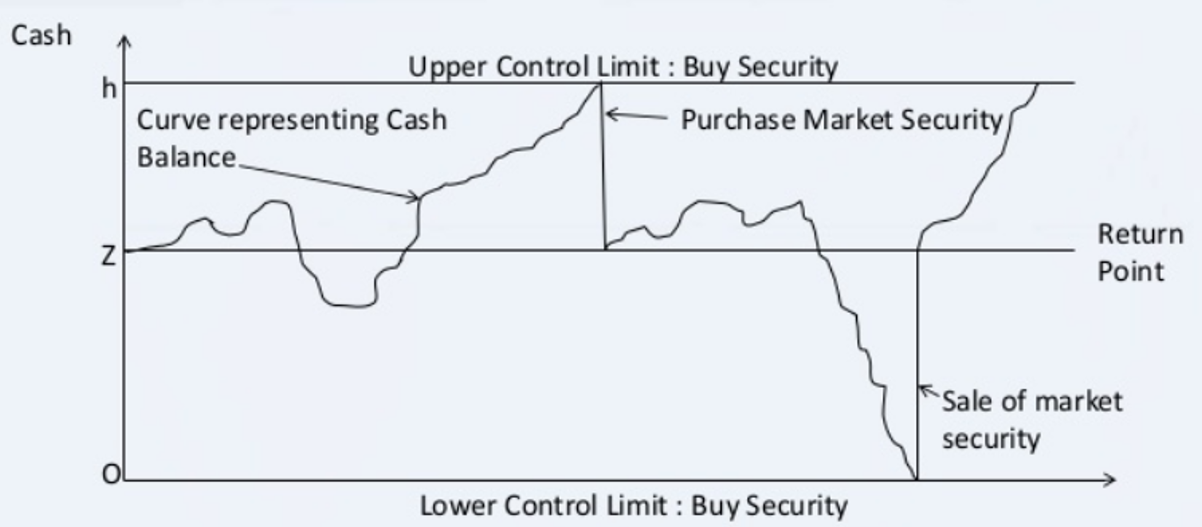
\includegraphics[scale=0.45 ,clip]
		{img/MillerOrr}
				
		\begin{align}
		Z^*&=\sqrt[3]{\frac{3 \cdot F \cdot \sigma^2}{4 \cdot (K/365)}}+L\\
		&=1 852 911\text{р.},\nonumber
		\end{align}
		где
		
		$Z^*$ - целевой ориентир баланса наличности;
		
		$F$ - Стоимость трансакции;

		$\sigma$ - стандартное отклонение дневного потока наличности в банке;

		$K$ - возможная стоимость денег для банка;

		$L$ - нижний предел уровня наличности.
		
	\end{solution}

\vfill\null\pagebreak
	\subpart[5] Определите верхний предел уровня наличности, при котором банк будет покупать высоколиквидные ценные бумаги, согласно модели Миллера-Орра.
	\begin{solution}[12em] 
		Верхний предел уровня наличности равен:
		\begin{align}
		H^*&=3 \cdot Z^* - 2 \cdot L\\
		&=3 558 733\text{р.}\nonumber
		\end{align}
	\end{solution}

	\subpart[5] Рассчитайте средний баланс наличности, который будет наблюдаться в кассах банка, при стратегии управления наличными по модели Миллера-Орра.
	\begin{solution}[12em]
		Средний баланс наличности равен:
		\begin{align}
		ABC&=\frac{4 \cdot Z^*-L}{3}\\
		&=2 137 214\text{р.}\nonumber
		\end{align}	
	\end{solution}
	
\end{subparts}
\addpoints

\subsection{Векселя}
\subsubsection{Дисконтный вексель}
\question[10] Вексель номиналом 500 000р. с датой погашения 27.02.20X(X+1) был учтен банком 19.11.20XX по простой учетной ставке 14,6\% годовых. Годы невисокосные. Какая сумма была выплачена банком?

\begin{solution}[12em]
	
	\raggedright
	Количество дней, оставшихся до погашения векселя: 100 дней.
	
	Тогда сумма к выплате составит:
	\begin{align*}
	500000 (1- 0,146 \cdot \frac{100}{365}) = 480 000\text{р.}
	\end{align*}
\end{solution}


\subsubsection{Форфейтинг}
\question[20] БД.К1.З4.В1,2. Российская фирма покупает у французской компании комплект оборудования стоимостью $P=1.1~M€$. Кредит предоставляется на срок $n=3$ года, выплаты в погашение основной суммы долга одинаковые и производятся один раз в год.
Продавец выписывает комплект переводных векселей в которых прописана сумма, равная стоимости отгружаемого товара и процентов за кредит, и направляет эти векселя покупателю для акцепта. Продавец использует простую ставку $i=5,25\%$ годовых для определения суммы процентов по векселю. 
Продавец, сражу же после получения портфеля акцептованных векселей, учитывает его в банке без права оборота на себя (форфейтинг), получая деньги в самом начале сделки. По форфейтной операции банк применяет простую учетную ставку в размере $d=5\%$ годовых.

\noaddpoints

\begin{subparts}
	\subpart[5] Определите номинальные суммы $V_t, t=1,n$ переводных векселей, выписанных экспортером и общую сумму денег, которую должен будет заплатить импортер. Результаты представьте в таблице.
	
	\begin{solution}[12em]
		
		Сумма векселя, погашаемого в момент времени $t$, равна:
		\begin{align}
		V_t=\frac{P}{n} \cdot \left(1+(n-t+1) \cdot i \right).
		\end{align}
		Общая сумма векселей равна:
		\begin{align}
		\sum_t V_t = P \cdot \left(1+ \frac{n+1}{2} \cdot i \right).
		\end{align}
		
	\end{solution}
	
	\subpart[5] Определите суммы $PV_t, t=1,n$, которые получит экспортер по каждому векселю, учтенному в банке и общий размер $A$ своей выручки. Результаты представьте в таблице. 
	
	\begin{solution}[12em]
		
		Экспортер получит в банке по каждому учтенному векселю следующую сумму:
		\begin{align}
		PV_t=V_t \cdot (1-t \cdot d)
		\end{align}
		и всего:
		\begin{align}
		A&=\sum_t V_t \cdot (1-t \cdot d)\nonumber\\
		&= \sum_{t=1}^{n}\frac{P}{n} \cdot \left( 1+ (n-t+1) \cdot i \right)	\cdot (1-t \cdot d)\nonumber\\
		&= P \cdot \left( 1+ \frac{n+1}{2} \cdot \left(i - d - i \cdot d \cdot \frac{n+2}{3} \right) \right)\\
		&=1 195 500~€.\nonumber
		\end{align}
		\begin{tabularx}{\linewidth}[b]{@{}>{\raggedright\arraybackslash}Xrrrr@{}}	
			\toprule
			Период & $\frac{P}{n}$ & \% & $V_t$ & $PV_t$ \\
			\midrule			
			\multicolumn{1}{l}{     1} & 400 000 & 63 000 & 463 000 & 439 850 \\
			\multicolumn{1}{l}{     2} & 400 000 & 42 000 & 442 000 & 397 800 \\
			\multicolumn{1}{l}{     3} & 400 000 & 21 000 & 421 000 & 357 850 \\
			\midrule			
			Итого & 1 200 000 & 126 000 & 1 326 000 & 1 195 500 \\
			\bottomrule
		\end{tabularx}%
	\end{solution}


	\subpart[10] Покроет ли выручка от учета векселей в банке стоимость отгруженной экспортером продукции? 
	
	Определите барьерную (минимальную) процентную ставку $i^*$, которую должен назначить экспортер, чтобы получить сумму больше, чем первоначальная цена продукции.
	
	\begin{solution}[12em]
		
		Экспортер получит сумму, меньшую первоначальной цены. 
		
		Продавец не будет иметь потери, если процентные ставки $i$ и $d$ находятся в следующем соотношении (вывод из предыдущего уравнения):
		\begin{align}
		i-d=i \cdot d \cdot \frac{n+2}{3}.
		\end{align}
		
		Поэтому барьерная процентная ставка равна:
		\begin{align}
		i^*&=\frac{d}{1-\frac{n+2}{3} \cdot d}\\
		&=5,45\%.\nonumber
		\end{align}
		
	\end{solution}


	
\end{subparts}
\addpoints

\vfill\null\pagebreak
\subsection{Управление банком}
\subsubsection{Рентабельность активов банка}
\question[10] Какова рентабельность активов банка, если рентабельность собственных средств - 45,5\%, причем собственные средства составляют 40\% от заемных? 

\begin{solution}[12em]
	\begin{align}
	R_E&=\frac{Pr}{E}\\
	R_A&=\frac{Pr}{E+D}\nonumber\\
	&=\frac{Pr/E}{(E+D)/E}\nonumber\\
	&=\frac{Pr/E}{1+\frac{1}{E/D}}\\
	&=\frac{0.455}{1+1/0.4}\nonumber\\
	&=0.13\nonumber
	\end{align}
	\raggedright
	где
	
	$Pr$ - прибыль банка;
	
	$E$ - величина собственных средств;
	
	$D$ - величина заемных средств;
	
	$R_E$ - рентабельность собственных средств;
	
	$R_A$ - рентабельность активов.
	
\end{solution}

\vfill\null\pagebreak
\subsubsection{Повышение доходности акций банка}
\question[20] БД.К1.З5.В1,2. Вы являетесь финансовым менеджером коммерческого банка ``ТФТ``. 
Показатели деятельности КБ ``ТФТ`` представлены в таблице.

		\begin{tabularx}{\linewidth}[b]{@{}>{\raggedright\arraybackslash}Xr@{}}	
		&млн. руб. \\
		\midrule
		Уставный фонд & 4500 \\
		Общие резервы & 500 \\
		Прибыль прошлых лет & 2000 \\
		Итого собственные средства & 7000 \\
		Срочные депозиты физических лиц & 5000 \\
		Депозиты до востребования юридических лиц & 1500 \\
		Срочные депозиты юридических лиц & 500 \\
		Итого привлеченные средства & 7000 \\
		\midrule
		Пассивы, всего & 14000 \\
		\midrule
		Активные операции &  \\
		\midrule
		Доли в общем объеме &  \\
		кредитование юридических лиц & 90\% \\
		вложения в ценные бумаги & 10\% \\
		\midrule
		Доходность &  \\
		кредитование юридических лиц & 13\% \\
		вложения в ценные бумаги & 25\% \\
		\midrule
		Ставки привлечения средств &  \\
		Срочные депозиты юридических лиц & 6\% \\
		Депозиты до востребования юридических лиц & 0,50\% \\
		Срочные депозиты физических лиц & 5\% \\
		\midrule
		Доли использования ресурсов банка в активных операциях &  \\
		собственные средства & 70\% \\
		депозиты до востребования & 30\% \\
		срочные депозиты & 100\% \\
		\midrule
		Норматив обязательных резервов по депозитам & 4,50\% \\
		Отчисления в фонд страхования вкладов физических лиц & 2\% \\
		Ставка налога на прибыль & 35\% \\
		Коэффициент выплат дивидендов (от прибыли после налогообложения) & 40\% \\
		Норматив отношения собственных и заемных средств, не менее & 15\% \\
		\bottomrule
	\end{tabularx}%
\noaddpoints

\begin{subparts}
	\subpart[5] Определите текущую доходность акций банка.
	
	\begin{solution}[12em]
		
	Текущий общий объем средств банка, направляемых на активные операции равен:
	
	СобСр * ДоляИспользованияСобСр + СрДепФизЛиц * (1 - НормРезДепоз) + СрДепЮрЛиц * (1- НормРезДепоз)  + ДоляИспольованияДепДовострЮрЛиц * ДепДовострЮрЛиц * (1- НормРезДепоз) = 10582.	
	
	
	ДоходностьАктивов = ДоляКредитовЮрЛицам * ДоходностьКредитовЮрЛицам + ДоляЦенныхБумаг * ДоходностьЦенныхБумаг = 14.2\%
	
	Доходы = Активы * ДоходностьАктивов = 1988
			
	Расходы = ПроцСрДепФизЛиц + ПроцСрДепЮрЛиц + ПроцДепДовострФизЛиц + ОтчСтрахВкл= 433
			
	ЧистаяПрибыль = (1- НалПриб) * (Доходы - Расходы) = 1011
			
	ДоходностьАкций = КоэфВыплДив * ЧистаяПриб / СобСр = 5.778\%
	
	\end{solution}
	
	\subpart[5] Предположим, что банку требуется повысить уровень доходности своих акций до 15\% годовых (Доходность акций рассчитывается как отношение фонда дивидендов к собственным средствам банка). Определите, будет ли достигнута эта цель, если банк направит всю чистую прибыль на выплату дивидендов?
	
	\begin{solution}[12em]
		
	Если банк направит всю чистую прибыль на выплату дивидендов, то доходность акций составит:
	
	ЧистаяПриб / СобСр = 14.444\%.
	
	Целевая доходность акций достигается.
	\end{solution}
	
	\subpart[10] Определите, какой объем срочных депозитов юридических лиц должен привлечь банк, чтобы достигнуть целевого уровня доходности своих акций. Будет ли банк в этом случае выполнять норматив по соотношению собственных и привлеченных средств?
		
	\begin{solution}[12em]
	
	Требуемый размер валовой прибыли для увеличения доходности акций до целевого уровня составит:
	
	СобСр * ТребуемаяДоходность / [КоэффициентВыплатДивидендов * (1 - СтавкаНалогаПрибыль)] = 4038,46
	
	Таким образом, валовая прибыль должна быть увеличена на 3172. 
		
	Процентная маржа, получаемая банком, за счет депозитов юридических лиц равна:
	
	ПроцМаржаСрочДепозЮрЛиц = ДоходностьАктивов * (1 - НормаОбязательныхРезервов) -
	СтСрочДепозЮрЛиц = 7.56\%
	
	ПриростСрочДепозЮрЛиц =  ПриростПрибыли / ПроцентнаяМаржа = 40039
			
	Новое соотношение собственных и привлеченных средств банка при этом составит:
	
	СобСр / (ПривлечСр + ПриростСрочДепозЮрЛиц) = 14.88\%
	
	Таким образом, требование регулятора о соотношении собственных и заемных средств банка не выполняются. 		
	\end{solution}
\end{subparts}
\addpoints

\subsubsection{Увеличение объема активных операций банка}
\question[20] Вы являетесь финансовым менеджером коммерческого банка "Барс". 
Показатели деятельности КБ "Барс" представлены в таблице.

\begin{tabularx}{\linewidth}[b]{@{}>{\raggedright\arraybackslash}Xr@{}}	
	&млн. руб. \\
	\midrule
	Уставный фонд & 4000 \\
	Общие резервы & 100 \\
	Прибыль прошлых лет & 50 \\
	Итого собственные средства & 4 150 \\
	Срочные депозиты физических лиц & 10000 \\
	Депозиты до востребования юридических лиц & 6500 \\
	Срочные депозиты юридических лиц & 10500 \\
	Итого привлеченные средства & 27 000 \\
	\midrule
	Пассивы, всего & 31 150 \\
	\midrule
	Активные операции &  \\
	\midrule
	Доли в общем объеме &  \\
	кредитование юридических лиц & 80\% \\
	вложения в ценные бумаги & 20\% \\
	\midrule
	Доходность &  \\
	кредитование юридических лиц & 12\% \\
	вложения в ценные бумаги & 20\% \\
	\midrule
	Ставки привлечения средств &  \\
	Срочные депозиты юридических лиц & 3\% \\
	Депозиты до востребования юридических лиц & 0,50\% \\
	Срочные депозиты физических лиц & 5\% \\
	\midrule
	Доли использования ресурсов банка в активных операциях &  \\
	собственные средства & 70\% \\
	депозиты до востребования & 73\% \\
	срочные депозиты & 100\% \\
	\midrule
	Норматив обязательных резервов по депозитам & 2,50\% \\
	Отчисления в фонд страхования вкладов физических лиц & 2\% \\
	Ставка налога на прибыль & 35\% \\
	Норматив отношения собственных и заемных средств, не менее & 15\% \\	
	\bottomrule
\end{tabularx}%
\noaddpoints

\vfill\null\pagebreak
\begin{subparts}
	\subpart[5] Определите текущую доходность акций банка (Доходность акций рассчитывается как отношение фонда дивидендов к собственным средствам банка). 

\begin{solution}[12em]
	
	Текущий общий объем средств банка, направляемых на активные операции равен:
	
	СобСр * ДоляИспользованияСобСр + СрДепФизЛиц * (1 - НормРезДепоз) + СрДепЮрЛиц * (1- НормРезДепоз)  + ДоляИспольованияДепДовострЮрЛиц * ДепДовострЮрЛиц * (1- НормРезДепоз) = 27519
			
	ДоходностьАктивов = ДоляКредитовЮрЛицам * ДоходностьКредитовЮрЛицам + ДоляЦенныхБумаг * ДоходностьЦенныхБумаг = 13.6\%
	
	Доходы = Активы * ДоходностьАктивов = 4236
	
	Расходы = ПроцСрДепФизЛиц + ПроцСрДепЮрЛиц + ПроцДепДовострФизЛиц + ОтчСтрахВкл = 1005
			
	ЧистаяПрибыль = (1 - СтНалПриб) * (Доходы - Расходы) = 2100
			
	ДоходностьАкций = ЧистаяПриб / СобСр = 50.6\%
	
\end{solution}
	
	\subpart[5] Предположим, что банку требуется увеличить объем активных операций на 7\%. Определите, сможет ли банк достигнуть эту цель, за счет изменения порядка распределения прибыли (уменьшения ее доли, направляемой в фонд дивидендов, и увеличения за счет этого объемов кредитования)? Является ли этот вариант приемлемым для банка с точки зрения собственников банка, получающих дивиденды на свои вложения?
	
	\begin{solution}[12em]
		
		УвелАктОпераций = Активы * ПроцРостаАктивныхОпераций = 2180
		
		Текущей прибыли достаточно. 
		
		Доходность акций банка в этом случае составит:
		
		(ЧистаяПриб - УвелАктОпераций) / СобсСр = 1.2\%.
		
		Несмотря на значительное снижение доходности акций, данный вариант увеличения объема активных операций является для банка единственно возможным из рассмотренных (см. расчеты далее).		
	\end{solution}
	
	\subpart[10] Какой объем вкладов срочных депозитов физических лиц должен привлечь банк, чтобы достигнуть целевого объема активных операций. Будет ли банк в этом случае выполнять норматив по соотношению собственных и привлеченных средств?
		
	\begin{solution}[12em]
	
	ДопДепозитыФизЛиц = УвелАктОпераций /(1 - НормРезДепоз) = 2236
		
	ПроцМаржаСрочДепозФизЛиц
	 = ДоходностьАктивов * (1 - НормаОбязательныхРезервов - ОтчисленияФондСтрахованияВкладовФЛ) - СтоимостьДепозитовФЛ = 8.49\%. 
	
	Соответственно, валовая прибыль банка увеличится за счет дополнительных депозитов физических лиц на:
	
	ПриростЧистойПрибыли = ДопДепозитыФизЛиц * ПроцМаржаСрочДепозФизЛиц * (1- НалПриб) = 123
			
	Новая доходность акций: 53.59\%
	
	СобСр / ЗаемСр = СобСр / (ПривСр + ДопДепозитыФизЛиц) = 14.19\%.
	
	Требования регулятора не выполняются. 
	
	\end{solution}
\end{subparts}
\addpoints

\subsubsection{Выпуск ипотечных облигаций банком}
\question[20] В январе 20XX г. коммерческому банку "Коралл" с уставным капиталом 150млн. руб. предоставлен льготный государственный кредит для обеспечения долгосрочного кредитования населения на покупку жилья. Кредит выдан в размере 100млн. руб. под 4,5\% годовых на 30 лет. В течение января — марта 20XX г. за счет полученного кредита банком были выданы следующие ипотечные ссуды физическим лицам.

	\begin{tabularx}{\linewidth}[b]{@{}>{\raggedright\arraybackslash}Xrr@{}}	\toprule
		Категория кредита &млн. руб. & Cтавка, \% \\
		\midrule
		Кредиты на срок до 10 лет & 30    & 6,00\% \\
		Кредиты на срок от 10 до 15 лет & 25    & 7,00\% \\
		Кредиты на срок от 15 до 20 лет & 19    &  8,00\% \\
		Кредиты на срок свыше 20 лет & 8     &  10,00\% \\
		\midrule
		Итого & 82    & ??? \\
		\bottomrule
	\end{tabularx}%

Кроме того, в течение апреля 20XX года в банк обратились еще 100 клиентов с целью получения долгосрочных кредитов на строительство жилья. Из всех поступивших кредитных заявок отбор прошли заявки 30 клиентов на общую сумму 60млн. руб. Планируемая средняя ставка по данным кредитам составляет 15\% годовых. 

Ставка налога на прибыль	35\%.
Коэффициент выплат дивидендов из прибыли после налогообложения	75\%.

\noaddpoints

\begin{subparts}
	\subpart[10]  Определите доходность акций банка при удовлетворении поступивших заявок на ипотечный кредит в сумме 18 млн. рублей.
	
	\begin{solution}[12em]
		
		Процентные доходы банка по выданным ипотечным кредитам составят:
		
		ПроцДоходы = СУММПРОИЗВ = 5,87млн. руб.
		
		Процентные доходы банка по дополнительным ипотечным кредитам составят:
		
		ДопДох = (ЛьготКредит - Выданные кредиты) * ПланСтКред = 2,7млн. руб.
		
		Процентные расходы банка равны суммам процентов, выплачиваемым по льготному государственному кредиту:
		
		ПроцРасх = ЛьготныйКредит * СтПроцЛьготныйКредит = 4,5млн. руб. 
		
		ЧистПриб = (ПроцДоходы + ДопДох - ПроцРасх) * (1 - СтНалПриб) = 2,65млн. руб.
		
		ДоходностьАкций = ЧистаяПрибыль * КоэфВыплатДивидендов / СобСр = 1,32\%
		
	\end{solution}
	
	\subpart[10] Предположим, что остальные одобренные заявки банк может выполнить за счет выпуска ипотечных облигаций и дополнительного привлечения депозитов физических лиц. 
	
	Условия выпуска облигаций следующие:
	\begin{easylist}[itemize]	
	& облигации могут быть эмитированы на сумму не более 80\% стоимости выданных ипотечных кредитов и не более 25\% уставного фонда;
	
	& облигации процентные, с выплатой 5\% годовых;
	
	& анализ спроса на рынке капиталов показал, что банк сможет привлечь 34.4~млн. рублей за счет выпуска ипотечных облигаций в течение года.
	\end{easylist}
	Долгосрочные депозиты физических лиц банк может привлечь под 9\% годовых.
	
	На основании представленных данных определите удовлетворения дополнительных заявок на ипотечный кредит, исходя из критерия доходности акций.
	Доходность акций рассчитывается как отношение фонда дивидендов к уставному капиталу банка. 
	
	Определите, какой объем ипотечных облигаций и какой объем депозитов должен привлечь банк?
	
	\begin{solution}[12em]
		
		Требуемая дополнительная величина ресурсов для банка составит:
		
		ПриростПривлСредств = ЗаявкиДополнительныеКредиты – (ЛьготныйГосударственныйКредит – ВыданныеИпотечныеКредиты) = 42млн. руб.
		
		За счет выпуска ипотечных облигаций можно профинансировать 34,4~млн.р. этой суммы.
		
		ДопустимыйОбъемВыпуска = МИН(УставныйКапитал * Доля облигаций от уставного капитала; ПриростДепФизЛиц * Доля облигаций от требуемого объема средств) = 33,6млн. руб.
		
		Остальные привлеченные средства должны составить долгосрочные депозиты.
		
		ПриростДепФизЛиц = ПриростПривлСредств - ДопустимыйОбъемВыпуска = 8,40	
		
	\end{solution}

	\subpart[10] Определите доходность акций банка, в случае полного удовлетворения заявок на ипотечный кредит. Является ли этот вариант более выгодным, по сравнению с отказом в кредите тем заемщикам, для удовлетворения заявок которых льготного государственного кредита оказалось недостаточно?

	\begin{solution}[12em]
		
		Процентные доходы банка по ипотечным кредитам составят:
		
		ПроцДоходыВсего = ПроцДоходы + ЗаявкиДополнительныеКредиты * ПланСтКред	 = 14,87млн. руб.
		
		ПроцРасхВсего = ПроцЛьготКред + ПроцОблиг + ПроцДепФизЛиц = 6,936
		
		ЧистПриб = (ПроцДоходыВсего - ПроцРасхВсего) * (1 - СтНалПриб) = 5,157
		
		ДоходностьАкций = ЧистПриб * КоэфВыплДив / СобСр = 2,58\%.
		
		Таким образом, выпуск ипотечных облигаций и удовлетворение поступивших ипотечных заявок на кредит в полном объеме приведет к увеличению доходности акций банка, следовательно, данный вариант предпочтительнее.
		
	\end{solution}
	
\end{subparts}
\addpoints

\subsubsection{Карточный зарплатный проект банка}
\question[20] Банк рассматривает целесообразность внедрения на предприятии карточного зарплатного проекта.

Общий фонд оплаты труда составляет 4 250 000р. (количество работников – 350 чел.). Выплаты производятся регулярно, общее финансовое состояние предприятия среднее. Предприятие предполагает выпуск 5 карт типа Gold, 10 карт типа Standart и остальные - Cirrus/Maestro. Также предприятие планирует установку одного банкомата на главной проходной. Получение денежных средств в устанавливаемых банкоматах предполагается бесплатным.

За перечисление средств на счета банк берет комиссию 0,15\%.
Стоимость поддержания каждой карты в базе данных процессингового центра составляет 5р. в месяц. Стоимость процессинга операций выдачи наличных - 0,1\% с оборота (при этом исходя из анализа рынка считается, что 75\% поступлений на картсчета снимаются наличными).

Стоимость банкоматов рассчитывается исходя из цены 450 000р. за устройство. Инкассация банкоматов производится 2 раза в месяц (1300р. за выезд).
Для оценки общего размера привлеченных средств в расчет следует принять, что работники предприятия будут оставлять на карточных счетах в среднем не более 25\% от фонда оплаты труда, банк имеет возможность инвестирования этих средств по ставке 23\% годовых с учетом себестоимости операций в 1\%.

Ставка рефинансирования составляет 13\%. Стоимость карт указана в таблице.

	\begin{tabularx}{\linewidth}[b]{@{}>{\raggedright\arraybackslash}Xrrr@{}}	\toprule
		Тип карты & Кол-во, шт. & Себест. ед.& Цена ед., р. \\
		\midrule
		Gold  & 5     & 175   & 1250 \\
		Standart & 10    & 125   & 250 \\
		Cirrus/Maestro & 335   & 75    & 125 \\
		\bottomrule
	\end{tabularx}%

\noaddpoints

\begin{subparts}
		\subpart[5] Определите единовременный доход, который получит банк в результате эмиссии банковских карт. 
	
	\begin{solution}[12em]
		
		Банк получит следующий доход в момент продажи карт клиентам (рублей):
		
		\begin{tabularx}{\linewidth}[b]{@{}>{\raggedright\arraybackslash}Xrrrrr@{}}	\toprule
			Тип карты & Кол-во, шт. & Себест. ед. & Себест. общ. & Цена ед., р. & Выручка \\
			\midrule
			Gold  & 5     & 175   & 875   & 1250  & 6250 \\
			Standart & 10    & 125   & 1250  & 250   & 2500 \\
			Cirrus/Maestro & 335   & 75    & 21125 & 125   & 41875 \\
			\midrule
			Итого & 350   &       & 27250 &       & 50625 \\
			\bottomrule
		\end{tabularx}%
						
	\end{solution}
	
	\subpart[10] Определите ожидаемые доходы и расходы, а также денежный поток проекта на временном интервале 3 года. 
	
	\begin{solution}[12em]
		
		Денежный поток от инвестиций определен в таблице:
				
			\begin{tabularx}{\linewidth}[b]{@{}>{\raggedright\arraybackslash}Xrrrr@{}}	\toprule
				Доходы и расходы & 0 год & 1 год & 2 год & 3 год \\
				\midrule
				Доход от выдачи карт &       & 50625 &       &  \\
				Операционный доход от перечислений на картсчета &       & 76500 & 76500 & 76500 \\
				Доход от размещения привлеченных средств &       & 244375 & 244375 & 244375 \\
				\midrule
				Итого доходов &       & 371500 & 320875 & 320875 \\
				\midrule
				Себестоимость пластика & 27250 &       &       &  \\
				Затраты на банкоматы & 450000 & 31200 & 31200 & 31200 \\
				Затраты на процессинг &       & 59250 & 59250 & 59250 \\
				Начисление процентов на остатки на картсчетах &       & 10625 & 10625 & 10625 \\
				\midrule
				Итого расходов &       & 101075 & 101075 & 101075 \\
				\midrule
				Денежный поток & 477250 & 270425 & 219800 & 219800 \\
				\bottomrule
			\end{tabularx}%
				
	\end{solution}
	
	\subpart[5] Рассчитайте чистую приведенную стоимость инвестиций банка в зарплатный проект и сделайте выводы относительно его окупаемости. Если проект окажется окупаемым, предложите способы повышения его окупаемости. Если проект окажется неокупаемым,  предложите мероприятия по достижению окупаемости.
	
	\begin{solution}[12em]
	
		Величину получаемого денежного потока следует дисконтировать к моменту начала проекта, использую ставку рефинансирования Банка России, 13\%.
		
		\begin{align*}
		\text{Дисконтированный поток} &= \frac{270425}{1,13}  + \frac{219800}{1,13^2} + \frac{219800}{1,13^3} \\
		&= 563 782p
		\end{align*}
		
		
		Полученная сумма оказалась больше вложенных инвестиций, следовательно, проект окупается. Для улучшения его привлекательности можно повышать стоимость обслуживания, учитывая, что чрезмерная дороговизна может привести к отказу от проекта со стороны предприятия.
			
	\end{solution}
	
\end{subparts}
\addpoints

\subsubsection{Баланс банка}
\question[10] На основании нижеприведенных данных составьте баланс коммерческого банка.

	\begin{tabularx}{\linewidth}[b]{@{}>{\raggedright\arraybackslash}cXr@{}}
		№     & &млн. руб.\\
		\midrule
		1     & Корреспондентские счета других коммерческих банков & 6,7 \\
		2     & Дебиторы банка & 55,4 \\
		3     & Корреспондентские счета в других коммерческих банках & 65,2 \\
		4     & Кредиты, полученные от других коммерческих банков & 54,7 \\
		5     & Уставный фонд & 37,2 \\
		6     & Прочие активы & 130,1 \\
		7     & Вложения в государственные облигации & 10,4 \\
		8     & Ссудные счета предприятий & 162,7 \\
		9     & Резервные счета в Банке России & 15,3 \\
		10    & Прочие пассивы & 144,9 \\
		11    & Прочие фонды & 39,1 \\
		12    & Доходы & 167,5 \\
		13    & Текущие счета клиентов & 148,2 \\
		14    & Здания и сооружения & 159,2 \\
		\bottomrule
	\end{tabularx}%

\begin{solution}[12em]
	
	\begin{tabularx}{\linewidth}[b]{@{}>{\raggedright\arraybackslash}XrXr@{}}
			Актив & млн. руб. & Пассив & млн. руб. \\
			\midrule
			Здания и сооружения & 159,2 & Текущие счета клиентов & 148,2 \\
			Ссудные счета предприятий & 162,7 & Доходы & 167,5 \\
			Резервные счета в Банке России & 15,3  & Прочие пассивы & 144,9 \\
			Прочие активы & 130,1 & Прочие фонды & 39,1 \\
			Вложения      в государственные облигации & 10,4  & Кредиты, полученные от других коммерческих банков & 54,7 \\
			Корреспондентские счета в других коммерческих банках & 65,2  & Уставный фонд & 37,2 \\
			Дебиторы банка & 55,4  & Корреспондентские счета других коммерческих банков & 6,7 \\
			\midrule
			Итого & 598,3 & Итого & 598,3 \\
			\bottomrule
		\end{tabularx}%
	
\end{solution}

\subsubsection{Отчет о прибылях и убытках банка}
\question[10] На основании данных о величине доходов и расходов (таблица 1) определить:

1.	Финансовый результат деятельности банка.

2.	Размер банковской маржи.

	\begin{tabularx}{\linewidth}[b]{@{}>{\raggedright\arraybackslash}cXr@{}}
		\toprule
		№     & Показатели &млн. руб. \\
		\midrule
		1     & Проценты, полученные за предоставленные кредиты & 15,2 \\
		2     & Доходы, полученные от операций с ценными бумагами & 8,1 \\
		3     & Доходы, полученные от операций с иностранной валютой & 4,8 \\
		4     & Другие доходы & 4,9 \\
		5     & Проценты, уплаченные за привлеченные кредиты & 1,2 \\
		6     & Проценты, уплаченные юридическим лицам по привлеченным средствам & 1,9 \\
		7     & Проценты, уплаченные физическим лицам по депозитам & 7,9 \\
		8     & Расходы по операциям с ценными бумагами & 4,8 \\
		9     & Расходы по операциям с иностранной валютой & 1,2 \\
		10    & Расходы на содержание аппарата управления & зд \\
		11    & Штрафы, пени, неустойки уплаченные & 0,1 \\
		12    & Другие расходы & 10,3 \\
		\bottomrule
	\end{tabularx}%


\begin{solution}[12em]

\raggedright
1)	Доходы банка составляют: 15,2 + 8,1 + 4,8 + 4,9 = 33,0млн. руб. 

Расходы банка составляют: 1,2 + 1,9 + 7,9 + 4,8 + 1,2 + 3,1 + 0,1 + 10,3 =
30,5млн. руб.

Финансовый результат: 33,0 - 30,5 = 2,5млн. руб.

2)	Банковская маржа составляет: 15,2 - (1,2 + 1,9 + 7,9) = 4,2млн. руб. 
\end{solution}

\subsubsection{Норматив долгосрочной ликвидности}
\question[10] Собственные средства (капитал) банка на отчетную дату составили 680 000p Обязательства банка со сроком, оставшимся до погашения, свыше одного года составляют 560 000p 
\noaddpoints

\begin{subparts}
	\subpart[5] Определите	максимальную сумму долгосрочных кредитов, которую может выдать банк при соблюдении норматива долгосрочной ликвидности.
	
	\begin{solution}[12em]
		Н4 - норматив долгосрочной ликвидности - рассчитывается по формуле:
		
		\begin{align}
		\text{Н4} = \frac{\text{Крд}}{\text{К} + \text{ОД}} \leq 120\%,
		\end{align}
		
		где Крд – кредитные требования с оставшимся сроком до даты погашения свыше 1 года (долгосрочные кредиты);
		
		К – собственные средства (капитал) банка;
		
		ОД – обязательства банка со сроком, оставшимся до погашения, свыше одного года (долгосрочные обязательства).
		
		Отсюда, максимальная сумма долгосрочных кредитов:
		
		Крд = мах Н4 * (К + ОД)
		
		Крд = 120\% / 100\% * (680 000 + 560 000) = 1 488 000р.
		
	\end{solution}
	
	\subpart[5] Определите	максимальную сумму, на которую банк может увеличить портфель долгосрочных кредитов, если норматив долгосрочной ликвидности на отчетную дату составляет 93\%.
		
	\begin{solution}[12em]
		Если Н4 составляет 93\%, то сумма долгосрочных кредитов на отчетную дату равна:
		
		Крд = 93\% / 100\% * (680 000 + 560 000) = 1 153 000p
		
		Максимальная сумма долгосрочных кредитов банка при заданной величине капитала и долгосрочных обязательств рассчитана в первом действии и составляет 1 488 000p
		
		Соответственно, банк может увеличить сумму долгосрочных кредитов только до этой максимальной величины, то есть на величину, равную:
		
		1 488 000 – 1 153 000 = 335 000p
		
	\end{solution}
	
\end{subparts}
\addpoints



\cleardoublepage
\section{Финансовые рынки}
\subsection{Облигации}
\subsubsection{Рыночная цена облигации}
\question[10] Номинал облигации 1000р., купон 10\%, выплачивается один раз в гол. До погашения облигации 3 года. Определить цену облигации, если её доходность до погашения должна составить 8\%.

\begin{solution}[12em]
	\begin{align}
	P=\frac{C}{1+r} + \frac{C}{(1+r)^2} + + \frac{C+N}{(1+r)^n},
	\end{align}
	\raggedright
	где
	
	$P$ - цена облигации;
	
	$C$ - купон в рублях;
	
	$N$ - номинал;
	
	$n$ - число лет до погашения облигации;
	
	$r$ - доходность до погашения облигации.
	
	Ответ: 1051.54p
\end{solution}


\question[10] Номинал облигации 1000р. купон 10\%. выплачивается два раза в год. До погашения облигации 2 года. Определить цену облигации, если ее доходность до погашения должна составить 8\%.

\begin{solution}[12em]
	\raggedright
	Когда купон выплачивается m раз в год, то:
	\begin{align}
	P=\frac{C/m}{1+r/m} + \frac{C/m}{(1+r/m)^2} + + \frac{C/m+N}{(1+r/m)^{mn}}
	\end{align}
	Ответ: 1036.3p
	
	Примечание.
	
	Данную задачу можно решить, используя формулу для $m=1$, только в этом случае периоды времени выплаты купонов следует учитывать не в купонных периодах, а как и раньше, в годах. Первый купон выплачивается через полгода, поэтому для него время выплаты равно 0.5 года, второй купон выплачивается через год, для него время выплаты равно 1 год и т.д. Ставка дисконтирования учитывается в этом случае как эффективный процент на основе заданной доходности до погашения, т.е. она равна:
	\begin{align*}
	(1+0.08/2)^2-1=0.0816.
	\end{align*}
	
\end{solution}



\question[10] Номинал облигации 1000р., купон 10\%. выплачивается один раз в год. До погашения облигации 2 года 250 дней. Определить цену облигации, если ее доходность до погашения должна составить 8\%. База 365 дней.

\begin{solution}[12em]
	\begin{align}
	\frac{100}{1.08^{\frac{250}{365}}} + \frac{100}{1.08^{1\frac{250}{365}}} +\frac{100}{1.08^{2\frac{250}{365}}}=1077.35\text{р.}
	\end{align}
\end{solution}


\question[10] Номинал облигации 1000р., купон 10\%. Выплачивается один раз в год. До погашения облигации 15 лет. Определить цену облигации, если ее доходность до погашения должна составить 11.5\%.

\begin{solution}[12em]
	\begin{align}
	P&=\frac{C}{r} \cdot \left[1- \frac{1}{(1+r)^n} \right] + \frac{N}{(1+r)^n}\\
	&=895.05\text{р.}\nonumber
	\end{align}
\end{solution}


\question[10] Номинал облигации 1000р., купон 10\%, выплачивается два раза в год. До погашения облигации 6 лет. Определить цену облигации, если ее доходность до погашения должна составить 8,4\% годовых.

\begin{solution}[12em]
	\begin{align}
	P&=\frac{C}{r} \cdot \left[1- \frac{1}{(1+r/m)^{mn}} \right] + \frac{N}{(1+r/m)^{mn}}\\
	&=1074.22\text{р.}\nonumber
	\end{align}
\end{solution}


\question[10] Номинал облигации 1000р., купон 7\%. выплачивается один раз в год. До погашения облигации 11 дет и 45 дней. Определить цену облигации, если ее доходность до погашения должна составить 8\%. База 365 дней.

\begin{solution}[12em]
	\begin{align}
	P&=\frac{1}{(1+r)^{\frac{t}{\text{база}}}} \left[\frac{C}{r} \cdot \left[1- \frac{1}{(1+r)^n} \right] + \frac{N}{(1+r)^n} \right]\\
	&=989,18\text{р.}\nonumber
	\end{align}
\end{solution}


\question[10] Номинал бескупонной облигации равен 1000р. бумага погашается через 5 дет. Определить цену облигации, если ее доходность до погашения должна составить 12\% годовых.

\begin{solution}[12em]
	\begin{align}
	??
	\end{align}
\end{solution}


\question[10] Номинал бескупонной облигации ранен 1000р. бумага погашается через 5 лет н 20 дней. Определить цену облигации, если се доходность до погашения должна составить 12\% годовых. База 365 дней.

\begin{solution}[12em]
	\begin{align}
	P&=\frac{N}{(1+r)^n}\\
	&=\frac{100}{1.12^{5\frac{20}{365}}}\nonumber\\
	&=567.43\text{р.}\nonumber
	\end{align}
\end{solution}


\question[10] Номинал бескупонной облигации равен 1000р., бумага погашается через 7 дет. Определить цену облигации, если ее доходность до погашения должна составить 8\% годовых. По купонным облигациям купоны выплачиваются два раза в год.

\begin{solution}[12em]
	\begin{align}
	P&=\frac{N}{(1+r/m)^{mn}}\\
	&=577.48\text{р.}\nonumber
	\end{align}
\end{solution}

\question[10] Номинал бескупонной облигации равен 1000р., бумага погашается через 30 дней. Определить цену облигации, если ее доходность до погашения должна составить 4\% годовых. База 365 дней.

\begin{solution}[12em]
	\begin{align}
	P&=\frac{N}{1+ \frac{r \cdot t }{\text{база}}}\\
	&=996.72\text{р.}\nonumber
	\end{align}
\end{solution}

\subsubsection{Доходность облигации}

\question[10] Номинал облигации 1000р., купон 10\%. Облигация стоит 953p Определить текущую доходность облигации.

\begin{solution}[12em]
	\begin{align}
	r_T&=\frac{C}{P}\\
	&=10.49\%\nonumber
	\end{align}
\end{solution}


\question[10] Номинал бескупонной облигации равен 1000р., бумага погашается через 3 года. Облигация стоит 850p Определить доходность до погашения облигации.

\begin{solution}[12em]
	\begin{align}
	r&=\sqrt[n]{\frac{N}{P}}-1\\
	&=5.57\%.
	\end{align}
\end{solution}


\question[10] Номинал бескупонной облигации равен 1000p бумага погашается через 4 года и 120 дней. Облигация сюит 640p Определить доходность до погашения облигации. База 365 дней.

\begin{solution}[12em]
	\begin{align*}
	r=\sqrt[4\frac{120}{365}]{\frac{1000}{640}} - 1 = 10.86\%.
	\end{align*}
\end{solution}



\question[10] Номинал бескупонной облигации 1000p Облигация погашается через три гола. Инвестор купил облигацию по 850p и продал через один гол 64 дня по 910p Определить доходность операции инвестора в расчете на год 1) на основе простого процента; 2) эффективного процента. База 365 дней.

\begin{solution}[12em]
	\begin{align*}
	&1) \left(\frac{873}{850} - 1 \right) \cdot \frac{365}{120}=8.23\%;\\
	&2) \left(\frac{873}{850} \right)^{\frac{365}{120}}=8.46\%.
	\end{align*}
\end{solution}

\subsubsection{Бескупонные облигации}
\question[10] Предприятие продает банку бескупонную облигацию номинальной стоимостью 500000p Оставшийся срок обращения облигации 25~дней. Учетная ставка 6\% годовых.

\noaddpoints
\begin{subparts}
	\subpart[8] Определите сумму, которую банк заплатит клиенту.
	\begin{solution}[8em]
		\begin{align}
		P&=N \cdot \left(1 - r \cdot \frac{n}{365} \right)\\
		&= 497945.21\text{р.}\nonumber
		\end{align}
		где
		
		$P$ - рыночная цена облигации, $N$ - номинал облигации, $r$ - учетная ставка, $n$ - оставшийся срок до погашения облигации в днях. 
	\end{solution}
	
	\subpart[2] Определите рыночный курс облигации (отношение рыночной цены к номиналу).
	\begin{solution}[4em]
		\begin{align}
		K&=\frac{P}{N}\\
		&=99,59\%\nonumber
		\end{align}
	\end{solution}
\end{subparts}
\addpoints


\question[10] Номинал краткосрочной бескупонной облигации 1000р., цена 950p Облигация погашается через 200 дней. Определить доходность до погашения облигация. База 365 дней.

\begin{solution}[12em]
	\begin{align}
	r&=\left(\frac{N}{P} -1 \right) \cdot \frac{\text{база}}{t}\\
	&=9.61\%.\nonumber
	\end{align}
\end{solution}

\question[10] Номинал облигации 1000р., цена 994p Облигация Погашается через 32 дня. Определить доходность до погашения облигации. База 365 дней. Определите эффективную доходность облигации.

\begin{solution}[12em]
	
	\raggedright
	Ответ: 6,89\%.
\end{solution}


\question[10] Номинал облигации 1000р., купон 6\%. выплачивается одни раз в год. Облигация погашается через три года. Инвестор купил облигацию по 850р. и продал через 57 дней по 859p За период владения облигацией купон по бумаге не выплачивался. Определить доходность операции инвестора: 1)~в расчете на 57 дней: 2)~в расчете на год на основе простого процента; 3)~эффективный процент по операции. База 365 дней.

\begin{solution}[12em]
	\begin{align*}
	&1)\space \frac{859}{850} - 1 = 1.06\%;\\
	&2)\space \left(\frac{859}{850} - 1 \right)^{\frac{365}{57}}=6.78\%;\\
	&3)\space \left(1+ 0.0106 \right)^{\frac{365}{57}}=6.99\%.
	\end{align*}
\end{solution}

\subsubsection{Бессрочная облигация}
\question[10] ДКБ.К1.З3.В1,2.Предположим, что бессрочная облигация дает ежегодный доход 3600p
\noaddpoints
\begin{subparts}
	\subpart[5] Определите ожидаемую рыночную цену такой облигации, если доходность других активов с тем же уровнем риска составляет 6\%.
	
	\begin{solution}[12em]
		\begin{align}
		P_1&=\frac{C}{r_1}\\
		&=60000\text{р.},\nonumber
		\end{align}	
		где
		
		$P_1$ - рыночная цена облигации;
		
		$C$ - купонный доход,р.;
		
		$r_1$ - процентная ставка, годовых.
	\end{solution}
	
	\subpart[5] Если доходность других активов вырастет до 10\%, то повысится или снизится рыночная цена этой облигации и до какого уровня.
	
	\begin{solution}[12em]
		\begin{align*}
		P_2=\frac{C}{r_2}=36000\text{р.}
		\end{align*}	
		
	\end{solution}
\end{subparts}
\addpoints

\subsubsection{Доходность долгосрочных облигаций (определение по таблицам)}
\question[10] Обратитесь к данным табл. и рассчитайте доходность при погашении облигации номиналом 1000~\$, со сроком погашения 6 лет, номинальной доходностью 6\% и текущей ценой 906,10~\$.

Доходность при погашении облигаций с номинальной доходностью 6\%.

\centering
\begin{tabularx}{.52\textwidth}[b]{@{}>{\raggedright\arraybackslash}crrrrr@{}}
	\toprule
	\% г-вых & \multicolumn{5}{c}{Годы до погашения} \\\cmidrule{2-6}
	& 6     & 6½    & 7     & 7½    & 8 \\
	\midrule		 
	7     & 95,17 & 94,85 & 94,54 & 94,24 & 93,95 \\
	7,2   & 94,24 & 93,86 & 93,49 & 93,14 & 92,8 \\
	7,4   & 93,31 & 92,88 & 92,46 & 92,05 & 91,66 \\
	7,6   & 92,4  & 91,91 & 91,44 & 90,98 & 90,54 \\
	7,8   & 91,5  & 90,96 & 90,43 & 89,92 & 89,44 \\
	8     & 90,61 & 90,01 & 89,44 & 88,88 & 88,35 \\
	\bottomrule
\end{tabularx}%

\begin{solution}[12em]
	
	\raggedright	
	Ответ: доходность при погашении 8\%.
\end{solution}

\subsubsection{Метод линейной интерполяции для определения доходности долгосрочных облигаций}
\raggedright	
\question[20] ДКБ.К1.З4.В1,2. МОФР.К1.З1.В1,2. Номинал облигации 1000р., купон 7\%, выплачивается один раз в год. До погашения облигации 5 лет. Облигация стоит 890p 
\noaddpoints
\begin{subparts}
	\subpart[10] Определите ориентировочно доходность до погашения облигации.
	\begin{solution}[12em]
		\begin{align}
		r^*&=\frac{(N-P)/m \cdot n + C/m }{(N+P)/2}\\
		r^*&=9,74\%\nonumber
		\end{align}
		где
		
		$r^*$ - ориентировочная доходность облигации;
		
		$N$ - номинал облигации;
		
		$P$ - рыночная цена облигации;
		
		$C$ - сумма купона;
		
		$n, m$ - срок облигации и количество выплат процентов в году, соответственно.
	\end{solution}
	
	\subpart[10] Определите доходность до погашения облигации методом линейной интерполяции.
	
	\begin{solution}[12em]
		\begin{align}
		r_1&=10\%\nonumber\\
		r_2&=9\%\nonumber\\
		P_1&=\frac{C}{r_1} \cdot \left(1 - \frac{1}{(1+r_1)^n} \right) + \frac{N}{(1+r_1)^n}\\
		&=886,277\text{р.}\nonumber\\
		P_2&=\frac{C}{r_2} \cdot \left(1 - \frac{1}{(1+r_2)^n} \right) + \frac{N}{(1+r_1)^n}\\
		&=922,21\text{р.}\nonumber\\
		r^{**}&=r_1+(r_2-r_1) \cdot \frac{P_1-P}{P_1-P_2}\\
		&=9,90\%\nonumber
		\end{align}	
		где
		
		$r_1, r_2$ - соответственно, округленная вверх и вниз ориентировочная доходность облигации;
		
		$P_1, P_2$ - соответственно, нижняя и верхняя границы рыночной цены облигации;
		
		$r^{**}$ - доходность до погашения облигации, определенная методом линейной интерполяции.
	\end{solution}
	
\end{subparts}
\addpoints




\subsubsection{Реализованный процент (доходность)}

\question[10] Инвестор покупает облигацию по номиналу, номинал равен 1000р., купон~10\%, выплачивается один раз в год. До погашения облигации 5~лет. Инвестор полагает, что та пот период он сможет, реинвестируя купоны под~12\% годовых. Определить общую сумму средств, которые вкладчик получит по данной бумаге, если продержит её до погашения. 

\begin{solution}[12em]
	
	\raggedright
	Через пять лет инвестору выплатят номинал облигации. Сумма купонных платежей и процентов от их реинвестирования представляет собой будущую стоимость аннуитета. Поэтому она составит:
	
	\begin{align*}
	\frac{100}{0.12} \cdot \left[(1+0.12)^5 - 1 \right] = 635.29\text{р.}\\
	1000+635.29 = 1635.29\text{р.}
	\end{align*}
\end{solution}


\question[10] Инвестор покупает облигацию но номиналу, номинал равен 1000р., купон~6\%. выплачивается один раз в год. До погашения облигации три года. Инвестор полагает, что в течение ближайших двух лет он сможет реинвестировать купоны под~7\%. Определить общую сумму средств, которые вкладчик получит по данной бумаге, если продержит ее до погашения. Определить реализованный процент.

\begin{solution}[12em]

	\raggedright
	Инвестор имеет возможность реинвестировать первый и второй купоны под~7\%. Третий купон будет выплачен при погашении облигации. Поэтому сумма купонов и процентов от их реинвестирования есть не что иное как трехлетний аннуитет. Его будущая стоимость равна:
	\begin{align*}
	\frac{60}{0.07} \cdot \left(1.07^3 - 1 \right)= 192.89\text{р.}
	\end{align*}
	Общая сумма, которую инвестор получит по облигации, равна:
	
	1000+192.89=1192.89р.
	
	Реализованный процент - это процент, позволяющий приравнять сумму всех будущих поступлений, которые инвестор планирует получить по Облигации, к се сегодняшней цепе. Он определяется по формуле:
	\begin{align*}
	\left(\frac{1192.89}{1000}\right)^{\frac{1}{3}} - 1 = 6.06\%.
	\end{align*}
	
\end{solution}




\question[10] Номинал облигации 1000р., купон 6\%. выплачивается один раз в год. Инвестор покупает облигацию за 950p До погашения облигации три года. Инвестор полагает, что он сможет реинвестировать купоны под 8\%. Определить реализованный процент по облигации, если вкладчик продержит её до погашения.

\begin{solution}[12em]
	
	Общая сумма средств на момент погашения облигации составит:
	\begin{align*}
	\frac{60}{0.08} \cdot \left(1.08^3 - 1 \right) + 1000 = 1194.78\text{р.}
	\end{align*}
	\raggedright
	реализованный процент по облигации равен:
	\begin{align*}
	\left(\frac{1194.78}{950}\right)^{\frac{1}{3}}-1 = 8.77\%.
	\end{align*}
\end{solution}

\question[10] Инвестор купил купонную облигацию, до погашения которой осталось десять лет, за~887р. Купон по облигации выплачивается один раз в год. На следующий день доходность до погашения облигации упала до~11\%, и цена ее выросла до~941.11р. Определить доходность в расчете на год, которую инвестор получит по облигации с учетом реинвестирования купонов (реализованную доходность), если процентная ставка останется на уровне~11\%, и он продаст бумагу через три года.

\begin{solution}[12em]
	
	общая сумма средств по облигации с учетом реинвестирования купонов, которую инвестор получит от владения облигацией и продажи её в момент \textit{t}, равна $P \cdot (1+r)^(n-t)$. Общая сумма дохода, полученная инвестором по облигации через три года равна 1287.09р.
	
	Инвестор купил бумагу за 887р. Реализованная доходность равна:
	\begin{align*}
	\left( \frac{1287.09}{887} \right)^{\frac{1}{3}}=13.27\%.
	\end{align*}
	
	\raggedright
	формулу определения реализованной доходности можно представить в одно действие:
	\begin{align}
	r_r&=\left[\frac{P_1 \cdot (1+r)^{n-1}}{P_0} \right]^{\frac{1}{n-t}}-1\nonumber\\
	&=\left( \frac{P_1}{P_0} \right)^{\frac{1}{n-t}} \cdot (1+r) - 1,
	\end{align}
	где
	
	$r_r$ - реализованная доходность;
	
	$P_0,\space P_1$ - соответственно, старая и новая цена облигации;
	
	$r$ - процентная ставка, соответствующая новой цене облигации.
	
	доходность в расчете на год, которую инвестор получит по облигации с учетом реинвестирования купонов, если он продаст бумагу через девять лет:
	\begin{align*}
	\left(\frac{941.11}{887}\right)^{\frac{1}{9}} \cdot (1+0.11) - 1= 11.73\%.
	\end{align*}
	\raggedright
\end{solution}

\question[10] Инвестор купил купонную облигацию, до погашения которой осталось десять лет, за 1064.18p. Купон по облигации выплачивается одни раз в год. На следующий день доходность до погашения облигации упала до 8\%, и цена ее выросла до 1134,20p. Определить доходность в расчете па год, которую инвестор получит по облигации с учетом реинвестирования купонов, если процентная ставка останется на уровне 8\%, и он продаст бумагу через три года.

\begin{solution}[12em]
	
	\raggedright
	Ответ: 10,32\%.
	
	Если инвестор продаст бумагу через девять лет, то с учетом реинвестирования купонов он получит 8,77\% годовых.
	
\end{solution}

\question[10] Инвестор купил купонную облигацию, до погашения которой осталось 15 лет за 928.09p. Купон по облигации выплачивается один раз н год. На следующий день доходность до погашения облигации выросла до 12\%. и цена ее упала до 863.78p. Определить доходность в расчете на год. которую инвестор получит по облигации с учетом реинвестирования купонов, если процентная ставка останется на уровне 12\%, и он продаст бумагу через четыре года.

\begin{solution}[12em]
	
	\raggedright
	Ответ: 10\% годовых.
	
	Если он продаст бумагу через десять лет 11.2\% годовых.
	
\end{solution}

\question[10] Инвестор купил купонную облигацию, до погашения контрой десять лет, за 887p. Доходность до погашения облигации 12\%. Купон по облигации выплачивается один раз в год. На следующий день доходность до погашения облигации упала до 11\%, и её цена выросла до 941.11p. Определить, сколько времени должен продержать инвестор облигацию, чтобы реализованная доходность оказалась равной 12\%, если процентная ставка на рынке останется на уровне 11\%.

\begin{solution}[12em]

	\raggedright
	Реализованная доходность равна:
	\begin{align}
	r_r&=\left(\frac{P_1}{P_0}\right)^{1/T} \cdot (1+r) - 1\nonumber\\
	\frac{1+r_r}{1+r} &= \left( \frac{P_1}{P_0} \right)^{1/T}\nonumber\\
	\ln(\frac{1+r_r}{1+r}) &= \frac{1}{T} \cdot \ln(\frac{P_1}{P_0})\nonumber\\
	T&=\frac{\ln(P_1/P_0)}{\ln(\frac{1+r_r}{1+r})}.
	\end{align}

	где $T$ - время, которое держит облигацию инвестор.

	Для того, чтобы реализованная доходность инвестора составила 12\% годовых, он должен продать облигацию через 6.6 года.
\end{solution}




\question[10] Инвестор купил купонную облигацию, до погашения которой десять лет. за 887р. Номинал облигации 1000р., купон 10\%, выплачивается одни раз в гол. Доходность до погашения облигации 12\%. На следующий день доходность до погашения облигации выросла до 13\%. Определить, сколько времени должен продержать инвестор облигацию, чтобы реализованная доходность оказалась равной 12\%, если процентная ставка на рынке останется на уровне 13\%. Сколько времени должен продержать облигацию инвестор чтобы реализованная доходность оказалась равной 12.3\%, если процентная ставка на рынке останется на уровне 13\%.

\begin{solution}[12em]
	
	\raggedright
	При росте доходности до погашения до 13\% цена облигации упала до 837,21p. Для того, чтобы реализованная доходность инвестора составила 12\% годовых, он должен продать облигацию через 6,5 лет.
	
	Чтобы реализованная доходность оказалась равной 12.3\%, при сохранении процентной ставки на рынке на уровне 13\%, инвестор должен продержать облигацию, 9.3 года.
\end{solution}

\question[10] Инвестор купил купонную облигацию с доходность до погашения 8\%. Номинал облигации 1000р., купон 8.5\%. выплачивался один раз в год. На следующий день доходность до погашения облигации выросла до 8,2\%. Определить, сколько времени должен продержать инвестор облигацию, чтобы реализованная доходность оказалась равной 8\%, если процентная ставка на рынке останется на уровне 8.2\%. До погашения облигации 5 лет.

\begin{solution}[12em]

	\raggedright
	Инвестор купил облигацию по цене 1019,96p. После роста доходности до погашения цена облигации упала до 1011.92p. Инвестор должен продать облигацию через: 4.28 года. 	
\end{solution}


\subsubsection{Кривая доходности. Форвардная и спотовая ставки}

\question[10] Ставка спот для шести месяцев равна 8\% годовых, для четырех месяцев 7,4\% годовых. Определить форвардную ставку для двух месяцев через четыре месяца.

\begin{solution}[12em]
	\begin{align}
	\left(1+ r_{t_2} \cdot \frac{t_2}{base} \right) = \left(1+ r_{t_1} \cdot \frac{t_1}{base} \right) \cdot \left(1+ r_{2,1} \cdot \frac{t_2 - t_1}{base} \right),
	\end{align}
	
	\raggedright
	где
	
	$r_{t_2}$ - ставка спот для периода $t_2$;
	
	$r_{t_1}$ - ставка спот для периода $t_1$;
	
	$r_{2,1}$ - форвардная ставка для периода $t_2 - t_1$.
	
	Отсюда форвардная ставка равна:
	\begin{align}
	r_{2,1}&=\left( \frac{1+ r_{t_2} \cdot \frac{t_2}{base}}{1+ r_{t_1} \cdot \frac{t_1}{base}} \right) \cdot \frac{base}{t_2 - t_1}\\
	&=8.98\%.\nonumber
	\end{align}
\end{solution}



\question[10] Ставка спот для девяти месяцев равна 8\% годовых, для четырех месяцев -7\% годовых. Определить форвардную ставку для пяти месяцев через четыре месяца.

\begin{solution}[12em]
	
	\raggedright
	Ответ: 8,6\%.
\end{solution}



\question[10] Имеется две бескупонных облигации, номиналом 1000p. Первая облигация погашается через 60 дней. Её цена равна 987,02p. Вторая облигация погашается через 90 дней. Её цена равна 979,71p. Рассчитать форвардную ставку для 30 дней через 60 дней, определяемую доходностями облигаций. База 365 дней.

\begin{solution}[12em]
	
	\raggedright
	Цена бескупонной краткосрочной облигации равна:
	\begin{align}
	P&=\frac{N}{1+r\cdot \frac{t}{base}}\\
	1+r\cdot \frac{t}{base}&=\frac{N}{P}\nonumber\\
	r_{2,1}&=\left( \frac{N/P_2}{N/P_1}-1 \right) \cdot \frac{base}{t_2 - t_1}\nonumber\\
	&=\left( \frac{P_1}{P_2} - 1 \right) \cdot \frac{base}{t_2 - t_1}\\
	&=9.08\%\nonumber
	\end{align}
\end{solution}


\question[10] Ставка спот для двух лет равна 10\% годовых, для трех лет 11\% годовых. Определить форвардную ставку для одного года через два года. 

\begin{solution}[12em]
	
	\raggedright	
	Зависимость между форвардной в спотовыми ставками на основе сложного процента имеет вид:
	\begin{align}
	(1+r_{t_n})^n=(1+r_{t_m})^m \cdot (1+r_{t_f})^{n-m}
	\end{align}

	\raggedright
	где
	
	$r_{t_n}$ - ставка спот для периода $t_n$;
	
	$r_{t_m}$ - ставка спот для периода $t_m$;
	
	$r_f$ - форвардная ставка для периода $t_n - t_m$.
	
	Отсюда форвардная ставка равна:
	\begin{align}
		r_f &= \sqrt[n-m]{\frac{(1+r_{t_n})^n}{(1+r_{t_m})^m}} - 1\\
		&=13.03\%.\nonumber
	\end{align}
\end{solution}



\question[10] Ставка спот для трех лег равна 12\% годовых, для шести лет 13.5\% годовых. Определить форвардную ставку для трех лет через три года.

\begin{solution}[12em]
	
	\raggedright
	Ответ: 15,02\% годовых.
\end{solution}



\question[10] Имеется две бескупонных облигации, номиналом 1000p. Первая облигация погашается через два года. Ее иена равна 826.45p. Вторая облигация погашается через три года. Её цена равна 674.97p. Рассчитать форвардную ставку для одного года через два года, определяемую доходностями облигации.

\begin{solution}[12em]
	\begin{align}
	r_f&=\sqrt[3-2]{\frac{N/P_n}{N/P_m}}-1\nonumber\\
	&=\sqrt[3-2]{\frac{P_m}{P_n}}-1\\
	&=22.44\%.\nonumber
	\end{align}
\end{solution}


\question[10] Ставка спот для девяти месяцев равна 8.5\% годовых, для четырех месяцев 7.5\% годовых. Через четыре месяца инвестор получит 1000р. и хотел бы обеспечить их размещение через четыре месяца на пять месяцев под форвардную ставку. Определить величину форвардной станки и перечислить действия инвестора.

\begin{solution}[12em]

\raggedright
Форвардная пятимесячная ставка через четыре месяца равна 9.073\%.

Инвестор сегодня занимает под 7.5\% годовых на четыре месяца сумму равную дисконтированной стоимости 1000р., т.е. 975.61p.

и размешает ее на девятимесячном депозите под 8.5\% годовых. 

Через четыре месяца получает 1000р. и возвращает сумму кредита с процентами. Через девять месяцев по депозиту инвестор получает сумму: 1037,81p.

Процент, который был обеспечен по размещению 1000р. на пять месяцев через четыре месяца, равен: 9,073\%.
\end{solution}

\vfill\null\cleardoublepage
\section{Финасы предприятий}
\subsubsection{Точка безубыточности}
\question[10] Постоянные затраты предприятия составляют 150~000р./месяц, переменные затраты на единицу продукции 250p. Всего предприятие производит 2000 единиц продукции. Рассчитайте отпускную цену на товары, при которой выпуск будет безубыточным.

\begin{solution}[12em]

	Выручка от продажи должна покрывать постоянные и переменные затраты:
	\begin{align*}
	150000 + 250 * 2000=650 000р.
	\end{align*}
	\raggedright
	Цена при которой будут покрыты все затраты:
	\begin{align*}
	\frac{650000}{2000}=325\text{р.}
	\end{align*}
\end{solution}

\subsection{Слияние двух компаний}
\question[10] Сливаются две компании, имеющие следующие балансовые отчеты. Составьте баланс новой компании после процедуры слияния. 

Баланс компании А 

\begin{tabularx}{\linewidth}[b]{@{}>{\raggedright\arraybackslash}XrXr@{}}
	Актив                                & млн. руб. & Уставный капитал           & млн. руб. \\ \midrule
	Нематериальные активы                & 70  & Добавочный капитал         & 50  \\
	Основные средства                    & 255 & Фонды накопления           & 170 \\
	Запасы                               & 147 & Заемные средства           & 75  \\
	Дебиторская задолженность компании Б & 35  & Кредиторская задолженность & 65  \\
	Дебиторская задолженность прочая     & 28  & Прочие пассивы             & 125 \\
	Денежные средства                    & 25  &                            & 75  \\ \midrule
	Баланс                               & 560 & Баланс                     & 560 \\ \bottomrule
\end{tabularx}%

Баланс компании Б

\begin{tabularx}{\linewidth}[b]{@{}>{\raggedright\arraybackslash}XrXr@{}}	
	Актив &млн. руб. & Пассив &млн. руб. \\
	\midrule
	Основные средства  & 175   & Уставный капитал  & 40 \\
	Долгосрочные финансовые вложения в капитал компании А  & 40    & Добавочный капитал  & 150 \\
	Долгосрочные финансовые вложения прочие  & 5     & Прочие долгосрочные пассивы  & 30 \\
	Запасы  & 25    & Кредиторская задолженность компании А  & 35 \\
	Дебиторская задолженность  & 10    & Доходы будущих периодов  & 15 \\
	Краткосрочные финансовые вложения  & 5     &       &  \\
	Денежные средства  & 10    &       &  \\
	\midrule
	Баланс  & 270   & Баланс  & 270 \\
	\bottomrule
\end{tabularx}%


\begin{solution}[12em]
	
	\raggedright
	При консолидации балансов следует учитывать взаимные вложения и задолженности компаний для предотвращения повторного счета. В нашем случае имеется задолженность компании Б перед компанией А в сумме 35млн. руб., которая в новом балансе не будет фигурировать. Поскольку одна компания владеет долей в капитале другой, на соответствующую величину нужно уменьшить уставный капитал новой компании. Остальные 
	строки просто складываются.
	
\begin{tabularx}{\linewidth}[b]{@{}>{\raggedright\arraybackslash}XrXr@{}}	
	Актив & млн. руб. & Пассив & млн. руб. \\
	\midrule
	Нематериальные активы & 70    & Уставный капитал  & 50 \\
	Основные средства & 430   & Добавочный капитал  & 320 \\
	Долгосрочные финансовые вложения  & 5     & Фонды накопления  & 75 \\
	Запасы  & 172   & Прочие долгосрочные пассивы  & 30 \\
	Дебиторская задолженность  & 38    & Заемные средства  & 65 \\
	Краткосрочные финансовые вложения  & 5     & Кредиторская задолженность  & 125 \\
	Денежные средства  & 35    & Доходы будущих периодов  & 15 \\
	&       & Прочие пассивы  & 75 \\
	\midrule
	Баланс  & 755   & Баланс  & 755 \\
	\bottomrule
\end{tabularx}%
		
\end{solution}

\vfill\null\cleardoublepage
\section{МВКО}
\subsection{Платежный баланс}
\question[10] Определите: сальдо текущего счета, сальдо счета капитала, изменение международных резервов страны.

\begin{tabularx}{\linewidth}[b]{@{}>{\raggedright\arraybackslash}Xr@{}}	
	& млн. ден.ед. \\
	\midrule
	Экспорт товаров & 40 \\
	Портфельные иностранные инвестиции & 5 \\
	Импорт товаров & 30 \\
	Доходы резидентов от зарубежных инвестиций & 5 \\
	Выплаты доходов на иностранные инвестиции & 2 \\
	Расходы резидентов на зарубежный туризм & 3 \\
	Доходы страны от зарубежного туризма & 3 \\
	Односторонние трансфертные выплаты страны & 4 \\
	Отток капитала из страны & 15 \\
	Прямые инвестиции в страну & 5 \\
	\bottomrule
\end{tabularx}%


\begin{solution}[12em]
	
	\raggedright
	Сальдо текущего счета:
	
	40-30+5-2-3+3-4=+9.
	
	Сальдо счета капитала:
	
	5+5-15=-5.
	
	Изменение международных резервов:
	
	9-5=+4.

\end{solution}

\cleardoublepage
\section{Финансовые риски}
\subsection{Риск актива}

\subsubsection{Вероятность попадания доходности актива в заданный интервал}
\question[20] Инвестор приобретает рискованный актив \textit{А}. Ожидаемая доходность актива равна 25\% годовых, стандартное отклонение доходности 15\%. Доходность актива имеет нормальное распределение. 
\noaddpoints
\begin{subparts}
	\subpart[5] Какова вероятность того, что через год доходность актива будет располагается в интервале от 10\% до 40\%?
	
	\begin{solution}[12em]
		
		\raggedright
		Диапазон доходности актива от 10\% до 40\% соответствует отклонению в размере одного стандартного отклонения от средней доходности. Поэтому вероятность получить такой результат равна 68,3\%.
	\end{solution}
	
	\subpart[10] Определите вероятность того, что через год доходность актива будет меньше 40\%.
	
	\begin{solution}[12em]
		
		\raggedright
		Вероятность   попадания   доходности   актива   в   заданный интервал определяется по формуле 
		\begin{align}
		\label{prob_loss}
		P(\alpha<r<\beta)=\Phi\left(\frac{\beta-\overline{x}}{\sigma}\right)-\Phi\left(\frac{\alpha-\overline{x}}{\sigma}\right),
		\end{align}
		где 
		
		$\Phi(.) $ - кумулятивная функция нормального стандартного распределения случайной величины (доходности актива);
		
		$\alpha $ - нижняя граница рассматриваемого интервала;
		
		$\beta $ - верхняя граница рассматриваемого интервала;
		
		$\sigma $ - стандартное отклонение доходности актива.
		\begin{align*}
		P(-\infty < r < 40)&=\Phi\left(\frac{40-25}{15}\right)-\Phi\left(\frac{-\infty-25}{15}\right)\\
		&=\Phi(1)-\Phi(-\infty)\\
		&=0.841-0=0.841=84,1\%.
		\end{align*}
	\end{solution}
	
	\subpart[5] Определите вероятность того, что через год доходность актива будет располагаться в диапазоне от 25\% до 40\%. 
	
	\begin{solution}[12em]
		\begin{align*}
		P(25 < r < 40)&=\Phi\left(\frac{40-25}{15}\right)-\Phi\left(\frac{25-25}{15}\right)\\
		&=\Phi(1)-\Phi(0)\\
		&=0.841-0.5=0.341=34,1\%.
		\end{align*}
	\end{solution}
\end{subparts}
\addpoints

\subsubsection{Доверительный интервал доходности, если известно истинное значение ст. отклонения доходности актива}
\question[10] МОФР.К1.З3.В1. Доходность актива имеет нормальное распределение. На основе наблюдений за 252 дня была определена ожидаемая доходность в расчете на день. Она составила 0.87\%. Пусть известно, что истинное значение стандартного отклонения доходности актива в расчете на день равно 1,6\%. В каком интервале с надежностью 0,9 располагается истинное значение ожидаемой доходности актива?

\begin{solution}[4em]
	
	\raggedright
	По данным статистики было определено не истинное значение ожидаемой доходности актива, а ее точечная оценка на основе выборочных данных. Для получения ответа о надежности такой оценки определяют доверительный интервал, который с заданным уровнем вероятности накрывает точечную оценку. В результате, с заданным уровнем надежности можно быть уверенным, что действительное значение ожидаемой доходности актива лежит в границах рассчитанного интервала.
	
	В примере необходимо определить доверительный интервал для нормально распределенной случайной величины при известном значении ее истинного стандартного отклонения с коэффициентом доверия 0.9.
	
	Верхнюю и нижнюю границы доверительного интервала для математического ожидания с известной дисперсией можно определить по следующим формулам:
	\begin{align}
	\label{eq:yield_low}
	\overline{r}_L &=\overline{r}-\frac{\sigma}{\sqrt{n}}u_{1-\alpha/2},\\[8pt]
	\label{eq:yield_upper}
	\overline{r}_U &=\overline{r}+\frac{\sigma}{\sqrt{n}}u_{1-\alpha/2},
	\end{align}
	где
	
	$\overline{r}_L, \overline{r}_U$ - нижняя и верхняя  границы доверительного интервала;
	
	$\overline{r}$ - точечная оценка ожидаемой доходности на основе осуществленной выборки;
	
	$\sigma$ - истинное значение стандартного отклонения доходности актива;
	
	$n$ - объем выборки;
	
	$u_{1-\alpha/2}$ - квантиль уровня $1-\alpha/2$ стандартного нормального распределения;
	
	$\alpha$ - уровень значимости, соответствующий выбранной доверительной вероятности $\gamma$.
	
	Из соотношения $\alpha=1-\gamma$ находим значение $\alpha$, соответствующее коэффициенту доверия 90\%.
	$$\alpha=1-0.9=0.1$$.
	
	По таблице квантилей нормального распределения находим квантили $u_{1-\alpha/2}=u_{0.95}=1,65$.
	
	По формулам \eqref{eq:yield_low} \eqref{eq:yield_upper} получаем:
	\begin{align*}
	\overline{r}_L&=0.704\%, \\
	\overline{r}_U&=1.036\%
	\end{align*}
\end{solution}

\question[10] МОФР.К1.З3.В2. Доходность актива имеет нормальное распределение. На основе наблюдений за 500 дня была определена ожидаемая доходность в расчете на день. Она составила 1.6\%. Пусть известно, что истинное значение стандартного отклонения доходности актива в расчете на день равно 3,1\%. В каком интервале с надежностью 0,95 располагается истинное значение ожидаемой доходности актива?

\begin{solution}[4em]
	
	\raggedright

	Из соотношения $\alpha=1-\gamma$ находим значение $\alpha$, соответствующее коэффициенту доверия 95\%.
	$$\alpha=1-0.95=0.05$$.
	
	По таблице квантилей нормального распределения находим квантили $u_{1-\alpha/2}=u_{0.975}=1,960$.
	
	По формулам \eqref{eq:yield_low} \eqref{eq:yield_upper} получаем:
	\begin{align*}
	\overline{r}_L&=1,328\%, \\
	\overline{r}_U&=1,872\%
	\end{align*}
\end{solution}

\subsubsection{Определение доверительного интервала доходности актива, если не известно значение стандартного отклонения актива}
\question[10] МОФР.К1.З4.В1. Доходность актива имеет нормальное распределение. Данные о его доходности за прошедшие 10 месяцев представлены в таблице

\begin{tabularx}{\linewidth}[b]{@{}>{\raggedright\arraybackslash}Xrrrrrrrrrr@{}}
	\toprule
	Месяцы     & 1 & 2 & 3    & 4   & 5 & 6  & 7  & 8   & 9   & 10  \\ \midrule
	Доходность & 4 & 1 & -1,5 & 0,5 & 3 & -2 & -1 & 2,8 & 1,2 & 1,5 \\ \bottomrule
\end{tabularx}%

Определите ожидаемую доходность актива. В каком интервале с надежностью 0,9 располагается истинное значение ожидаемой доходности актива?

\begin{solution}[6em]

\raggedright
Ожидаемая доходность актива равна
$$\overline{r}=0.95\%,$$
В данном примере не известно истинное значение стандартного отклонения актива, поэтому при определении доверительного интервала используем правило математической статистики для математического ожидания нормально распределенной случайной 
величины при неизвестной дисперсии.

Верхнюю и нижнюю границы доверительного интервала для математического ожидания с неизвестной дисперсией можно определить по следующим формулам:
\begin{align}
\label{yield_low_corrected}
\overline{r}_L &=\overline{r}-\frac{s}{\sqrt{n}}t_{1-\alpha/2;n-1},\\[8pt]
\label{yield_upper_corrected}
\overline{r}_U &=\overline{r}+\frac{s}{\sqrt{n}}t_{1-\alpha/2;n-1},
\end{align}
где

$s$- исправленное стандартное отклонение;

$\alpha$ - уровень значимости, соответствующий выбранной доверительной вероятности $\gamma$, $\alpha=1-\gamma$.

$t_{1-\alpha/2;n-1}$- квантиль уровня $1-\alpha/2$ распределения Стьюдента с $n-1$ степенями свободы.

Исправленное стандартное отклонение равно:
\begin{align}
\label{st_dev_corrected}
s&=\sqrt{\frac{1}{n-1}\sum_{i=1}^n \left(r_i-\overline{r}\right)^2}\\
s&=2\% \nonumber
\end{align}
По  таблице квантилей распределения Стьюдента находим
значение статистики $t_{1-\alpha/2;n-1}=t_{0.95;9}=1.83$ и по формулам \eqref{yield_low_corrected} и \eqref{yield_upper_corrected} определяем границы доходности актива:
\begin{align*}
\overline{r}_L &=-0.209\%,\\
\overline{r}_U &=2,109\%.
\end{align*}
Доверительный интервал равен: -0,209\%; 2.109\%.
\end{solution}

\question[10] МОФР.К1.З4.В2. Доходность актива имеет нормальное распределение. Данные о его доходности за прошедшие 8 месяцев представлены в таблице

\begin{tabularx}{\linewidth}[b]{@{}>{\raggedright\arraybackslash}Xrrrrrrrrrr@{}}
	\toprule
	Месяцы            & 1  & 2  & 3  & 4  & 5 & 6  & 7  & 8 \\ \midrule
	Доходность актива & -1 & -1 & 13 & 10 & 1 & 10 & -5 & 9 \\ \bottomrule
\end{tabularx}%

Определите ожидаемую доходность актива. В каком интервале с надежностью 0,95 располагается истинное значение ожидаемой доходности актива?

\begin{solution}[6em]
	
	\raggedright
	Ожидаемая доходность актива равна
	$$\overline{r}=4.5\%,$$
	
	Исправленное стандартное отклонение равно:
	\begin{align}
	\label{st_dev_corrected}
	s&=\sqrt{\frac{1}{n-1}\sum_{i=1}^n \left(r_i-\overline{r}\right)^2}\\
	s&=6,719\% \nonumber
	\end{align}
	
	По  таблице квантилей распределения Стьюдента находим
	значение статистики $t_{1-\alpha/2;n-1}=t_{0.975;9}=2,365$ и по формулам \eqref{yield_low_corrected} и \eqref{yield_upper_corrected} определяем границы доходности актива:
	\begin{align*}
	\overline{r}_L &=-1,117\%,\\
	\overline{r}_U &=10,117\%.
	\end{align*}
	Доверительный интервал равен: -1,117\%; 10,117\%.	
\end{solution}

\question[10] Доходность актива имеет нормальное распределение. На основе наблюдений за 201 день была определена ожидаемая доходность в расчете на день. Она составила 0.95\%. Исправленное стандартное отклонение доходности актива в расчете на день равно 2\%. На каком интервале с надежностью 0.9 располагается истинное значение ожидаемой доходности актива?

\begin{solution}[12em]
	
	\raggedright
	Доверительный интервал равен 0.717\% и 1.183\%.
	
\end{solution}

\vfill\null\pagebreak
\subsection{Оценка границ дисперсии доходности актива при неизвестном математическом ожидании доходности}
\subsubsection{Доверительный интервал дисперсии}
\question[10] МОФР.К1.З5.В1. Доходность актива имеет нормальное распределение. На основе наблюдений за 31 день было рассчитано исправленное стандартное отклонение в расчете на день. Оно составило 1,5\%. В каком интервале с надежностью 0.95 располагается истинное значение дисперсии и стандартного отклонения доходности актива?

\begin{solution}[6em]
\raggedright
Верхнюю и нижнюю границы доверительного интервала для дисперсии можно определить по следующим формулам:

\begin{align}
\sigma_L^2&=\frac{s^2(n-1)}{\chi_{1-\alpha/2;n-1}^2};\\[8pt]
\sigma_U^2&=\frac{s^2(n-1)}{\chi_{\alpha/2;n-1}^2};
\end{align}
где

$\sigma_L^2$, $\sigma_U^2$ - нижняя и верхняя границы доверительного интервала, соответственно;

$s^2$ - исправленная дисперсия доходности актива;

$n$ - объем выборки;

$\alpha$ - уровень значимости, соответствующий выбранной доверительной вероятности $\gamma$, $\alpha=1-\gamma$. 

$\chi_{\alpha/2;n-1}^2$ - $\alpha/2$-квантиль распределения хи-квадрат с $n-1$ степенями свободы.

Значение $\alpha$, соответствующее коэффициенту доверия 95\%.
$$\alpha=1-0.95=0.05.$$

Количество наблюдений случайной величины составило 31 день. Поэтому количество степеней свободы в примере равно 30. По таблице квантилей распределения $\chi^2$ находим квантили 46.98 и 16.79.

Границы доверительного интервала дисперсии доходности актива равны 1.44 и 4.02 и стандартного отклонения доходности актива равны 1.199\% и 2,005\%.
\end{solution}

\question[10] МОФР.К1.З5.В2. Доходность актива имеет нормальное распределение. На основе наблюдений за 41 день было рассчитано исправленное стандартное отклонение в расчете на день. Оно составило 2,5\%. В каком интервале с надежностью 0.95 располагается истинное значение дисперсии и стандартного отклонения доходности актива?

\begin{solution}[6em]
	\raggedright

	Значение $\alpha$, соответствующее коэффициенту доверия 95\%.
	$$\alpha=1-0.95=0.05.$$
	
	Количество наблюдений случайной величины составило 41 день. Поэтому количество степеней свободы в примере равно 40. По таблице квантилей распределения $\chi^2$ находим квантили 59.342 и 24.433.
	
	Границы доверительного интервала дисперсии доходности актива равны 4.213 и 10.232, а стандартного отклонения доходности актива равны 2.053\% и 3,199\%.
\end{solution}

\subsubsection{Проверка гипотезы о равенстве дисперсий}
\question[10] МОФР.К1.З6.В1. Доходности активов имеют нормальное распределение. На основе данных о доходности активов \textit{X} за 61 день и \textit{Y} за 51 день были рассчитаны исправленные стандартные отклонения доходности: $s_X=1,74\%$, $s_Y = 1,56\%$. Проверить гипотезу о равенстве дисперсий активов при уровне значимости 0,05.

\begin{solution}[4em]

\raggedright
При проверке гипотезы о равенстве дисперсий рассматривают две гипотезы: $H_0: \sigma_X^2=\sigma_Y^2$, и $H_1: \sigma_X^2 > \sigma_Y^2$, $H_0$ - это основная (нулевая) гипотеза, $H_1$, - альтернативная гипотеза. 
Основная гипотеза говорит о том, что дисперсии доходности активов равны. Альтернативная гипотеза говорит о том, что они не равны. Если в результате проверки гипотеза $H_0$ отклоняется в пользу гипотезы $H_1$, то это означает, что дисперсии активов отличаются. Если гипотеза $H_0$ не отклоняется, то нет оснований отрицать равенство дисперсий.

В качестве критерия проверки гипотезы используют случайную величину, которая представляет собой отношение большей исправленной дисперсии к меньшей:
\begin{align}
\label{dev_equal_test}
F=\frac{s_X^2}{s_Y^2}
\end{align}
где
$F$ - случайная величина, имеющая распределение Фишера со степенями свободы $n-1$ и $k-1$;

$n$ - объем выборки доходности актива~$X$;

$k$ - объем выборки доходности актива~$Y$.

Если $F<f_{1-\alpha;n-1;k-1}$, где $f_{1-\alpha;n-1;k-1}$ - квантиль распределения Фишера, то параметр $F$ попадает в область принятия гипотезы, и нулевая гипотеза принимается на уровне значимости $\alpha$.

Если  $F>=f_{1-\alpha;n-1;k-1}$ параметр $F$ попадает в критическую область. Следовательно $H_0$, отклоняется в пользу гипотезы $H_1$.

Рассчитаем значение параметра $F$ согласно формуле \eqref{dev_equal_test}:
$$F=\frac{1.74^2}{1.56^2}=1.244$$

По таблице квантилей распределения Фишера находим $f_{1-0.05;61-1;51-1}=f_{0.95;60;50}=1.576$. 

Поскольку $1.244<1.576$, нулевая гипотеза принимается, дисперсии активов равны.
\end{solution}

\question[10] МОФР.К1.З6.В2. Доходности активов имеют нормальное распределение. На основе данных о доходности активов \textit{X} за 31 день и \textit{Y} за 91 день были рассчитаны исправленные стандартные отклонения доходности: $s_X=1.50\%$, $s_Y = 1.25\%$. Проверить гипотезу о равенстве дисперсий активов при уровне значимости 0.1.

\begin{solution}[4em]
	
	\raggedright
	Рассчитаем значение параметра $F$ согласно формуле \eqref{dev_equal_test}:
	$$F=\frac{1.5^2}{1.25^2}=1.44$$
	
	По таблице квантилей распределения Фишера находим $f_{1-0.1;31-1;91-1}=f_{0.9;30;90}=1.432$. 
	
	Поскольку $1.44>1.432$, нулевая гипотеза не принимается, дисперсии активов не равны.
\end{solution}


\vfill\null\pagebreak
\subsection{Риск портфеля ценных бумаг}

\subsubsection{Ковариация двух активов}
\question[10] Коэффициент выборочной ковариации 

\begin{solution}[12em]
	\raggedright
	определяется по формуле:
	\begin{align}
	\label{covxy}
	cov_{XY}=\frac{\sum_{i=1}^n \left(r_{X_i}-\overline{r} \right)\left(r_{Y_i}-\overline{r} \right)}{n},
	\end{align}
	где 
	
	$r_{X_i}, r_{Y_i}$ - соответственно, доходности активов \textit{X} и \textit{Y}.
\end{solution}


\subsubsection{Коэффициент корреляции двух активов}
\question[10] Коэффициент корреляции

\begin{solution}[12em]
	
\raggedright
определяется по формуле:
\begin{align}
\label{corrxy}
corr_{XY}=\frac{cov_{XY}}{\sigma_X \sigma_Y},
\end{align}
где 

$\sigma_X, \sigma_Y$ - соответственно, стандартные отклонения доходностей активов \textit{X} и \textit{Y}. 
\end{solution}

\subsubsection{Оценка ковариации доходностей, если известны ст. отклонения}
\question[10] Стандартное отклонение доходности первого актива равно 8\%, второго 24\%. Может ли ковариация доходностей быть равной минус 211.2. 

\begin{solution}[12em]

Согласно \eqref{corrxy} коэффициент корреляции доходностей активов должен быть равен

$$\frac{-211.2}{8\cdot24}=-1.1$$

Однако коэффициент корреляции не может быть по абсолютному значению больше единицы. Поэтому ковариация доходностей активов не может составлять величину -211.2.\newline

\end{solution}


\subsubsection{Макс. значение ковариации доходностей}
\question[10] Стандартное отклонение доходности первого актива равно 28\% второго 32\%. Какое максимальное положительное значение может принять ковариация доходностей данных активов.

\begin{solution}[12em]

\raggedright
Ковариация принимает максимальное положительное значение при корреляции доходностей активов плюс один. Поэтому, согласно \eqref{covxy} её максимальное положительное значение может составить:

$$1\cdot 28 \cdot 32=896$$
\end{solution}

\subsubsection{Допустимый диапазон ковариации доходностей активов}
\question[10] Стандартное отклонение доходности первого актива равно 10\%, второго~17\%. В каком диапазоне может располагаться значение ковариации доходностей данных активов.

\begin{solution}[12em]

\raggedright
Коэффициент корреляции активов может изменяться от +1 до -1. Соответственно максимальное положительное значение ковариации может составить:

$$cov_{1,2}=\pm 1 \cdot 10 \cdot 17=\pm 170$$

\end{solution}

\subsubsection{Проверка гипотезы значимости коэфф. корреляции доходностей активов}
\question[20] МОФР.К1.З7.В1. Доходность активов имеет нормальное распределение. Доходности активов \textit{X} и \textit{Y} за 8 периодов представлены в таблице.
\begin{table}[H]
	\centering
	\caption{Доходность активов}
	\begin{tabular}{lcrrrrrrrr}
		\toprule
		\multicolumn{2}{c}{\multirow{2}[1]{*}{}} & \multicolumn{8}{c}{Период} \\ \cmidrule{3-10}
		\multicolumn{2}{c}{} & 1 & 2 & 3 & 4 & 5 & 6 & 7 & 8 \\
		\midrule
		\multicolumn{1}{l}{\multirow{2}[1]{*}{Доходность актива}} & X & 8 & 10 & 11 & 7 & -5 & -3 & 4 & 8 \\
		\multicolumn{1}{l}{} & Y & 12 & 15 & 10 & 11 & -2 & -4 & -3 & 5 \\
		\bottomrule
	\end{tabular}%
	\label{tab:addlabel}%
\end{table}%
\noaddpoints
\begin{subparts}
	\subpart[10] Определить коэффициент выборочной корреляции доходности активов.
	
	\begin{solution}[2em]
		Коэффициент выборочной ковариации  определяется по формуле:
		\begin{align*}
		cov_{XY}=\frac{\sum_{i=1}^n \left(r_{X_i}-\overline{r} \right)\left(r_{Y_i}-\overline{r} \right)}{n},
		\end{align*}
		где 
		
		$r_{X_i}, r_{Y_i}$ - соответственно, доходности активов \textit{X} и \textit{Y}.

	Коэффициент выборочной ковариации равен 32,875.

	Выборочные стандартные отклонения активов составляют 5.568, 7.089.
	
	Коэффициент корреляции 0,833.
	\end{solution}
	
	\subpart[10] Проверить гипотезу о значимости коэффициента корреляции при уровне значимости 0.1.
	
	\begin{solution}[4em]

	\raggedright
	Основная гипотеза говорит о том, что коэффициент корреляции равен нулю. Альтернативная гипотеза говорит о том, что коэффициент корреляции не равен нулю.
	
	Для проверки нулевой гипотезы на основе выборки строится статистика:
	\begin{align}
	\label{studentxy}
	T=\frac{corr_{XY}\sqrt{n-2}}{\sqrt{1-corr_{XY}^2}}
	\end{align}
	Величина \textit{Т} имеет распределение Стьюдента с \textit{n-2} степенями свободы. Если рассчитанное на основе \eqref{studentxy} значение критерия \textit{Т }принадлежит критической области, то нулевую гипотезу отклоняют. 
	При условии $\left|\frac{corr_{XY}\sqrt{n-2}}{\sqrt{1-corr_{XY}^2}}\right|<t_{1-\alpha/2;n-2}$ параметр \textit{T} попадает в область принятия нулевой гипотезы, следовательно, нулевая гипотеза принимается на уровне значимости $\alpha$.
	
	При условии $\left|\frac{corr_{XY}\sqrt{n-2}}{\sqrt{1-corr_{XY}^2}}\right|\geq t_{1-\alpha/2;n-2}$ параметр \textit{T} попадает в критическую область, следовательно нулевая гипотеза отклоняется в пользу альтернативной гипотезы на уровне значимости $\alpha$.
	
	Значение параметра \textit{T} равно 4,258, по таблице квантилей распределения Стьюдента находим $t_{0.95;6}=1.860$.
	
	Значение критерия попадает в критическую область. Поэтому мы не принимаем нулевую гипотезу, т.е. коэффициент корреляции статистически значим.

	\end{solution}
	
\end{subparts}
\addpoints

\question[20] МОФР.К1.З7.В2. Доходность активов имеет нормальное распределение. Доходности активов \textit{X} и \textit{Y} за 8 периодов представлены в таблице.
% Table generated by Excel2LaTeX from sheet 'Задача3'
\begin{table}[H]
	\centering
	\caption{Доходность активов}
	\begin{tabular}{lcrrrrrrrr}
		\toprule
		\multicolumn{2}{c}{\multirow{2}[1]{*}{}} & \multicolumn{8}{c}{Период} \\ \cmidrule{3-10}
		\multicolumn{2}{c}{} & 1 & 2 & 3 & 4 & 5 & 6 & 7 & 8 \\
		\midrule
		
		\multicolumn{1}{l}{\multirow{2}[1]{*}{Доходность актива}} & X     & -1    & -1    & 13    & 10    & 1     & 10    & -5    & 9 \\
		& Y     & 1     & -10   & -4    & 13    & 10    & -6    & 9     & -5 \\
		\bottomrule
	\end{tabular}%
	\label{tab:addlabel}%
\end{table}%
\noaddpoints
\begin{subparts}
	\subpart[10] Определить коэффициент выборочной корреляции доходности активов.
	
	\begin{solution}[2em]
		
		Коэффициент выборочной ковариации равен -11.125.
		
		Выборочные стандартные отклонения активов составляют 6.282, 8.062.
		
		Коэффициент корреляции -0.22.
	\end{solution}
	
	\subpart[10] Проверить гипотезу о значимости коэффициента корреляции при уровне значимости 0.1.
	
	\begin{solution}[4em]
		
		\raggedright

		Значение параметра \textit{T} равно -0.551, по таблице квантилей распределения Стьюдента находим $t_{0.975;6}=2,447$.
		
		Значение критерия не попадает в критическую область. Поэтому мы принимаем нулевую гипотезу, т.е. коэффициент корреляции статистически не значим.
		
	\end{solution}
	
\end{subparts}
\addpoints

\subsubsection{Определение доверительного интервала для коэффициента корреляции при малых объемах выборки}
\question[20] МОФР.К2.З1.В1,2. Коэффициент выборочной корреляции доходности активов равен 0,833. Объем выборки составляет 8 наблюдений. Найти доверительные интервалы для коэффициента корреляции с доверительной вероятностью 0.9. 

\begin{solution}[6em]

\raggedright
При малых объемах выборки верхнюю и нижнюю границы доверительного интервала для коэффициента корреляции можно определить по следующим формулам:
\begin{align}
corr_L&=\mathsf{th}(z_L); corr_U=\mathsf{th}(z_U);\\
\mathsf{th}(z)&=\frac{e^z-e^{-z}}{e^z+e^{-z}}\\
z_L&=0.5\ln \frac{1+corr_{XY}}{1-corr_{XY}}-\frac{corr_{XY}}{2(n-1)}-\frac{u_{1-\alpha/2}}{\sqrt{n-3}}
\\
z_U&=0.5\ln \frac{1+corr_{XY}}{1-corr_{XY}}-\frac{corr_{XY}}{2(n-1)}+\frac{u_{1-\alpha/2}}{\sqrt{n-3}}
\end{align}
где

$corr_{XY}$ - точечная оценка коэффициента корреляции на основе осуществленной выборки;

\textit{n} - объем выборки;

$\mathsf{th}(z)$ - гиперболический тангенс;

$u_{1-\alpha/2}$ - квантиль уровня $1-\alpha/2$ стандартного нормального распределения;

$\alpha$ - уровень значимости, соответствующий выбранной доверительной вероятности~$p$.

По таблице квантилей нормального распределения находим $u_{0.95}=1.65$.

$z_L=0.400455; z_U=1,87626$

$th(z_L)=0.380338; th(z_U)=0.954158$

Таким образом, доверительный интервал для коэффициента корреляции с уровнем доверия 0,9 равен: 0,38 0.95. т.е. данный интервал с вероятностью 90\% накрывает истинное значение коэффициента корреляции.

\centering
\begin{tabular}{lrrrr}
	\toprule
	                 &  Вар1 &   Вар2 &   Вар3 &   Вар4 \\ \midrule
	$corr$           & 0,833 & -0,220 & -0,107 &  0,261 \\
	$n$              &     8 &      8 &     10 &      9 \\
	$p$              &  90\% &   95\% &   99\% &   98\% \\ \midrule
	$\alpha$ 10\%    &   5\% &    1\% &    2\% &  \\
	$u_{1-\alpha/2}$ & 1,645 &  1,960 &  2,576 &  2,326 \\
	$z_L$            & 0,403 & -1,084 & -1,075 & -0,699 \\
	$z_U$            & 1,874 &  0,669 &  0,872 &  1,200 \\
	$corr_L$         & 0,382 & -0,795 & -0,791 & -0,604 \\
	$corr_U$         & 0,954 &  0,584 &  0,702 &  0,834 \\ \bottomrule
\end{tabular}%

\raggedright
corr - коэффициент выборочной корреляции;

n - объем выборки;

p - доверительная вероятность;

$\alpha$ -	уровень значимости;

$u_{1-\alpha/2}$ - квантиль уровня $1-\alpha/2$ стандартного нормального распределения.

\end{solution}

\subsubsection{Определение доверительного интервала для коэффициента корреляции при больших объемах выборки}
\question[10] МОФР.К2.З2.В1,2. Выборочный коэффициент корреляции равен 0,833. Он был определен на основе 600 наблюдений. Найти доверительный интервал для коэффициента корреляции с доверительной вероятностью 0.9.

\begin{solution}[6em]

\raggedright
При объемах выборки не менее 500 верхнюю и нижнюю границы доверительного интервала для коэффициента корреляции можно определить по следующим формулам:
\begin{align}
corr_L&=corr_{XY}+\frac{corr_{XY}(1-corr_{XY}^2)}{2n}-u_{1-\alpha/2}\frac{1-corr_{XY}^2}{\sqrt{n}}\\
corr_U&=corr_{XY}+\frac{corr_{XY}(1-corr_{XY}^2)}{2n}+u_{1-\alpha/2}\frac{1-corr_{XY}^2}{\sqrt{n}}
\end{align}
где

$corr_{XY}$ - оценка коэффициента корреляции на основе осуществленной выборки;

\textit{n} - объем выборки;

$\alpha$ - уровень значимости, соответствующий выбранной доверительной вероятности~$p$;

$u_{1-\alpha/2}$ - квантиль уровня $1-\alpha/2$ стандартного нормального распределения.

	$u_{1-\alpha/2}=1.6449$	


Ответ: доверительный интервал для коэффициента корреляции с доверительной вероятностью~0.9 равен: 0.813 0.854, т.е. данный интервал с вероятностью 90\% накрывает истинное значение коэффициента корреляции.

\centering
\begin{tabular}{lrrrr}
	\toprule
	                 &   Вар1 &   Вар2 &   Вар3 &   Вар4 \\ \midrule
	$corr$           &  0,833 &    0,7 &   0,65 &    0,9 \\
	$n$              &    600 &   1000 &   5000 &    550 \\
	$p$              &   90\% &   95\% &   99\% &   98\% \\ \midrule
	$\alpha$         &   10\% &    5\% &    1\% &    2\% \\
	$u_{1-\alpha/2}$ & 1,6449 & 1,9600 & 2,5758 & 2,3263 \\
	$corr_L$         & 0,8127 & 0,6686 & 0,6290 & 0,8813 \\
	$corr_U$         & 0,8538 & 0,7318 & 0,6711 & 0,9190 \\ \bottomrule
\end{tabular}%

\raggedright
$corr$	-	коэффициент выборочной корреляции;

$n$	-	объем выборки;

$p$	-	доверительная вероятность;

$\alpha$	-	уровень значимости;

$u_{1-\alpha/2}$	-	квантиль уровня $1-\alpha/2$ стандартного нормального распределения.

\end{solution}


\subsubsection{Риск портфеля}
\question[10] Уд. вес актива \textit{X} в портфеле 20\% актива 80\%, стандартное отклонение доходности актива \textit{X} 16\%, актива \textit{Y} 22\%, ковариация доходностей активов 299.2. Определить риск портфеля, измеренный стандартным отклонением.

\begin{solution}[12em]

\raggedright
Риск портфеля из двух бумаг с известной ковариацией определяется по формуле:
\begin{align}
\label{riskXYcov}
\sigma_p^2=\theta_X^2\sigma_X^2+\theta_Y^2\sigma_Y^2+2\theta_X\theta_Ycov_{XY}
\end{align}
Дисперсия доходности по формуле \eqref{riskXYcov} 415.744.

Риск 20,39\%.
\end{solution}

\subsubsection{Риск портфеля из двух активов (корр +-1)}
\question[10] Портфель состоит из двух активов. Стандартное отклонение доходности первого актива равно 20\%, второго 30\%, корреляция доходностей составляет минус единица. Определить доходность безрискового портфеля из данных активов, если ожидаемая доходность первою актива 30\%, второго 50\%.

\begin{solution}[12em]

\raggedright
Риск портфеля из двух бумаг с известным коэффициентом корреляции определяется по формуле:
\begin{align}
\label{riskXYcorr}
\sigma_p^2=\theta_X^2\sigma_X^2+\theta_Y^2\sigma_Y^2+2\theta_X\theta_Y\sigma_X\sigma_Y corr_{XY}
\end{align}
Если $corr_{XY}=\pm 1$
\begin{align}
\sigma_p^2&=(\theta_X\sigma_X\pm\theta_Y\sigma_Y)^2
\end{align}
Чтобы определить уд. веса активов в безрисковом портфеле, приравняем стандартное отклонение портфеля к нулю
\begin{align*}
0&=\theta_X\sigma_X-\theta_Y\sigma_Y\\
\theta_X&=\frac{\sigma_Y}{\sigma_X+\sigma_Y}\\
\theta_Y&=\frac{\sigma_X}{\sigma_X+\sigma_Y}\\
\theta_Y&=1-\theta_X
\end{align*}
Доли бумаг в портфеле составят 60\% и 40\%, доходность безрискового портфеля будет 38\%.
\end{solution}

\subsubsection{Риск портфеля из двух активов (корр 0)}
\question[10] Определите риск портфеля, состоящего из ценных бумаг X и Y, если доли ценных бумаг в портфеле составляют, соответственно, 0, 3 и 0,7, а стандартное отклонение доходности этих ценных бумаг равно, соответственно, 20\% и 30\%. Коэффициент корреляции доходностей ценных бумаг равен нулю.

\begin{solution}[12em]
	
	\raggedright
	Дисперсия доходности портфеля из двух ценных бумаг X и Y определяется по формуле \ref{riskXYcorr}.
	
	Если $corr_{XY} = 0$, то
	\begin{align}
	\sigma_p^2&=\theta_X^2\sigma_X^2+\theta_Y^2\sigma_Y^2\\
	&=477.\nonumber
	\end{align}
	Риск портфеля, представленный стандартным отклонением, равен:
	\begin{align*}
	\sigma_p=\sqrt{477}=21,84\%.
	\end{align*}

\end{solution}


\subsubsection{Риск портфеля с учетом валютного курса}
\question[10] Российский инвестор купил акции компании \textit{А} на 400 тыс. долл. Стандартное отклонение доходности акции в расчете на день составляет 1,26\%. Курс доллара 60р., стандартное отклонение валютного курса в расчете на день 0,35\%. Коэффициент корреляции между курсом доллара и доходностью акции компании \textit{А} равен 0,25. Определить стандартное отклонение доходности портфеля в расчете на день.

\begin{solution}[6em]

\raggedright
Риск инвестора обусловлен двумя факторами: возможным падением котировок акций компании \textit{А} и падением курса доллара. Поэтому оба фактора должны учитываться при расчете риска портфеля.
\begin{align}
\label{riskXYcorrCurrency}
\sigma_p^2=\sigma_X^2+\sigma_Y^2+2\sigma_X\sigma_Y corr_{XY}.
\end{align}
В предыдущих примерах при расчете стандартного отклонения портфеля дисперсия каждого актива умножалась на квадрат его уд. веса в портфеле. Мы поступали таким образом потому, что дисперсия каждого фактора риска учитывалась в риске портфеля не полностью, а частично, в соответствии с его уд.
весом. В данном примере в дисперсии портфеля два фактора риска — валютный риск и риск курсовой стоимости — учитываются полностью. Поэтому они входят в формулу расчета стандартного отклонения с уд. весами равными единице, т.е. в этом случае риск портфеля представляет собой дисперсию суммы
двух случайных переменных — доходности акции и динамики валютном курса.

Расчеты по формуле \eqref{riskXYcorrCurrency} дают дисперсию 0.0193 и риск 1.3895\%.
\end{solution}

\subsubsection{Вероятность убытков}
\question[10] МОФР.К1.З2.В1. Средняя доходность фондового индекса равна 15\% годовых, стандартное отклонение доходности 24\%. Предполагается, что доходность имеет нормальное распределение. Инвестор формирует портфель, копирующий данный индекс. Определить вероятность того, что в следующем году портфель принесет ему убыток.

\begin{solution}[6em]

\raggedright
Инвестор получит убыток, если доходность портфеля окажется меньше нуля. Согласно формуле \eqref{prob_loss} вероятность того, что доходность актива окажется меньше нуля равна
\begin{align*}
P(-\infty<r<0)&=\Phi\left(\frac{0-15}{24}\right)-\Phi\left(\frac{-\infty-15}{24}\right)\\
&=\Phi(-0.625)-\Phi(-\infty)\\
&=0.266-0\\
&=26.6\%.
\end{align*}
\end{solution}

\question[10] МОФР.К1.З2.В2. Средняя доходность фондового индекса равна 18\% годовых, стандартное отклонение доходности 15\%. Предполагается, что доходность имеет нормальное распределение. Инвестор формирует портфель, копирующий данный индекс. Определить вероятность того, что в следующем году портфель принесет ему убыток.

\begin{solution}[6em]
	
	\raggedright
	Инвестор получит убыток, если доходность портфеля окажется меньше нуля. Согласно формуле \eqref{prob_loss} вероятность того, что доходность актива окажется меньше нуля равна
	\begin{align*}
	P(-\infty<r<0)=11.51\%.
	\end{align*}
\end{solution}


\subsubsection{Вероятность убытков портфеля}
\question[10] Портфель состоит из активов \textit{А} и \textit{В}. Ожидаемая доходность, стандартное отклонение и уд. вес актива \textit{А }в портфеле соответственно равны 20\%, 25\% и 40\%, для актива \textit{В} они составляют 30\%, 42\% и 60\%. Коэффициент корреляции доходностей активов равен нулю. Доходности активов имеют нормальное распределение. Определить вероятность того, что в следующем году портфель принесет убыток.

\begin{solution}[12em]

\raggedright
Ожидаемая доходность портфеля равна 26\%.

Стандартное отклонение доходности портфеля составляет 27.11\%.

Инвестор получит убыток, если доходность портфеля окажется меньше нуля
$N(-0.959)=0,1688$; $N(-\infty)= 0$. 

Отсюда вероятность равна 16.88\%.
\end{solution}


\subsubsection{Безрисковый актив в портфеле}
\question[10] Инвестор формирует портфель из рискованною актива \textit{А} и безрискового актива \textit{В}. Ожидаемая доходность, стандартное отклонение и уд вес актива \textit{B} в портфеле соответственно равны 20\%, 26\% и 70\%. Доходность актива \textit{В} составляет 10\%. Определить стандартное отклонение и ожидаемую доходность портфеля.

\begin{solution}[12em]

\raggedright
Ожидаемая доходность портфеля равна:

$$0.7.20 + 0.3-10 = 17\%.$$

У безрискового актива риск отсутствует, и ковариапия доходности рискованного и безрискового активов равна нулю.

Поэтому риск портфеля пропорционален риску актива \textit{А} с учетом его ул. веса:

$$\sigma = 0.7 \cdot 26 = 18,2\%.$$

\end{solution}

\subsection{Параметрический \textit{VaR}}
\subsubsection{\textit{VaR}}
\question[10] Определить однодневный \textit{VaR} с доверительной вероятностью 99\% для портфеля стоимостью 10~млн.~руб. в который входят акции только одной компании. Стандартное отклонение доходности акции в расчете на день равно 1.5\%.

\begin{solution}[12em]

\raggedright
\textit{VaR }портфеля для заданного уровня доверительной вероятности определяется по формуле:
\begin{align}
\label{var_potfoglio}
VAR_p=P_p \sigma_p z_{\gamma},
\end{align}
где

$VAR_p$ - \textit{VaR }порфеля;

$P_p$ - стоимость портфеля;

$\sigma_p$ - стандартное отклонение доходности портфеля, соответствующее времени, для которого рассчитывается \textit{VaR};

$z_{\gamma}$ - количество стандартных отклонений, соответствующих уровню доверительной вероятности~$\gamma$.

Доверительной вероятности в 99\% соответствует 2,33 стандартных отклонения. Согласно формуле \eqref{var_potfoglio} \textit{VaR}, портфеля равен:

\textit{VAR = 349.5 млн. руб.}
\end{solution}


\subsubsection{VaR портфеля из одной акции}
\question[10] Определить однодневный \textit{VaR} с доверительной вероятностью 95\% для портфеля стоимостью 10млн. руб., в который входят акции только одной компании. Стандартное отклонение доходности акции в расчете на год равно 25\%. В году 252 торговых дня.

\begin{solution}[12em]

\raggedright
Стандартное отклонение доходности акции для одного дня. учтивая, что в году 252 торговых дня равно:

$$\sigma=25:\sqrt{252}=1.575$$

Доверительной вероятности в 95\% соответствует 1,65 стандартных отклонений. Согласно формуле \eqref{var_potfoglio} \textit{VaR} портфеля равен 0.26млн. руб..

\end{solution}

\subsubsection{VaR портфеля из двух акций}
\question[10] Определить однодневный VaR с доверительной вероятностью 95\% для портфеля стоимостью 10млн. руб., в который входят акции двух компании. Уд. вес первой акции в стоимости портфеля составляет 60\%, второй - 40\%. Стандартное отклонение доходности первой акции в расчете на один день равно 1.58\%, второй - 1,9\%, коэффициент корреляции доходностей акций равен 0,8.

\begin{solution}[12em]
	
	\raggedright
	Определяем стандартное отклонение доходности портфеля по формуле \eqref{riskXYcorr}: 1,62%.
	
	Доверительной вероятности в 95\% соответствует 1,65 стандартных отклонений. 
	
	По формуле \eqref{var_potfoglio} определяем \textit{VaR }портфеля: 0.27 млн. руб..
\end{solution}


\subsubsection{VaR портфеля из двух активов, если известны их VaR по отдельности}
\question[10] Портфель инвестора состоит из акций компании \textit{А} и \textit{В}. Коэффициент корреляции между доходностями акций компаний равен 0,4. Однодневный \textit{VaR }с доверительной вероятностью 95\% по акциям компании \textit{A} равен 20 000р., по акциям компании \textit{B} 30 000р. Определить \textit{VaR }портфеля из данных бумаг.

\begin{solution}[12em]

\raggedright
Если известны значения \textit{VaR }по отдельным активам, входящим в портфель, то \textit{VaR }портфеля из двух бумаг определяется по формуле:
\begin{align}
\label{var_potfoglioXY}
VaR_p=\sqrt{VaR_1^2+VaR_2^2+2 \cdot VaR_1\cdot VaR_2 \cdot corr_{1,2}}
\end{align}
где

$VaR_1, VaR_2$ - значение по ценным бумагам;

$corr_{1,2}$ - коэффициент корреляции между доходностями ценных бумаг.

Согласно формуле \eqref{var_potfoglioXY} \textit{VaR} портфеля равен  42 190p
\end{solution}


\subsubsection{VaR диверсифицированного и недиверсифицированного портфеля}
\question[10] Портфель инвестора состоит из акций компаний \textit{A} и \textit{B}. Коэффициент корреляциями между доходностями акций компаний равен +0,75. Однодневный \textit{VaR }с доверительной вероятностью 95\% по акциям компании \textit{A }равен 40 000р., по акциям компании \textit{B} - 60 000p Определить диверсифицированный и недиверсифицированный \textit{VaR }портфеля из данных бумаг.

\begin{solution}[12em]

Диверсифицированный \textit{VaR} определяется по формуле \eqref{var_potfoglioXY} и равен 93 808p

Недиверсифицированный \textit{VaR} равен сумме \textit{VaR} отдельных активов 100 000p
\end{solution}

\subsubsection{Определение VaR портфеля с учетом валютного курса}
\question[10] МОФР.К2.З3.В1,2. Российский инвестор купил акции компании \textit{А} на 400 000~\$. Стандартное отклонение доходности акции в расчете на день составляет 1.26\%. Курс доллара 60р., стандартное отклонение валютою курса в расчете на один день 0.35\%. Коэффициент корреляции между курсом доллара и доходностью акции компании \textit{А} равен 0.25. Определить \textit{VaR }портфеля инвестора в рублях с доверительной вероятностью 95\%.

\begin{solution}[6em]
	
\raggedright
Риск инвестора обусловлен двумя факторами: возможным падением котировок акций компании \textit{А} и падением курса доллара. Поэтому оба фактора риска должны учитываться при расчете \textit{VaR }портфеля.

Рублевый эквивалент стоимости акций составляет 24млн. руб..

Дисперсия доходности портфеля с учетом валютного риска определяется по формуле \eqref{riskXYcorrCurrency} и равна 1.9306, стандартное отклонение составит 1.38946\%.

Однодневный \textit{VaR} портфеля будет 0,549млн. руб..

\centering
\begin{tabular}{lrrrr}
	\toprule
	             &     Вар1 &     Вар2 &     Вар3 &     Вар4 \\ \midrule
	PV,~M\$       &   400000 &    25000 &   500000 &   125000 \\
	USD/RUB      &       60 &       56 &       83 &       75 \\
	$\sigma_X$   &   1,26\% &   1,50\% &      2\% &   1,50\% \\
	$\sigma_e$   &   0,35\% &      2\% &   3,50\% &   0,70\% \\
	$corr_{X,e}$ &     0,25 &      0,7 &      0,8 &      0,4 \\
	$p$ 95\%     &     90\% &     95\% &     90\% &  \\ \midrule
	PV,млн. руб.        &    24000 &     1400 &    41500 &     9375 \\
	$\sigma_p^2$ & 0,0193\% & 0,1045\% & 0,2745\% & 0,0358\% \\
	$\sigma_p$   & 1,3895\% & 3,2326\% & 5,2393\% & 1,8921\% \\
	$VaR_p$,млн. руб.   &  548,510 &   57,999 & 3576,404 &  227,326 \\ \bottomrule
\end{tabular}%
\end{solution}

\subsubsection{VaR портфеля для заданной доверительной вероятности}
\question[10] Десятидневный \textit{VaR} портфеля инвестора с доверительной вероятностью 99\% составляет 0.5млн. руб.. Определить \textit{VaR} портфеля для доверительной вероятности 95\%. Предполагается, что доходность портфеля имеет нормальное распределение.

\begin{solution}[12em]

\raggedright
Перевести \textit{VaR }портфеля из одного уровня доверительной вероятности в другой можно по формуле:

\begin{align}
\label{var_confidence_interval_convertion}
VaR_2=VaR_1\frac{z_2}{z_1}
\end{align}

Расчет по формуле \eqref{var_confidence_interval_convertion} дает 0.354 млн. руб.
\end{solution}

\subsubsection{VaR портфеля для одного дня}
\question[10] Десятидневный \textit{VaR} портфеля инвестора с доверительной вероятностью 99\% составляет 0.5млн. руб.. Определить \textit{VaR} портфеля для одного дня. Предполагается, что доходность портфеля имеет нормальное распределение.

\begin{solution}[12em]

\raggedright
Перевести \textit{VaR }портфеля для одною периода времени в другой можно по формуле
\begin{align}
\label{var_period_convertion}
VaR_2=VaR_1\sqrt{\frac{t_2}{t_1}}
\end{align}
где
$VaR_1, VaR_2$ - величина \textit{VaR} портфеля для периодов времени $t_1,t_2$, соответственно.

Расчет по формуле \eqref{var_confidence_interval_convertion} дает 0.158млн. руб..
\end{solution}

\subsubsection{EaR}
\question[10] МОФР.К2.З4.В1,2. Определить величину средних ожидаемых потерь для одного дня для портфеля стоимостью 10млн. руб., в который входят акции двух компаний. Уд. вес первой акции в стоимости портфеля составляет 60\%, второй - 40\%. Стандартное отклонение доходности первой акции в расчете на один день равно 1.58\%, второй 1.9\%, коэффициент корреляции доходностей акций равен 0.8. Предполагается, что доходность акций имеет нормальное распределение. Доверительная вероятность равна 95\%.

\begin{solution}[12em]

\raggedright
Стандартное отклонение доходности портфеля (по формуле \eqref{riskXYcorr}) равно 1,62\%.

Стандартное отклонение дохода портфеля составляет 0.162млн. руб..

\textit{VaR} портфеля для уровня доверительной вероятности 95\% равен 0.267млн. руб..

Если мы предполагаем, что доходность портфеля имеет нормальное распределение со средним значением равным нулю и стандартным отклонением $\sigma$, тогда величина средних ожидаемых потерь вычисляется по формуле:
\begin{align}
\label{es_normal}
ES=\frac{\sigma}{(p-1)\sqrt{2\pi}}e^{\frac{-VaR_{p}^2}{2\sigma^2}},
\end{align}
где 
$\mbox{VaR}_{p}$ - это \textit{VaR} с доверительной вероятностью $p$,

$\sigma$ - стандартное отклонение доходности портфеля в денежных единицах.

Расчеты по формуле \eqref{es_normal} 
$$ES_{p}=\frac{0.162}{(0.95-1)\cdot \sqrt{2 \cdot \pi}}\cdot e^{-\frac{0.267^2}{2 \cdot 0.162^2}}=-0.334млн. руб.$$

\centering
\begin{tabular}{lrrrr}
	\toprule
	               &   Вар1 &   Вар2 &   Вар3 &   Вар4 \\ \midrule
	PV,млн. руб.         &     10 &      2 &      5 &     15 \\
	$\omega_A$     &   60\% &   50\% &   20\% &   35\% \\
	$\omega_B$     &   40\% &   50\% &   80\% &   65\% \\
	$\sigma_A$     & 1,58\% & 2,50\% & 2,70\% & 3,80\% \\
	$\sigma_B$     & 1,90\% & 1,00\% & 0,60\% & 1,60\% \\
	$corr_{AB}$    &    0,8 &    0,2 &   -0,5 &    0,9 \\
	$EaR_p$        &   0,95 &    0,9 &   0,99 &    0,9 \\ \midrule
	$\sigma_p$, \% & 1,62\% & 1,44\% & 0,51\% & 2,31\% \\
	$\sigma_p$,млн. руб. &  0,162 &  0,029 &  0,026 &  0,347 \\
	z статистика   &  1,645 &  1,282 &  2,326 &  1,282 \\
	$VaR_p$,млн. руб.    &  0,267 &  0,037 &  0,060 &  0,444 \\
	$ES_p$,млн. руб.     & -0,334 & -0,050 & -0,068 & -0,608 \\ \bottomrule
\end{tabular}%
\end{solution}

\subsubsection{EaR с учетом валютного курса}
\question[10] Российский инвестор купил акции компании \textit{А }на 0.4млн. руб.. Стандартное отклонение доходности акции в расчете на день составляет 1,26\%. Курс доллара 75р., стандартное отклонение валютного курса в расчете на один день 0,35\%, коэффициент корреляции между курсом доллара и доходностью акции компании \textit{А} равен 0,25. Определить величину средних ожидаемых потерь портфеля для одного дня с доверительной вероятностью 95\%. Доходность портфеля распределена нормально.

\begin{solution}[12em]

\raggedright
Рублевый эквивалент стоимости акций составляет 11.6млн. руб..

Дисперсия доходности портфеля с учетом валютного риска равна 1.9306.

Стандартное отклонение доходности составляет 1.38946\%.

Однодневный \textit{VaR} портфеля равен 0.266млн. руб..

Стандартное отклонение дохода портфеля в рублях 0.162 млн. руб.

Согласно формуле \eqref{es_normal} величина средних ожидаемых потерь для одного дня для доверительной вероятности 95\% составляет -0.33млн. руб..
\end{solution}



\subsubsection{Определение VaR на основе стандартных факторов риска банка J.P. Morgan}
\question[10] Стоимость портфеля 10млн. руб.. Портфель состоит из акций пяти компании. Уд. веса акций в портфеле составляют: $\theta_1=10\%\; \theta_2=20\%\; \theta_3=25\%\; \theta_4=15\%\; \theta_5=30\%$. Беты акций относительно фондового индекса равны: $\beta_1 =0.5\; \beta_2 = 0.65\; \beta_3 =0.8\; \beta_4 = 1.1\; \beta_5 = 1.3$. Стандартное отклонение рыночного портфеля для одного дня составляет $\sigma_m=1,5\%$. Определить однодневный \textit{VaR }портфеля с доверительной вероятностью 90\% согласно методике, принятой в Рискметриках банка \textbf{J.P. Morgan}, на основе стандартных факторов риска.

\begin{solution}[12em]
	
	\raggedright
В Рискметриках банка \textbf{J.P. Morgan }в качестве стандартного фактора риска для акции выступает фондовый индекс. Доходность акции связана с доходностью индекса с помощью коэффициента $\beta$. Поэтому \textit{VaR }широко диверсифицированного портфеля акций можно определить по формуле
\begin{align}
\label{var_beta}
VaR_p=z_{p}\cdot \sigma_m\cdot  \beta_p\cdot  V_p,
\end{align}
где

$z_{\gamma}$ - количество стандартных отклонений, соответствующих требуемому уровню доверительной вероятности $p$;

$\sigma_m$ - стандартное отклонение доходности рыночного индекса;

$\beta_p$ - бета портфеля, $\beta_p=\sum_{i=1}^n\theta_i \cdot \beta_i$;

$V_p$ - стоимость портфеля.

Бета портфеля равна 0.935.

Согласно \eqref{var_beta}, \textit{VaR} портфеля составляет 0.327 млн. руб.
\end{solution}


\subsubsection{Суммирование VaR}
\question[10] МОФР.К2.З5.В1. Портфель состоит из акций пяти компаний, купленных на суммы   $V=[1\;3\;5\;6\;8]$ млн. руб. Бета акций относительно фондового индекса равны $\beta=[0.6\;0.75\;0.9\;1.2\;1.3]$. Стандартное отклонение рыночного портфеля для одного дня составляет 1.8\%. Определить однодневный  \textit{VaR }портфеля с доверительной вероятностью 90\% согласно методике, принятой в Рискметриках банка \textbf{J.P. Morgan}, на основе стандартных факторов риска. 

\begin{solution}[4em]

\raggedright
Формулу \eqref{var_beta} можно представить как
\begin{align}
\label{var_beta_sums}
VaR_p=z \cdot \sigma_m \cdot \sum_{i=1}^n\beta_i \cdot V_i
\end{align}
где

$V_i$ - стоимость акций \textit{i}-ой компании в портфеле.

z статистика 1.282.	

Согласно формуле \eqref{var_beta_sums}, \textit{VaR }портфеля равен 0.58 млн. руб.
\end{solution}

\question[10] МОФР.К2.З5.В2. Портфель состоит из акций пяти компаний, купленных на суммы   $V=[5\;10\;12\;15\;30]$ млн. руб. Бета акций относительно фондового индекса равны $\beta=[0.1\;0.8\;0.7\;1.1\;2]$. Стандартное отклонение рыночного портфеля для одного дня составляет 2.2\%. Определить однодневный  \textit{VaR }портфеля с доверительной вероятностью 95\% согласно методике, принятой в Рискметриках банка \textbf{J.P. Morgan}, на основе стандартных факторов риска. 

\begin{solution}[4em]
	
	\raggedright
	z статистика 1.645.	
	
	\textit{VaR } портфеля равен 3.380 млн. руб.
\end{solution}

\vfill\null\cleardoublepage
\section{Венчурные инвестиции}
\subsection{Размывание капитала}
\question[20]
Венчурный инвестор профинансировал стартап XXX, купив конвертируемые привилегированные акции серии А на сумму 1 млн. руб., а вклад предпринимателя состоял лишь из интеллектуальной собственности. Предприниматель владеет только обыкновенными акциями. Собственность на компанию была разделена в соотношении 50\%/50\%. Цена покупки привилегированных акций составила 1р. за штуку.
Для защиты интересов инвесторов в акции предыдущих серий, решением Совета Директоров компании ХХХ в проспекте эмиссии на акции серии А было указано, что в случае выпуска новой серии акции по меньшей совокупной цене, цена конвертации предыдущих серий привилегированных акций определяется методом средне-взвешенного отката.
Через год после начала инвестиций, предпринимателю потребовалось дополнительное финансирование на сумму  25 000p
Для этих целей были выпущены конвертируемые привилегированные акции серии Б.
\noaddpoints
\begin{subparts}
	\subpart[10] Определите, при какой цене привилегированных акций Серии Б, потери инвестора в акции Серии А составят не более 30\% от первоначальных вложений.
	\begin{solution}[18em]
		\begin{align}
		P_1=\frac{\frac{V_{A_1} \cdot (A + \frac{V_B}{P_0})}{A_0}-V_B}{A},
		\end{align}
		
		где
		
		$P_0$, $P_1$ - цена покупки акций Серии А и Серии Б, соответственно;
		
		$A$ - общее количество акций компании до выпуска акций Серии Б;
		
		$A_0$, $A_1$ - количество акций Серии А до и после выпуска акций Серии Б;
		
		$V_{A_1}$ - стоимость акций Серии А, после выпуска акций Серии Б;
		
		$V_B$ - стоимость акций Серии Б, или, что то же самое, сумма, вырученная от продажи акций Серии Б.
		
		Ответ: цена привилегированных акций Серии Б должна быть 0,70р. за штуку.					
	\end{solution}
	
	%\vspace{4cm}
	\subpart[5] Рассчитайте также новый коэффициент конвертации привилегированных акций Серии А, который будет установлен на этом раунде финансирования.
	
	\begin{solution}[9em]
		\begin{align}
		k=\frac{A+\frac{V_B}{P_0}}{A+\frac{V_B}{P_1}},
		\end{align}
		
		где
		
		$k$ - новый коэффициент конвертации.
		
		Ответ: новый коэффициент конвертации привилегированных акций Серии А будет 0,9946p
	\end{solution}
	
	\subpart[5] Нарисуйте таблицу, отражающую новую структуру капитала компании ХХХ.
	\begin{solution}[12em]
		
		\begin{tabular}{lrrrr}
			\toprule
			Акции & Кол-во & \%    & Цена  & Стоимость \\
			\midrule
			после финансирования &       &       &       &  \\
			Обыкновенные &                 1 000 000    & 48,99\% &               0,70р.  &            696 250р.  \\
			Прив. Серия А &                 1 005 386    & 49,25\% &               0,70р.  &            700 000р.  \\
			Прив. Серия Б &                       35 907    & 1,76\% &               0,70р.  &              25 000р.  \\
			Итого &                 2 041 293    & 100,00\% &       &         1 421 250 р.  \\
			\bottomrule
		\end{tabular}%
	\end{solution}
\end{subparts}
\addpoints

\subsection{Варранты}
\question[15] Капитал фирмы 200 000р. разделен на 5000 акций. У фирмы появился инвестиционный проект с положительной $NPV$, для реализации которого требуется 10 000p Не имея возможности получить эту сумму в кредит, компания решила выпустить 1000р. дополнительных акций наделив своих акционеров варрантами, дающими преимущественное право на покупку акций компании по цене 10p 

\noaddpoints

\begin{subparts}
	\subpart[5] Определите новый курс акций компании, после понижающего раунда финансирования.
	
	\begin{solution}[12em]
	Первоначальная цена акции, $P_0$, равна 40p
	
	Подписная цена акции равна:
	\begin{align}
	P'=V/n=10\text{р.}
	\end{align}
	где $V, n$ - объем собранных средств и количество выпущенных акций.
	
	Сразу после размещения дополнительных акций их рыночный курс определяется по формуле:
	\begin{align}
	P_1&=\frac{P_0 \cdot N + P' \cdot n}{N + n}\\
	P_1-P_0 &=\frac{(P_0 - P') \cdot n }{N+n}\\
	&=35\text{р.}
	\end{align}
	где
	
	$P_0, P_1$ - рыночный курс акций компании, соответственно до и после размещения дополнительного выпуска акций;
	
	$N, n$ - количество акций в обращении и дополнительный объем выпущенных акций;
	
	$P'$ - подписная цена новой акции $P'< P_1$.
	\end{solution}
	
	\subpart[10] Определите равновесную цену выпущенных варрантов.
	
	\begin{solution}[12em]
	Равновесная цена варранта определяется из следующего равенства:
	\begin{align}
	x &=\frac{P_0 - P'}{N/n + 1}\\
	&=0,833р.
	\end{align}
	
	\end{solution}

	\subpart[5] Определите размер компенсации за размывание капитала, которую получат прежние акционеры компании и общую сумму их потерь от данной сделки.

	\begin{solution}[12em]

		\raggedright
		Размер компенсации:
		\begin{align}
		Profit &=N \cdot x\\
		&=4166,6\text{р.}
		\end{align}
		
		Общие потери:
		
		Первоначальная стоимость доли - Новая стоимость доли + Компенсация в форме стоимости варрантов =  20 833p.
		
	\end{solution}
	
\end{subparts}
\addpoints

\subsection{Структура собственности}
\question[20]
Создается компания АБВ с уставным капиталом 6 млн. руб.. Учредители АБВ – компании А, Б, В, Г, Д, Е, которые вносят в уставный капитал АБВ по 0,5; 1,5; 1; 1; 1; 1 млн. руб. соответственно. Каждая компания имеет своих учредителей:

1.	Учредители компании А – компания Б с долей в 2 млн. руб. и компания Г с долей в 2 млн. руб.;

2.	Учредители компании Б – компания Ж с долей в 10 млн. руб. и компания З с долей в 5 млн. руб.;

3.	Учредители компании В – компания Б с долей в 3 млн. руб., компания Г с долей в 1 млн. руб. и компания Е с долей в 1 млн. руб.;

4.	Учредители компании Г – компания Ж с долей в 2 млн. руб. и компания З с долей в 1 млн. руб.;

5.	Учредители компании Д – компания Б с долей в 5 млн. руб. и компания З с долей в 1 млн. руб.;

6.	Учредители компании Е – компания Ж с долей в 1 млн. руб. и компания З с долей в 1 млн. руб.

\noaddpoints
\begin{subparts}
	\subpart[10] Нарисуйте иерархическую схему участия в капиталах компаний учредителей и новой компании АБВ.

	\subpart[10] Определите конечных владельцев вновь созданной компании и их доли в капитале.
	
	\begin{solution}[12em]
		Исходя из структуры капитала компании АБВ следует, что компания А владеет 8,33\% капитала компании АБВ, компания Б владеет 25\% и фирмы В, Г, Д, Е владеют по 16,67\%.
		
		Теперь поэтапно будем делить доли фирм между их учредителями, прибавляя их к уже обозначенным долям.
		
		1.	Доли компании А принадлежат поровну Б и Г, следовательно:
		
		Б получает 25 + 4,17 = 29,17\%,
		
		Г получает 16,67 + 4,17 = 20,84\%.
		
		2. Доли компании В принадлежат в пропорции Б, Г и Е, следовательно:
		
		Б получает 29,17 + 10 = 39,17\%,
		
		Г получает 20,84 + 3,33 = 24,17\%,
		
		Е получает 16,67 + 3,33 = 20\%.
		
		3. Доли компании Д принадлежат Б и З, следовательно:
		
		Б получает 29,17 + 13,89 = 53,06\%,
		
		З получает 2,78\%.
		
		4. Доли компании Б принадлежат Ж и З, следовательно:
		
		Ж получает 35,37\%,
		
		З получает 2,78 + 17,69 = 20,47\%.
		
		5. Доли компании Г принадлежат Ж и З, следовательно:
		
		Ж получает 35,37 + 16,11 = 51,48\%,
		
		З получает 20,47 + 8,05 = 28,52\%.
		
		6. Доли компании Е принадлежат Ж и З, следовательно:
		
		Ж получает 51,48 + 10 = 61,48\%,
		
		З получает 28,52 + 10 = 38,52\%.
		
		Ответ: конечными владельцами компании АБВ являются компании Ж и З с долями 61,48\% и 38,52\% (из-за округления при расчетах возможны небольшие отклонения).
	\end{solution}
\end{subparts}
\addpoints

\subsection{Оценка компании венчурным инвестором для покупки доли в капитале}

\vfill\null\pagebreak
\subsection{Два периода роста компании постоянными темпами}
\question[10] Период быстрого роста компании 5 лет, темп роста прибыли в течение периода быстрого роста 20\%, далее компания растет постоянными темпами 5\% годовых. Дивиденд на 6 год составляет 400р., ожидаемая доходность 10\%. Определите стоимость акции компании в настоящее время.

\begin{solution}[12em]
	
	\raggedright
	Современная рыночная цена акции определяется по формуле:
	\begin{align}
	P &=\frac{D_{n + 1}}{(g_n - r) \cdot (r - g)} \cdot \left( \left( \frac{1 + g_n}{1 + r} \right)^n \cdot (g_n - g) \cdot (1 + r) - (1 + g_n) \cdot (r - g)  \right)\\
	&=15 597.67\text{р.},\nonumber
	\end{align}
	где
	
	$n$ - продолжительность периода быстрого роста, лет;	
	
	$D_{n + 1}$ - дивиденд, выплачиваемый компанией в первый год после окончания периода быстрого роста;

	$g_n, g$ - темпы роста компании, соответственно, в период быстрого роста и в период стабильного роста;	

	$r$ - ожидаемая доходность инвестиций за все время владения акцией компании.	

\end{solution}

\subsection{Оценка компании перед IPO}

\subsection{Расчет свободных денежных потоков}


\cleardoublepage
\section{templates}

\subsection{20pt}
\question[20] 
\noaddpoints

\begin{subparts}
	\subpart[10] 
	
	\begin{solution}[12em]
		\begin{align*}
		r
		\end{align*}
	\end{solution}
	
	\subpart[10] 
	
	\begin{solution}[12em]
		\begin{align*}
		r
		\end{align*}
	\end{solution}
	
\end{subparts}
\addpoints

\subsection{10pt}
\question[10] 

\begin{solution}[12em]
	\begin{align*}
	r
	\end{align*}
\end{solution}

\end{questions}
\end{document}
